\documentclass[11pt,letterpaper]{article}

\usepackage[T1]{fontenc}
\usepackage[utf8]{inputenc}
\usepackage[margin=0.95in]{geometry}
\usepackage{amsmath,amssymb,amsthm,mathtools}
\usepackage{newpxtext,newpxmath}
\usepackage{microtype}
\usepackage{booktabs,array,tabularx}
\usepackage[dvipsnames]{xcolor}
\usepackage[most]{tcolorbox}
\usepackage{tikz}
\usetikzlibrary{arrows.meta,positioning,calc,shapes.geometric,decorations.markings,decorations.pathmorphing,backgrounds}
\usepackage{float}
\usepackage{enumitem}
\usepackage{fancyhdr}
\usepackage{url}
\usepackage[colorlinks=true,linkcolor=NavyBlue,citecolor=PineGreen,urlcolor=RoyalBlue]{hyperref}
\usepackage{bookmark}

\numberwithin{equation}{section}
\allowdisplaybreaks
\setlength{\emergencystretch}{1.5em}

% --- Page Headers ---
\pagestyle{fancy}
\fancyhf{}
\fancyhead[L]{\small\itshape Anomalies and All-Order Quantization of Five-Dimensional Chern--Simons Theory}
\fancyhead[R]{\small\thepage}
\renewcommand{\headrulewidth}{0.4pt}
\setlength{\headheight}{14pt}

% --- Theorem Environments ---
\theoremstyle{plain}
\newtheorem{theorem}{Theorem}[section]
\newtheorem{proposition}[theorem]{Proposition}
\newtheorem{lemma}[theorem]{Lemma}
\newtheorem{corollary}[theorem]{Corollary}

\theoremstyle{definition}
\newtheorem{definition}[theorem]{Definition}

\theoremstyle{remark}
\newtheorem{remark}[theorem]{Remark}

% --- Visually Delimited Breakable Proof, Example & Exercise Boxes ---
\let\oldproof\proof
\let\endoldproof\endproof
\tcolorboxenvironment{proof}{
  breakable,
  lines before break=7,
  enhanced,
  colback=gray!3,
  colframe=gray!42,
  boxrule=0.45pt,
  arc=1.5pt,
  left=7pt, right=7pt, top=5pt, bottom=5pt,
  before skip=8pt, after skip=10pt
}

\newtcolorbox{proofpart}[1]{
  width=\linewidth,
  before={\par\vspace{3pt}\noindent},
  after={\par\vspace{2pt}},
  enhanced,
  colback=white,
  colframe=black!26,
  boxrule=0.4pt,
  borderline west={1.6pt}{0pt}{NavyBlue!65!black},
  left=6.5pt, right=6.5pt, top=4.5pt, bottom=4.5pt,
  arc=1.2pt,
  fonttitle=\normalfont\bfseries\small,
  coltitle=NavyBlue!80!black,
  attach title to upper={.\enspace},
  title={#1}
}

\newtcbtheorem[use counter=theorem, number within=section]{examplebox}{Example}{
  breakable,
  enhanced,
  colback=NavyBlue!2.5,
  colframe=NavyBlue!42,
  coltitle=black,
  fonttitle=\bfseries,
  boxrule=0.5pt,
  arc=1.5pt,
  left=7.5pt, right=7.5pt, top=5.5pt, bottom=5.5pt,
  attach title to upper={.\ },
  before skip=8pt, after skip=9pt
}{ex}

\newenvironment{example}[1][]{%
  \begin{examplebox}{#1}{}%
}{%
  \end{examplebox}%
}

% --- Semantic & Mathematical Macros ---
\newcommand{\dd}{\mathrm{d}}
\newcommand{\dbar}{\bar{\partial}}
\newcommand{\ii}{\mathrm{i}}
\newcommand{\ee}{\mathrm{e}}
\newcommand{\fg}{\mathfrak{g}}
\newcommand{\fh}{\mathfrak{h}}
\newcommand{\fsl}{\mathfrak{sl}}
\newcommand{\fgl}{\mathfrak{gl}}
\newcommand{\fso}{\mathfrak{so}}
\newcommand{\fsp}{\mathfrak{sp}}
\newcommand{\tr}{\operatorname{tr}}
\newcommand{\Tr}{\operatorname{Tr}}
\newcommand{\Pf}{\operatorname{Pf}}
\newcommand{\Aut}{\operatorname{Aut}}
\newcommand{\Sym}{\operatorname{Sym}}
\newcommand{\Hom}{\operatorname{Hom}}
\newcommand{\End}{\operatorname{End}}
\newcommand{\Alt}{\operatorname{Alt}}
\newcommand{\sgn}{\operatorname{sgn}}
\newcommand{\rk}{\operatorname{rk}}
\newcommand{\SU}{\operatorname{SU}}
\newcommand{\SL}{\operatorname{SL}}
\newcommand{\GL}{\operatorname{GL}}
\newcommand{\SO}{\operatorname{SO}}
\newcommand{\Sp}{\operatorname{Sp}}
\newcommand{\Vht}{V_{\mathrm{ht}}}
\newcommand{\Veta}{V^\eta}
\newcommand{\Cg}{C^0_{\fg}}
\newcommand{\zkcard}[1]{\href{http://127.0.0.1:9124/?stack=#1}{\texttt{ZK:\detokenize{#1}}}}
\newcommand{\zkmat}{\href{http://127.0.0.1:9124/?view=matrix}{\texttt{ZK:Matrix}}}

% --- Reusable TikZ Styles for Feynman Diagrams & IEC Resistor Networks ---
\tikzset{
  prop/.style={line width=0.78pt, draw=black!85},
  cprop/.style={line width=0.82pt, densely dashed, draw=RoyalBlue!85!black},
  extleg/.style={line width=0.82pt, draw=BrickRed!85!black},
  cextleg/.style={line width=0.85pt, densely dashed, draw=RoyalBlue!90!black},
  v0/.style={circle, fill=black!88, draw=white, line width=0.3pt, inner sep=1.7pt},
  vbiv/.style={circle, fill=BrickRed!88!black, draw=white, line width=0.3pt, inner sep=1.6pt},
  vj1/.style={diamond, fill=RoyalBlue!85!black, draw=white, line width=0.35pt, inner sep=1.7pt},
  vi2/.style={regular polygon, regular polygon sides=4, fill=PineGreen!85!black, draw=white, line width=0.35pt, inner sep=1.55pt},
  vi3/.style={regular polygon, regular polygon sides=3, fill=Orange!90!black, draw=white, line width=0.35pt, inner sep=1.35pt},
  vtcent/.style={circle, fill=Plum!85!black, draw=white, line width=0.35pt, inner sep=1.8pt},
  iecres/.style={draw=black!82, fill=white, line width=0.65pt, minimum width=6.2mm, minimum height=2.3mm, inner sep=0pt}
}

\title{\vspace{-0.45cm}\bfseries Anomalies, Feynman Diagrams, and All-Order Quantization of\\
Five-Dimensional Holomorphic--Topological Chern--Simons Theory\\[0.32em]
\large With a Self-Contained TQFT/AKSZ Primer, Complete Feynman-Diagram Derivations Through Four Loops,\\
Semisimple and Central-Extension Theorems, and Live Zettelkasten Links}
\author{Paper Monograph \& Visual Diagram Atlas (\texttt{notes/5d-cs-all-orders} + \texttt{flagship})}
\date{November 26, 2026}

\begin{document}
\maketitle
\thispagestyle{empty}

\begin{abstract}
\noindent
Commutative five-dimensional holomorphic--topological Chern--Simons theory on $X = \mathbb{R}_\tau \times \mathbb{C}^2_z$ ($\Omega = \dd z^1\wedge\dd z^2$) couples an odd polyform superconnection $\mathcal{A}^A \in \Omega^\bullet(\mathbb{R})\widehat{\otimes}\Omega^{0,\bullet}(\mathbb{C}^2)\otimes\fg[1]$ through the metric-free classical Batalin--Vilkovisky action $S_{\mathrm{cl}}(\mathcal{A}) = \int_{X}\Omega\wedge\big(\frac{1}{2}\kappa_{AB}\mathcal{A}^A(\dd_\tau + \dbar)\mathcal{A}^B + \frac{1}{6}f_{ABC}\mathcal{A}^A\mathcal{A}^B\mathcal{A}^C\big)$. Designed both as a complete presentation of the updated \texttt{5d-cs-all-orders} manuscript and as an accessible entry point for readers new to topological quantum field theory (TQFT), this monograph opens with a self-contained primer on Schwarz-type versus Witten-type TQFTs, Alexandrov--Kontsevich--Schwarz--Zaboronsky (AKSZ) superconnections, and the dimensional ladder from $3\mathrm{D}$ and $4\mathrm{D}$ Chern--Simons ($\rho_n^T = 0$ for $T \ge 2$) to the critical $5\mathrm{D}$ $(H=2,T=1)$ threshold, while linking general Lie-algebraic and BV foundations directly to atomic cards in the companion Ospero Zettelkasten (\zkmat).

Every Feynman diagram contributing to the quantum master equation through four loops is drawn and evaluated explicitly alongside its electrical-network resistor dual: (i) finite-cutoff closure of full-wedge holomorphic local contacts $\Vht$ and odd-loop $\tau$-reflection vanishing; (ii) the two-loop theta diagrams $\theta(1,3,3)$ ($-\frac{\pi}{20}$) and $\theta(2,2,3)$ ($+\frac{\pi}{30}$), their 't~Hooft ribbon worldsheets, and Vogel's universal detector $\varpi(F_{223}) = 2d_{\fg}(8n_4 - 3d_{\fg})$ proving $[o_2] \neq 0$ for every complex simple $\fg \not\cong \fsl_2$; (iii) an analytic Weyl-sum and line-integral primitive proof removing all rank and derivative cutoffs from the non-type-$A$ no-go theorem, establishing the semisimple classification $\fg = \bigoplus_{\substack{u\\\mathrm{ideals}}}\fsl_{N_u}$ ($N_u \ge 2$); (iv) the twisted $5\mathrm{D}$ topological $\mathrm{CS}_5$ counterterm $J_1 = a F_D$ ($a = \pm\frac{N}{16\pi^2}$), $12$ $J_1$-marked two-loop theta diagrams at $\hbar^3$, polygon cyclic/two-trace cohomology $H^4(C^0_{\fsl_N})_{\deg=2w} \cong \Sym^{2w-4}(\mathbb{C}^2)$ proving unique formal lifts to all orders $\hbar^w$ with specialization to $N=2$; (v) the complete $5$-core exhaustion and $50$-diagram visual atlas at $\hbar^4$ yielding the positive transcendental counterterm $i_4$; and (vi) complete order-$\hbar^2$ anomaly cancellation by one additional central field on $\fso_5\oplus\mathbb{C}\mathbf{1}$ and $G_2,F_4,E_6,E_7,E_8$.
\end{abstract}

\newpage
\tableofcontents
\newpage

% ============================================================================
\section{Introduction}
\label{sec:intro}
% ============================================================================

Quantizing a classical gauge theory asks whether its gauge invariance survives loop diagrams. In ordinary four-dimensional chiral gauge theory, triangle loops can break gauge invariance unless cubic representation traces cancel (\zkcard{cubic-anomaly-tensor-def}). In three-dimensional topological Chern--Simons theory on $\mathbb{R}^3$, flat connections carry zero local propagating bulk degrees of freedom and parity/differential-form counting eliminates bulk ultraviolet divergences altogether (\zkcard{schwarz-witten-tqft-cs3-linking}). Five-dimensional holomorphic--topological (HT) Chern--Simons theory on $\mathbb{R}_\tau \times \mathbb{C}^2_z$ occupies a remarkable middle ground between these two worlds: it is topological along the single real time axis $\mathbb{R}_\tau$ and holomorphic along the two complex planes $\mathbb{C}^2_z$, endowing local operators with an infinite-dimensional algebra of holomorphic jets $\partial_1^{m_1}\partial_2^{m_2}\mathcal{A}$ while keeping loop integrals ultraviolet finite in heat-kernel gauge~\cite{WW}.

Earlier work left the perturbative existence of the commutative theory on $\mathbb{R}\times\mathbb{C}^2$ wide open. Costello~\cite{CostelloOmega} proved that after turning on a nonzero Moyal noncommutativity parameter $e \neq 0$ along $\mathbb{C}^2$ (so the classical interaction is already deformed across all powers of derivatives, realizing twisted M-theory in an $\Omega$-background), the $\fgl_N$ theory admits a unique quantization uniformly in $N$. At $e = 0$, however, the classical algebra of functions on $\mathbb{C}^2$ is commutative, and every quantum correction must be built order by order in $\hbar$ from polynomial holomorphic derivatives of the gauge superfield. Wang and Williams~\cite{WW} proved decorated-graph ultraviolet finiteness and locality for general HT theories and noted that a two-loop anomaly could arise on $\mathbb{R}\times\mathbb{C}^2$, while leaving the two-loop integrals, Lie-algebra dependence, and higher-loop master equation unevaluated.

Combining the foundational manuscript (\path{notes/flagship/flagship.tex}), the four-loop integration archive (\path{deepen/o3/higher_orders/}), and the new November~26, 2026 synthesis (\path{notes/5d-cs-all-orders/})~\cite{RepoAllOrders} settles this quantization problem completely in the constant-coefficient full-wedge holomorphic local sector $\Vht$:
\begin{enumerate}[leftmargin=*]
  \item \textbf{Exact two-loop anomaly and Vogel universality.} Odd geometric loop contacts vanish identically by $\tau \mapsto -\tau$ reflection. At two loops, precisely two trivalent Feynman diagrams survive $3$-Laman degree counting: the theta topologies $\theta(1,3,3)$ and $\theta(2,2,3)$, whose Schwinger resistance integrals evaluate via half-integer Euler beta functions to $-\frac{\pi}{20}$ and $+\frac{\pi}{30}$ times $[p^{(0)}p^{(1)}][p^{(2)}p^{(3)}]$. Contracting their Lie-algebraic networks against a universal Killing-invariant linear detector $\varpi$ yields $\varpi(F_{223}) = 2d_{\fg}(8n_4 - 3d_{\fg})$, expressed across all simple Lie algebras in Vogel parameters, proving that the bare two-loop anomaly $[o_2]$ is non-exact for \emph{every} complex simple Lie algebra other than $\fsl_2$.
  \item \textbf{Rank-uniform semisimple classification.} Using a Weyl-sum formula for $\dim(\fg^{*\otimes 3})^{\fg}$ and an explicit line-integral homotopy primitive $H(v) = \int_0^1 D_2 P(tv,0)[v]\,\dd t$ on momentum-conserving $3$-cochains, every positive-derivative first-order cohomology group $H^3(\Cg)_{(w_1,w_2)}$ ($w_1+w_2 > 0$) vanishes for any simple $\fg \notin \{\fsl_N\}_{N\ge 2}$ without assuming $\mathrm{U}(2)$-equivariance or rank bounds. Splitting invariant cubic tensors across simple ideals proves that a complex semisimple Lie algebra admits an equivariant formal quantization in $\Vht$ \emph{precisely when} $\fg = \bigoplus_{\substack{u\\\mathrm{ideals}}}\fsl_{N_u}$ ($N_u \ge 2$).
  \item \textbf{Twisted $5\mathrm{D}$ CS cure, all-order lifts, $N=2$ specialization, and $50$-graph $\hbar^4$ coefficient.} For $\fsl_N$ ($N \ge 3$), $[o_2]$ is cancelled at order $\hbar^2$ by adjoining $J_1 = a F_D$ ($a^2 = \frac{\epsilon U N^2}{256\pi^4}$), where $F_D = -\frac{1}{3}\int\mathrm{CS}_5|_{\mathrm{HT}}$ is the holomorphic--topological image of the untwisted $5\mathrm{D}$ topological Chern--Simons $5$-form. At $\hbar^3$, tree brackets and $12$ $J_1$-marked theta diagrams sum to a coboundary ($[o_3]=0$). At arbitrary order $w \ge 2$, polygon bar-duality and two-trace coprimality establish $H^3(\Cg)_{\deg=2w}=0$ and $H^4(\Cg)_{\deg=2w} \cong \Sym^{2w-4}(\mathbb{C}^2)$ (trivial $\SL_2$-invariants for $w \ge 3$), proving existence and formal uniqueness of counterterms $I_w$ to all orders $\hbar^w$ over $\mathbb{C}[N,N^{-1}]$ and specializing cleanly to every integer $N \ge 2$. Exhausting all $50$ tight four-loop bare graphs ($3$ SP, $8$ doubled-kite, $28$ prism, $11$ $K_{3,3}$) determines the exact positive transcendental primitive $i_4 \in (\mathbb{Q} + \pi^2\mathbb{Q})[N^2]$.
  \item \textbf{Escape from the no-go theorem via one central field.} Adjoining a single abelian generator $\mathbf{1}$ to an obstructed simple algebra $\fg \leadsto \fg \oplus \mathbb{C}\mathbf{1}$ creates a mixed symmetric cubic $T(X,Y,\mathbf{1}) = \chi\kappa(X,Y)$, $T(\mathbf{1},\mathbf{1},\mathbf{1}) = \gamma$. Requiring cancellation across all five external central-field sectors ($c = 0,1,2,3,4$) fixes $\gamma = \ell\chi$ via Pl\"ucker's identity and cancels the complete order-$\hbar^2$ QME obstruction whenever $F_{223} = x\beta + a_{\mathrm{cent}}G_{kk}$---certified explicitly for $\fso_5 \oplus \mathbb{C}\mathbf{1}$ across $87,846$ integer entries and for all five exceptional simple Lie algebras $G_2, F_4, E_6, E_7, E_8$.
\end{enumerate}

Figure~\ref{fig:argument-map} maps the complete logical dependency structure connecting these results.\footnote{Organization and non-redundancy principle: Generic Lie-theoretic and four-dimensional BV derivations already established in the companion Ospero Zettelkasten (\zkmat) are referenced at point of use via clickable card links \texttt{ZK:<card-id>} (compiled in Table~\ref{tab:zk-links}) rather than repeated. Conversely, Section~\ref{sec:tqft-primer} builds topological and holomorphic--topological QFT, AKSZ superfields, and electrical-network Feynman rules from first principles for readers without prior TQFT background. Section~\ref{sec:summary} states the typed index ledger and all eight main results. Section~\ref{sec:local-cohomology} establishes the $\Vht \simeq \Cg$ cochain complex and its relation to the unrestricted eight-summand space. Section~\ref{sec:twoloop} evaluates the two-loop theta Feynman diagrams, ribbon worldsheets, and Vogel detector. Section~\ref{sec:classification-o3} proves the rank-uniform semisimple classification and computes $J_1, I_2, I_3$ and $N=2$ specialization. Section~\ref{sec:allorders-hbar4} proves the all-order formal theorem and evaluates all $50$ four-loop Feynman diagrams. Section~\ref{sec:central-moyal} proves the two-loop central-extension theorem, links the $e \to 0$ Moyal pole and $\mathrm{D}6/\mathrm{O}6$ orientifolds, and records open problems.}

\begin{figure}[H]
\centering
\begin{tikzpicture}[
  innode/.style={draw=NavyBlue!75!black, line width=0.65pt, rounded corners=3pt, fill=NavyBlue!4, align=center, inner sep=4.8pt, minimum height=1.52cm, font=\scriptsize},
  calcnode/.style={draw=PineGreen!75!black, line width=0.65pt, rounded corners=3pt, fill=PineGreen!4, align=center, inner sep=4.8pt, minimum height=1.52cm, font=\scriptsize},
  thmnode/.style={draw=BrickRed!80!black, line width=0.7pt, rounded corners=3pt, fill=BrickRed!4, align=center, inner sep=4.8pt, minimum height=1.52cm, font=\scriptsize},
  centnode/.style={draw=Plum!80!black, line width=0.7pt, rounded corners=3pt, fill=Plum!4, align=center, inner sep=4.8pt, minimum height=1.52cm, font=\scriptsize},
  arr/.style={-{Stealth[length=2.1mm,width=1.5mm]}, line width=0.65pt, draw=black!75}
]
  % Row 1: Foundations
  \node[innode, text width=4.25cm] (AKSZ) {\textbf{AKSZ Classical Theory (\S\ref{sec:tqft-primer})}\\$\mathcal{A}\in\Omega^\bullet(\mathbb{R})\widehat{\otimes}\Omega^{0,\bullet}(\mathbb{C}^2)\otimes\fg[1]$\\Heat kernel $[P_\varepsilon^L]_\Omega$, odd loops $=0$};
  \node[innode, text width=4.25cm, right=1.05cm of AKSZ] (COH) {\textbf{Local Sector $\Vht \simeq \Cg$ (\S\ref{sec:local-cohomology})}\\Full-wedge closure (Lemma~\ref{lem:full-wedge-contacts})\\vs.\ $8$-summand $H^g(V)$ ($G_\epsilon, T_\lambda$)};
  \node[innode, text width=4.25cm, right=1.05cm of COH] (CUB) {\textbf{Cubic Invariants (\S\ref{subsec:nogo-semisimple})}\\Weyl sum $\dim(\fg^{*\otimes 3})^{\fg}\in\{1,2\}$\\Line primitive $H(v)=\int_0^1 D_2 P$};

  % Row 2: Two-loop & Classification
  \node[calcnode, text width=4.25cm, below=1.18cm of AKSZ] (TWO) {\textbf{Two-Loop $\theta$ Diagrams (\S\ref{sec:twoloop})}\\$\theta(1,3,3)=-\frac{\pi}{20}$, $\theta(2,2,3)=+\frac{\pi}{30}$\\Vogel $\varpi(F_{223})=2d_{\fg}(8n_4-3d_{\fg})$};
  \node[calcnode, text width=4.25cm, below=1.18cm of COH] (CURE) {\textbf{Type-$A$ Cure \& $\hbar^3$ (\S\ref{subsec:first-three})}\\$J_1=a F_D=-\frac{a}{3}\int\mathrm{CS}_5$, $a^2=\frac{\epsilon UN^2}{256\pi^4}$\\$12$ marked $\theta(D) \Rightarrow [o_3]=0$, $N=2$};
  \node[thmnode, text width=4.25cm, below=1.18cm of CUB] (NOGO) {\textbf{Semisimple Theorem (\S\ref{subsec:nogo-semisimple})}\\Non-type-$A$: $H^3_{>0}=0 \Rightarrow$ No-Go\\Quantizable $\Longleftrightarrow \fg=\bigoplus\fsl_{N_u}$};

  % Row 3: All-order, hbar^4, Central extension
  \node[thmnode, text width=4.25cm, below=1.22cm of TWO] (FOUR) {\textbf{$50$-Graph $\hbar^4$ Atlas (\S\ref{subsec:fourloop-50})}\\$5$ cores $\to 3{+}0{+}8{+}28{+}11=50$\\Exact $i_4 > 0$, transcendental};
  \node[thmnode, text width=4.25cm, below=1.22cm of CURE] (ALL) {\textbf{All-Order Lift (\S\ref{subsec:all-orders})}\\$H^4_{\deg=2w}\cong\Sym^{2w-4}(\mathbb{C}^2)$\\$(H^4)^{\SL_2}=0$ ($w\ge 3$), $\mathbb{C}[N,N^{-1}]$};
  \node[centnode, text width=4.25cm, below=1.22cm of NOGO] (CENT) {\textbf{Central Escape $\fg\oplus\mathbb{C}\mathbf{1}$ (\S\ref{sec:central-moyal})}\\$5$ sectors $\Rightarrow \gamma=\ell\chi$, $\chi^2=\frac{\epsilon U\ell a}{384\pi^4}$\\$\fso_5\oplus\mathbb{C}$ \& $G_2..E_8$ solved at $\hbar^2$};

  \draw[arr] (AKSZ) -- (TWO);
  \draw[arr] (AKSZ) -- (COH);
  \draw[arr] (COH) -- (CURE);
  \draw[arr] (COH) -- (CUB);
  \draw[arr] (CUB) -- (NOGO);
  \draw[arr] (TWO) -- node[above, font=\tiny] {$[o_2]\neq 0$} (CURE);
  \draw[arr] (TWO) -- node[left, font=\tiny] {marked $\theta$} (FOUR);
  \draw[arr] (CURE) -- (ALL);
  \draw[arr] (ALL) -- node[above, font=\tiny] {probe $\div 16$} (FOUR);
  \draw[arr, rounded corners=3.5pt] ([xshift=-0.95cm]CURE.south) -- ++(0,-0.45cm) -| ([xshift=0.95cm]FOUR.north);
  \draw[arr, rounded corners=3.5pt] ([xshift=0.95cm]TWO.south) -- ++(0,-0.72cm) -| ([xshift=-0.95cm]CENT.north);
  \draw[arr] (NOGO) -- node[right, font=\tiny] {adjoin $\mathbb{C}\mathbf{1}$} (CENT);
\end{tikzpicture}
\caption{Logical dependency map of five-dimensional Chern--Simons quantization on $\mathbb{R}\times\mathbb{C}^2$, distinguishing classical/cohomological inputs (blue), loop Feynman evaluations (green), main classification and all-order theorems (red), and the reductive central-field escape route (purple).}
\label{fig:argument-map}
\end{figure}

% ============================================================================
\section{Summary of Main Constructions, Zettelkasten Links, and Results}
\label{sec:summary}
% ============================================================================

\subsection{Typed index variance ledger and Zettelkasten prerequisite map}
\label{subsec:summary-ledger}

Let $\mathcal{V} \cong \mathbb{C}^2$ denote the holomorphic tangent space along $\mathbb{C}^2_z \subset \mathbb{R}_\tau \times \mathbb{C}^2_z$, with dual covector space $\mathcal{V}^*$ and complex-conjugate space $\overline{\mathcal{V}}$. Lowercase Latin letters $a,b,c$ denote basis-independent abstract tensor slots on $\mathcal{V}$ and $\mathcal{V}^*$ ($v^a \in \mathcal{V}$, $p_a \in \mathcal{V}^*$, canonical pairing $p_a v^a \in \mathbb{C}$). Relative to the standard coordinate frame $(e_i)^a$ and dual coframe $(e^i)_a$ indexed by $i,j \in \{1,2\}$ ($(e^i)_a(e_j)^a = \delta^i{}_j$, $(e_i)^a(e^i)_b = \delta^a{}_b$), vectors and momenta expand by Einstein summation as $v^a = v^i(e_i)^a$ and $p_a = p_i(e^i)_a$. Complex conjugation maps $v^i \mapsto \bar{v}^{\bar{\imath}}$ at the same upper height; pairing $\mathcal{V}$ with $\overline{\mathcal{V}}$ always uses the explicit flat K\"ahler metric $\delta_{i\bar{\jmath}} \in \mathcal{V}^*\otimes\overline{\mathcal{V}}^*$ and its inverse $\delta^{\bar{\jmath}i}$. Two holomorphic covectors $p, q \in \mathcal{V}^*$ form the $\SL_2(\mathbb{C})$-invariant determinant
\begin{equation}
\label{eq:det-bracket}
[pq] := \varepsilon^{ij} p_i q_j = p_1 q_2 - p_2 q_1, \qquad (\varepsilon^{12} = -\varepsilon^{21} = +1).
\end{equation}
Table~\ref{tab:index-ledger} summarizes all typed index families enforced across every equation, while Table~\ref{tab:zk-links} links foundational prerequisites already proved in the Ospero Zettelkasten so that the core chapters focus strictly on TQFT/AKSZ mechanics and five-dimensional Chern--Simons derivations.

\begin{table}[H]
\centering
\scriptsize
\setlength{\tabcolsep}{4.0pt}
\renewcommand{\arraystretch}{1.22}
\begin{tabularx}{\textwidth}{@{}ll>{\raggedright\arraybackslash}X>{\raggedright\arraybackslash}X@{}}
\toprule
\textbf{Index \& Range} & \textbf{Underlying Bundle / Space} & \textbf{Upper (Vector-like)} & \textbf{Lower (Dual / Covector-like)} \\
\midrule
$a,b,c$ (abstract) & Holomorphic tangent $\mathcal{V}\cong\mathbb{C}^2$, $\mathcal{V}^*$ & $z^a, \Delta^a, (e_i)^a$ & $p_a, q_a, y^e{}_a, (e^i)_a$ \\
$i,j \in \{1,2\}$; $\bar{\imath},\bar{\jmath} \in \{1,2\}$ & Chart $\mathbb{C}^2_z$ and conjugate $\overline{\mathbb{C}^2_z}$ & $z^i, \bar{z}^{\bar{\imath}}, \varepsilon^{ij}, \delta^{\bar{\jmath}i}$ & $\partial_i, \dbar_{\bar{\imath}}, p_i, \delta_{i\bar{\jmath}}, \varepsilon_{ij}$ \\
$A,B,C \in \{1,\dots,d_{\fg}\}$ & Lie algebra $\fg$ vs.\ dual $\fg^*$ ($d_{\fg}=\dim\fg$) & $\mathcal{A}^A, X^A, \mathsf{c}^A, \kappa^{AB}, f^A{}_{BC}$ & $\mathcal{A}^*_A, \kappa_{AB}, f_{ABC}, d_{ABC}$ \\
$\mathsf{p},\mathsf{q} \in \{1,\dots,N\}$ & Defining $\mathbb{C}^N$ module of $\fsl_N / \fgl_N$ & Column vectors $v^{\mathsf{p}}$, $(E_{\mathsf{r}\mathsf{s}})^{\mathsf{p}}{}_{\mathsf{q}}$ ($\mathsf{p}$ up) & Row covectors $w_{\mathsf{q}}$, $(E_{\mathsf{r}\mathsf{s}})^{\mathsf{p}}{}_{\mathsf{q}}$ ($\mathsf{q}$ down) \\
$e,f \in \{1,\dots,|E|\}$ & Network edge space $\mathcal{E} = \mathbb{R}^{|E|}$ & $y^e{}_a, \dd t^e, G^{ef}, C_r{}^e$ & $z_e{}^a, R_{ef} = t_e\delta_{ef}, B^u{}_e$ \\
$u,v \in \{1,\dots,|V|-1\}$; $r,s \in \{1,\dots,n\}$ & Grounded vertices $\mathcal{W}_{\mathrm{vert}}$ \& cycles $\mathcal{H}_1$ & $\lambda^u{}_a, \Lambda^{uv}, (M^{-1})^{rs}$ & $\varphi_{u,a}, M_{rs} = C_r{}^e R_{ef}C_s{}^f, \psi_{r,a}$ \\
\bottomrule
\end{tabularx}
\caption{Typed abstract and component index variance ledger. Non-tensorial discrete sums retain explicit native $\sum$ symbols with two-line \texttt{\textbackslash substack} domain and semantic labels.}
\label{tab:index-ledger}
\end{table}

\begin{table}[H]
\centering
\scriptsize
\setlength{\tabcolsep}{3.8pt}
\renewcommand{\arraystretch}{1.24}
\begin{tabularx}{\textwidth}{@{}>{\raggedright\arraybackslash}p{2.65cm}>{\raggedright\arraybackslash}p{6.25cm}>{\raggedright\arraybackslash}X@{}}
\toprule
\textbf{Shared Prerequisite Topic} & \textbf{Live Zettelkasten Card} & \textbf{Exact Statement Used Without Re-derivation in Main Text} \\
\midrule
Cartan--Killing \& Weyl character & \zkcard{killing-cartan-root-axioms}\newline \zkcard{weyl-character-strange-verlinde} & Root space decomposition $\fg = \fh \oplus \bigoplus_{\alpha\in\Phi}\fg_\alpha$, simple coroots $\alpha_r^\vee$, Weyl vector $\rho_W$, and character quotient $A_{\lambda+\rho_W}/A_{\rho_W}$. \\
Whitehead's CE rigidity lemmas & \zkcard{whitehead-ce-rigidity} & Complete reducibility and $H^0(\fg,M)=M^{\fg}$ exactness over characteristic $0$; $H^1(\fg,\mathbb{C})=H^2(\fg,\mathbb{C})=0$ and $H^3(\fg,\mathbb{C})\cong\mathbb{C}\cdot f_{ABC}$ for simple $\fg$. \\
Low-rank isomorphisms \& $(\fg^{*\otimes 3})^{\fg}$ & \zkcard{low-rank-isomorphisms-cubic-invariants} & $\fsp_2 = \fsl_2 \cong \fso_3$, $\fso_4 \cong \fsl_2\oplus\fsl_2$, $\fsp_4 \cong \fso_5$, $\fso_6 \cong \fsl_4$; Weyl-sum count $\dim(\fg^{*\otimes 3})^{\fg} = \#\{r : \langle\theta,\alpha_r^\vee\rangle\neq 0\} \in \{1,2\}$. \\
Vogel's universal projective plane & \zkcard{vogel-universal-plane} & Decomposition $\Sym^2\fg = \mathbb{C}\oplus Y_2(v_1)\oplus Y_2(v_2)\oplus Y_2(v_3)$ ($t_V = v_1+v_2+v_3$) and fourth split-Casimir trace formula~\eqref{eq:vogel-n4}. \\
BV / $L_\infty$ grading \& QME tower & \zkcard{bv-linfty-physics-grading}\newline \zkcard{costello-counterterms-qme-tower} & Shifted $L_\infty$ field space $\mathcal{F}_{\mathrm{BV}} = \mathfrak{L}[1]$, physics ghost number $\mathrm{gh} = 1 - k$, scale-$L$ QME $(Q + \hbar\Delta_L)\ee^{S[L]/\hbar}=0$, and closedness of leading obstructions. \\
$(H,T)$ Schwinger \& prism/$K_{3,3}$ tables & \zkcard{ht-master-schwinger-pfaffian-kernel}\newline \zkcard{fourloop-c2-ward-conformal-ibp} & Gaussian vertex integration to $\Omega_\Gamma = U_\Gamma^{-H}\rho_n(M)^T\wedge\bigwedge\psi_{r,i}$ and regulator-free half-integer $q = \frac{11}{2}$ prism and $K_{3,3}$ period reductions. \\
\bottomrule
\end{tabularx}
\caption{Shared foundational inputs maintained in the companion Ospero Zettelkasten (\texttt{http://127.0.0.1:9124/}) and invoked by exact reference rather than duplicated in the core derivations.}
\label{tab:zk-links}
\end{table}

\subsection{Statement of core results}
\label{subsec:summary-results}

Throughout this monograph, $\fg$ denotes a finite-dimensional complex Lie algebra equipped with a nondegenerate $\fg$-invariant symmetric bilinear form $\kappa_{AB}$ (inverse $\kappa^{AB}$). On $X = \mathbb{R}_\tau \times \mathbb{C}^2_z$ with holomorphic $2$-form $\Omega := \dd z^1\wedge\dd z^2$ and kinetic operator $D_{\mathrm{free}} := \dd\tau\,\partial_\tau + \dd\bar{z}^{\bar{\imath}}\dbar_{\bar{\imath}}$, the total BV superfield $\mathcal{A}^A \in \Omega^\bullet(\mathbb{R})\widehat{\otimes}\Omega^{0,\bullet}(\mathbb{C}^2)\otimes\fg[1]$ carries total Grassmann parity odd ($\mathrm{gh}(\mathcal{A}^{(m)}) = 1 - m$ on exterior form degree $m \in \{0,1,2,3\}$). The classical BV master action is
\begin{equation}
\label{eq:summary-Scl}
S_{\mathrm{cl}}(\mathcal{A}) = \int_{\mathbb{R}\times\mathbb{C}^2}\Omega \wedge \left(\frac{1}{2}\kappa_{AB}\mathcal{A}^A D_{\mathrm{free}}\mathcal{A}^B + \frac{1}{6}f_{ABC}\mathcal{A}^A\mathcal{A}^B\mathcal{A}^C\right), \qquad f_{ABC} := \kappa_{AD}f^D{}_{BC}.
\end{equation}
Let $\Vht$ denote the space of constant-coefficient local functionals built by applying finitely many holomorphic derivatives $\partial_1^{m_1}\partial_2^{m_2}$ to superfield factors, taking their full exterior product without contracting form indices, and integrating the exterior degree-$3$ component against $\Omega$, modulo constant-coefficient total derivatives. By polarization on holomorphic plane waves $X^A\ee^{p_i z^i}$ ($\sum_{\substack{q=0\\\mathrm{legs}}}^{r-1} p^{(q)}_i = 0$), $\Vht^{\,r-3}$ is isomorphic via $w \mapsto F_w := \frac{1}{r!}\int\Omega\wedge w(\mathcal{A},\dots,\mathcal{A})$ to the Chevalley--Eilenberg $r$-cochain space $C^{0,r}_{\fg}$ of $\fg[[z^1,z^2]]$ modulo $(D_{z^1}, D_{z^2})$. Two global dictionary signs $\epsilon, U \in \{+1,-1\}$ record the tree antibracket relation $\{F_a, F_b\}_{\mathrm{BV}} = \epsilon F_{\{a,b\}}$ and the two-loop Wick orientation sign $\nu := -U/(64\pi^5)$ (with standard Wick choice $\epsilon U = +1$).

\begin{enumerate}[label=\textbf{Result~\arabic*.},leftmargin=*]
  \item \textbf{Dimensional Chern--Simons Threshold, Twisted $\mathrm{CS}_5$ Dictionary, and Full-Wedge Closure (Section~\ref{sec:tqft-primer}, Proposition~\ref{prop:cs5-restriction}, Lemma~\ref{lem:full-wedge-contacts}).} Along the AKSZ family $\Omega^\bullet(\mathbb{R}^T)\widehat{\otimes}\Omega^{0,\bullet}(\mathbb{C}^H)\otimes\fg[1]$ ($T+H=3$), Pfaffian nilpotency $\rho_n(M)^T = 0$ eliminates all bulk loops ($n \ge 1$) in $3\mathrm{D}$ CS on $\mathbb{R}^3$ ($T=3$) and $4\mathrm{D}$ CS on $\mathbb{R}^2\times\mathbb{C}$ ($T=2$), whereas on $\mathbb{R}\times\mathbb{C}^2$ ($T=1$) $\tau$-reflection kills all odd geometric loops ($n = 2m+1$, including differentiated vertices) while preserving even-loop local contacts strictly inside $\Vht$. Restricting the untwisted $5\mathrm{D}$ topological Chern--Simons $5$-form $\mathrm{CS}_5(\mathcal{A}) = d_{ABC}(\mathcal{A}^A\dd\mathcal{A}^B\dd\mathcal{A}^C + \cdots)$ ($d_{ABC} := \tr(T_A\{T_B,T_C\})$) to $\Omega^\bullet(\mathbb{R})\widehat{\otimes}\Omega^{0,\bullet}(\mathbb{C}^2)$ yields $\int_{\mathbb{R}\times\mathbb{C}^2}\mathrm{CS}_5(\mathcal{A})|_{\mathrm{HT}} = -3 F_D$, where $F_D$ is the cubic functional with Taylor symbol $D(X_0,X_1,X_2) := [p^{(0)}p^{(1)}]\tr(X_0\{X_1,X_2\})$.

  \item \textbf{Eight-Summand Translation-Invariant Cohomology vs.\ Contraction-Invariant $\Veta$ (Section~\ref{sec:local-cohomology}, Theorem~\ref{thm:local-cohomology}).} Unrestricted translation-invariant local functionals $V$ on $\mathbb{R}\times\mathbb{C}^2$ split into eight summands $H^g(V) \cong \bigoplus_{\substack{S\subseteq\{\tau,\bar{1},\bar{2}\}\\\mathrm{form\ subsets}}}\psi_S H^{g+|S|}(\Cg)$, containing explicit $\mathrm{U}(2)$-invariant ghost-$0$ classes $G_\epsilon$ (arity $2$) and $T_\lambda$ (arity $1$) outside $\Vht$. Imposing contraction invariance $\iota_{\partial_\tau}F = \iota_{\partial_{\bar{z}^{\bar{\imath}}}}F = 0$ cuts out $\Veta \simeq \Vht$, collapsing cohomology to $H^g(\Veta) \cong H^{g+3}((\Cg)^G)$ for reductive $\fg$.

  \item \textbf{Exact Two-Loop Theta Anomaly and Vogel Universal Detector (Section~\ref{sec:twoloop}, Theorem~\ref{thm:bare-anomaly}).} At two loops ($|V|=6, |E|=7$), $\theta(1,3,3)$ and $\theta(2,2,3)$ ($|\Aut|=4$ each) evaluate to $K_{133} = -\frac{\pi}{20}[p^{(0)}p^{(1)}][p^{(2)}p^{(3)}]$ and $K_{223} = +\frac{\pi}{30}[p^{(0)}p^{(1)}][p^{(2)}p^{(3)}]$, assembling into $o_2 = -\frac{U}{15360\pi^4}(-3F_{133}+2F_{223})$ with cohomology class $[o_2] = -\frac{U}{3072\pi^4}[F_{223}]$. For Killing-normalized simple $\fg$ with Vogel parameters $(v_1,v_2,v_3)$ ($t_V = v_1+v_2+v_3$), the boundary-annihilating detector $\varpi := d_{\fg}\ell_{\kappa\kappa} - 2d_{\fg}\ell_{ff}$ evaluates to
  \[
  \varpi(F_{223}) = 2d_{\fg}(8n_4 - 3d_{\fg}) = -\frac{3d_{\fg}^2(t_V+v_1)(t_V+v_2)(t_V+v_3)}{t_V^3} = \frac{3d_{\fg}^2(d_{\fg}-3)v_1 v_2 v_3}{2t_V^3},
  \]
  proving $[o_2] \neq 0$ for every complex simple Lie algebra $\fg \not\cong \fsl_2$ (and $[o_2] = 0$ at $\fsl_2$, where $F_{133} = \frac{7}{2}\beta$, $F_{223} = -3\beta$).

  \item \textbf{Rank-Uniform Non-Type-$A$ No-Go and Semisimple Classification (Section~\ref{subsec:nogo-semisimple}, Theorem~\ref{thm:uniform-nogo}, Corollary~\ref{cor:semisimple-class}).} Whenever $\fg$ is simple with $(\fg^{*\otimes 3})^{\fg} = \mathbb{C}f$ ($\fg \notin \{\fsl_N\}_{N\ge 2}$), the explicit line-integral primitive $H(v) = \int_0^1 D_2 P(tv,0)[v]\,\dd t$ proves $H^3(\Cg)_{(w_1,w_2)} = 0$ for every $w_1 + w_2 > 0$ at all ranks and derivative orders without rotation or dilation equivariance, forbidding any order-$\hbar$ solution in $\Vht$. Across complex semisimple Lie algebras, a $\mathrm{U}(2)$-equivariant formal quantization in $\Vht$ exists \emph{precisely when} $\fg = \bigoplus_{\substack{u\\\mathrm{ideals}}}\fsl_{N_u}$ ($N_u \ge 2$).

  \item \textbf{First Three Quantum Counterterms and Rank-Two Specialization (Section~\ref{subsec:first-three}, Proposition~\ref{prop:i1-i2-i3}).} For $\fg = \fsl_N$ ($N \ge 3$, $\kappa = \tr$), solving $\epsilon(-d_{\mathrm{CE}}i_2 + \frac{1}{2}\{j,j\}) + o_2 = 0$ forces $j = a D$ and fixes $i_2, i_3$ uniquely ($f(X_0,X_1,X_2) := \tr(X_0[X_1,X_2])$):
  \begin{gather*}
  a^2 = \frac{\epsilon U N^2}{256\pi^4},\qquad
  i_2 = \frac{\epsilon U(3N^2+10)}{1280\pi^4}[p^{(0)}p^{(1)}]^2 f,\\
  i_3 = \frac{a\epsilon U(2N^2+5)}{1920\pi^4}[p^{(0)}p^{(1)}]^3\tr(X_0\{X_1,X_2\}).
  \end{gather*}
  Charge conjugation $X \mapsto -X^{\mathsf{T}}$ exchanges the two branches $\pm a$. At $N=2$ ($\fsl_2$), $\tr(X_0\{X_1,X_2\}) \equiv 0$ sets $j = 0$ and $i_3 = 0$, specializing both branches to $i_2|_{\fsl_2} = \frac{11\epsilon U}{640\pi^4}[p^{(0)}p^{(1)}]^2 f$.

  \item \textbf{All-Order Formal Quantization in $\Vht$ and Finite-Rank Specialization (Section~\ref{subsec:all-orders}, Proposition~\ref{prop:all-order-h4}, Theorem~\ref{thm:all-orders-traceless}).} In the formal trace complex of $\fsl_N$ ($N \ge 5$ in arities $\le 5$), for every $w \ge 2$,
  \[
  H^3(C^0_{\fsl_N})_{\deg=2w} = 0,\quad
  H^4(C^0_{\fsl_N})_{\deg=2w} \cong \Sym^{2w-4}(\mathbb{C}^2),\quad
  \dim\!\big(H^4(C^0_{\fsl_N})_{\deg=2w}\big)^{\SL_2(\mathbb{C})} = \delta_{w,2}.
  \]
  Consequently, each root $a$ determines a unique sequence of invariant $\mathrm{U}(2)$-equivariant counterterms $I_w \in \Vht$ ($w \ge 2$) over $\mathbb{C}[N,N^{-1}]$ solving the local QME to all orders $\hbar^w$, specializing identically to every integer $N \ge 2$.

  \item \textbf{Exhaustive $50$-Graph Census and Positive Transcendental Fourth-Order Counterterm (Section~\ref{subsec:fourloop-50}, Theorem~\ref{thm:i4}, Corollary~\ref{cor:i4-transcendental}).} Suppressing the four bivalent external legs of a tight four-loop cubic graph ($|V|=10, |E|=13$) leaves five loopless biconnected $6$-vertex cubic multigraph cores whose $4$-subdivision orbits yield $3 + 0 + 8 + 28 + 11 = 50$ admissible Feynman diagrams. Combining tree brackets, $J_1,I_2$-marked two-loop theta diagrams, and all $50$ integrated bare kernels at $\epsilon U = +1$ gives
  \[
  i_4 = \frac{1}{4096\pi^8}\left[\frac{1}{24} + N^2\left(\frac{1102559}{5443200} - \frac{35701\pi^2}{1935360}\right) + N^4\left(\frac{4216}{212625} - \frac{130727\pi^2}{92897280}\right)\right][p^{(0)}p^{(1)}]^4 f,
  \]
  whose bracketed scalar factor is strictly positive and transcendental for every integer $N \ge 2$.

  \item \textbf{Complete Two-Loop Anomaly Cancellation by One Central Field (Section~\ref{sec:central-moyal}, Proposition~\ref{prop:central-square}, Theorem~\ref{thm:central-cancel}, Corollary~\ref{cor:so5-central}).} Extending Killing-normalized simple $\fg$ to $\fg \oplus \mathbb{C}\mathbf{1}$ ($\kappa(\mathbf{1},\mathbf{1}) = \ell \neq 0$) with mixed symmetric cubic $T(X,Y,\mathbf{1}) = \chi\kappa(X,Y)$, $T(\mathbf{1},\mathbf{1},\mathbf{1}) = \gamma$ solves the complete order-$\hbar^2$ QME across all five central-input sectors ($c = 0..4$) whenever $F_{133}+F_{223} = \frac{1}{2}\beta$ and $F_{223} = x\beta + a_{\mathrm{cent}}G_{kk}$, via $\gamma = \ell\chi$, $\chi^2 = \frac{\epsilon U\ell a_{\mathrm{cent}}}{384\pi^4}$, and $i_2 = \frac{\epsilon U}{\pi^4}(\frac{1}{10240}-\frac{x}{3072})[p^{(0)}p^{(1)}]^2 f$. For $\fso_5\oplus\mathbb{C}\mathbf{1}$ ($\ell=1, \epsilon U=+1$), $x = -1$ and $a_{\mathrm{cent}} = -\frac{1}{18}$ give $\chi = \gamma = \pm\frac{\ii}{48\sqrt{3}\pi^2}$ and $i_2 = \frac{13}{30720\pi^4}[p^{(0)}p^{(1)}]^2 f$, with analogous exact solutions across $G_2, F_4, E_6, E_7, E_8$.
\end{enumerate}

% ============================================================================
\section{TQFT Primer, AKSZ Superconnections, and Heat-Kernel Network Rules}
\label{sec:tqft-primer}
% ============================================================================

Readers trained in standard Poincaré-invariant quantum field theory are accustomed to Lagrangians built using a spacetime metric $g_{\mu\nu}$ and Hodge star $\star_g$, such as Yang--Mills $-\frac{1}{2g_{\mathrm{YM}}^2}\tr(F \wedge \star_g F)$, where propagators decay continuously with geodesic distance and local operators carry nontrivial scaling dimensions. Understanding why five-dimensional Chern--Simons theory behaves so differently---why its odd loops vanish, why its even loops collapse onto local holomorphic differential polynomials without ultraviolet divergences, and where its order-$\hbar$ counterterm $F_D$ comes from geometrically---requires three concise ideas from topological and holomorphic--topological quantum field theory.

\subsection{What makes a QFT topological? Schwarz-type vs.\ Witten-type TQFTs and $3\mathrm{D}$ CS}
\label{subsec:tqft-basics}

\begin{definition}[Metric independence, Schwarz-type TQFT, and $3\mathrm{D}$ Chern--Simons]
\label{def:tqft-cs3}
Let $M_d$ be an oriented smooth $d$-manifold. A quantum field theory on $M_d$ with nilpotent BRST differential $Q$ ($Q^2 = 0$) is \emph{topological} if varying any background Riemannian metric $g_{\mu\nu}$ changes the gauge-fixed BV action by a $Q$-exact term, $\delta_g S_{\mathrm{BV}} = \{Q, \Psi_g\}$, leaving $Q$-cohomology correlation functions $\langle\mathcal{O}_1\cdots\mathcal{O}_m\rangle$ invariant under smooth diffeomorphisms and metric deformations (\zkcard{schwarz-witten-tqft-cs3-linking}):
\begin{enumerate}[label=(\roman*),leftmargin=*]
  \item \textbf{Schwarz-type TQFT (metric-free classical action):} The classical action $S_{\mathrm{cl}}$ is an integral of differential forms built solely from the exterior derivative $\dd$ and wedge product $\wedge$, so $\delta S_{\mathrm{cl}}/\delta g_{\mu\nu} \equiv 0$ identically before gauge fixing. On an oriented $3$-manifold $M_3$ with Lie algebra $\fg$, gauge $1$-form $A = A^A_\mu\dd x^\mu\otimes T_A \in \Omega^1(M_3,\fg)$, and curvature $F_A := \dd A + \frac{1}{2}[A,A]$, \textbf{three-dimensional Chern--Simons theory} has classical action
  \begin{equation}
  \label{eq:cs3-action}
  S_{\mathrm{CS}_3}[A] := \frac{k_{\mathrm{CS}}}{4\pi}\int_{M_3}\kappa_{AB}\!\left(A^A \wedge \dd A^B + \frac{1}{3}f^B{}_{CD}A^A \wedge A^C \wedge A^D\right), \qquad \frac{\delta S_{\mathrm{CS}_3}}{\delta A^A} = \frac{k_{\mathrm{CS}}}{2\pi}\kappa_{AB}F_A^B = 0.
  \end{equation}
  \item \textbf{Witten-type (cohomological) TQFT:} A metric-dependent supersymmetric theory is twisted by a square-zero supercharge $Q$ ($\{Q,Q\}=0$, \zkcard{nilpotency-variety-ht-twists}) satisfying $T_{\mu\nu} = \{Q, G_{\mu\nu}\}$ and $\partial_\mu = \{Q, P_\mu^{(1)}\}$, localizing path integrals onto PDE moduli spaces.
\end{enumerate}
\end{definition}

Why does $S_{\mathrm{CS}_3}[A]$ have trivial local bulk operators yet rich global physics? Classically, every solution of $F_A = 0$ on a contractible ball $U \subset \mathbb{R}^3$ is pure gauge ($A = g^{-1}\dd g$), so zero local propagating waves exist! Quantization still requires choosing a Riemannian metric $g_{\mu\nu}$ on $\mathbb{R}^3$ to define Lorenz gauge $\dd^* A = 0$ via the Hodge codifferential $\dd^* = -\star_g\dd\star_g$. Inverting $\dd$ on $\ker\dd^*$ on $\mathbb{R}^3$ produces the \textbf{Gauss linking $2$-form propagator}
\begin{equation}
\label{eq:gauss-linking-prop}
P_{\mathrm{CS}_3}(x,y) = \frac{1}{8\pi}\frac{\varepsilon_{\mu\nu\rho}(x-y)^\rho}{|x-y|^3}\,\dd x^\mu \wedge \dd y^\nu, \qquad \oint_{\gamma_1 \times \gamma_2} P_{\mathrm{CS}_3}(x,y) = \frac{1}{2}\,\mathrm{Lk}(\gamma_1, \gamma_2),
\end{equation}
whose integral around two disjoint knots $\gamma_1,\gamma_2 \subset \mathbb{R}^3$ computes their integer Gauss linking number! Because the metric entered solely through the gauge-fixing commutator $[\dd, \dd^*] = -\Delta_{\mathbb{R}^3}$, smooth deformations of $\gamma_1, \gamma_2$ shift $P_{\mathrm{CS}_3}$ by $\dd$-exact forms that integrate to zero on closed loops.

\subsection{AKSZ superconnections, the $3\mathrm{D}\to 4\mathrm{D}\to 5\mathrm{D}$ ladder, and untwisted $\mathrm{CS}_5$}
\label{subsec:aksz-ladder}

In conventional Faddeev--Popov quantization of~\eqref{eq:cs3-action}, one introduces separate ghost fields $\mathsf{c}^A$, antighosts, and antifields. The \textbf{Alexandrov--Kontsevich--Schwarz--Zaboronsky (AKSZ)} insight (\zkcard{aksz-superconnection-ht-cs-ladder}) is that for any Chern--Simons-type theory, all ghosts, physical gauge fields, and BV antifields assemble into \textbf{one polyform superconnection} by allowing differential forms of \emph{all} degrees!

\begin{example}[Unpacking the AKSZ polyform superfield component by component]
\label{ex:aksz-expansion}
On $\mathbb{R}^3$ (or on $\mathbb{R}_\tau\times\mathbb{C}^2_z$ after wedging against $\Omega = \dd z^1\wedge\dd z^2$, where the remaining exterior algebra $\Lambda^\bullet[\dd\tau, \dd\bar{z}^{\bar{1}}, \dd\bar{z}^{\bar{2}}]$ likewise has top degree $3$), expand $\mathcal{A}^A \in \Omega^\bullet_{\mathrm{eff}}\otimes\fg[1]$ by exterior form degree $m \in \{0,1,2,3\}$:
\begin{equation}
\label{eq:aksz-components}
\mathcal{A}^A = \underbrace{\mathsf{c}^A}_{\substack{m=0,\ \mathrm{gh}=+1\\\text{gauge ghost}}}
+ \underbrace{A^{(1)A}}_{\substack{m=1,\ \mathrm{gh}=0\\\text{gauge connection}}}
+ \underbrace{A^{*(2)A}}_{\substack{m=2,\ \mathrm{gh}=-1\\\text{connection antifield}}}
+ \underbrace{\mathsf{c}^{*(3)A}}_{\substack{m=3,\ \mathrm{gh}=-2\\\text{ghost antifield}}}.
\end{equation}
Because $\fg[1]$ shifts internal degree by $-1$, every homogeneous piece of $\mathcal{A}^A$ has \textbf{total degree $\mathrm{gh} + m = 1$ (odd!)}, so $\mathcal{A}^A\mathcal{A}^B = -\mathcal{A}^B\mathcal{A}^A$ commutes graded-symmetrically like ordinary $1$-forms! Selecting the exterior $3$-form part of $\frac{1}{2}\kappa_{AB}\mathcal{A}^A D_{\mathrm{free}}\mathcal{A}^B + \frac{1}{6}f_{ABC}\mathcal{A}^A\mathcal{A}^B\mathcal{A}^C$ produces three terms:
\begin{align}
\label{eq:aksz-expanded-action}
&\left[\frac{1}{2}\kappa(\mathcal{A}, D_{\mathrm{free}}\mathcal{A}) + \frac{1}{6}\kappa(\mathcal{A}, [\mathcal{A},\mathcal{A}])\right]_{(3)}
= \underbrace{\frac{1}{2}\kappa_{AB}A^{(1)A} D_{\mathrm{free}} A^{(1)B} + \frac{1}{6}f_{ABC}A^{(1)A}A^{(1)B}A^{(1)C}}_{\text{physical } 1\text{-form Chern--Simons action}} \nonumber\\
&\qquad + \underbrace{\kappa_{AB}A^{*(2)A}\big(D_{\mathrm{free}}\mathsf{c}^B + f^B{}_{CD}A^{(1)C}\mathsf{c}^D\big)}_{\text{gauge transformation }\delta_{\mathsf{c}}A^{(1)} = D_A\mathsf{c}}
+ \underbrace{\frac{1}{2}f_{ABC}\mathsf{c}^{*(3)A}\mathsf{c}^B\mathsf{c}^C}_{\text{Lie bracket }\frac{1}{2}[\mathsf{c},\mathsf{c}]}.
\end{align}
Thus one single cubic superfield integral~\eqref{eq:summary-Scl} automatically encodes the physical action, the covariant gauge transformation, and the ghost Lie algebra, satisfying $\{S_{\mathrm{cl}}, S_{\mathrm{cl}}\}_{\mathrm{BV}} = 0$ by the Jacobi identity and Leibniz rule $D_{\mathrm{free}}^2 = 0$!
\end{example}

Replacing $\Omega^\bullet(\mathbb{R}^3)$ by mixed de Rham--Dolbeault forms $\Omega^\bullet(\mathbb{R}^T)\widehat{\otimes}\Omega^{0,\bullet}(\mathbb{C}^H)$ with $T + H = 3$ (so $D_{\mathrm{free}} = \dd_{\mathbb{R}^T} + \dbar_{\mathbb{C}^H}$ still acts on a $3$-generator exterior algebra, wedged against the holomorphic volume $H$-form $\Omega = \dd z^1\wedge\dots\wedge\dd z^H$ to reach total spacetime dimension $T + 2H$) generates a three-member family of Chern--Simons theories illustrated in Figure~\ref{fig:tqft-ladder} and compared in Table~\ref{tab:cs-ladder}.

\begin{figure}[H]
\centering
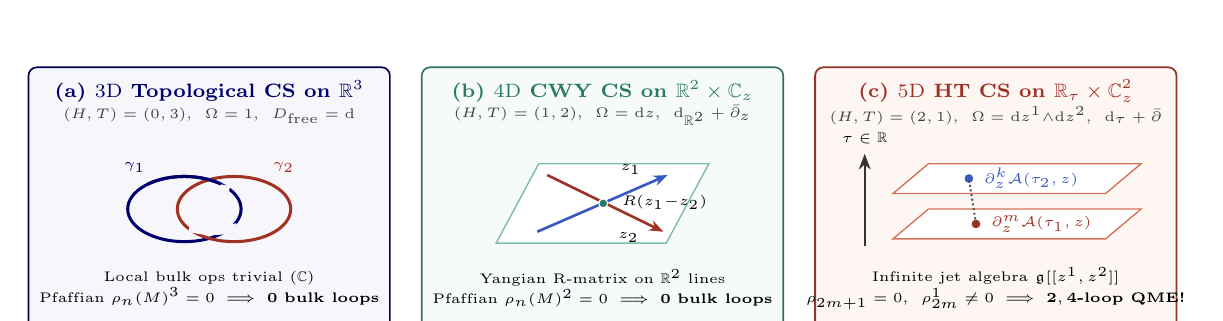
\begin{tikzpicture}[scale=0.90]
  % Panel (a): 3D Topological CS
  \begin{scope}[xshift=-5.55cm]
    \draw[rounded corners=3pt, draw=NavyBlue!65!black, fill=NavyBlue!3, line width=0.6pt] (-2.55,-1.82) rectangle (2.55,1.90);
    \node[font=\scriptsize\bfseries, text=NavyBlue!85!black] at (0,1.56) {(a) $3\mathrm{D}$ Topological CS on $\mathbb{R}^3$};
    \node[font=\tiny, text=black!75] at (0,1.22) {$(H,T)=(0,3)$,\ \ $\Omega = 1$,\ \ $D_{\mathrm{free}}=\dd$};
    % Linked Wilson loops
    \draw[line width=1.1pt, draw=NavyBlue!85!black] (-0.35,-0.10) ellipse (0.80cm and 0.46cm);
    \draw[line width=3.2pt, draw=NavyBlue!3] (0.28,0.16) arc (65:115:0.80cm and 0.46cm);
    \draw[line width=1.1pt, draw=BrickRed!85!black] (0.35,-0.10) ellipse (0.80cm and 0.46cm);
    \draw[line width=3.2pt, draw=NavyBlue!3] (-0.28,-0.36) arc (-115:-65:0.80cm and 0.46cm);
    \draw[line width=1.1pt, draw=NavyBlue!85!black] (-0.35,-0.10) ++(50:0.80cm and 0.46cm) arc (50:130:0.80cm and 0.46cm);
    \node[font=\tiny, text=NavyBlue!85!black] at (-1.05,0.48) {$\gamma_1$};
    \node[font=\tiny, text=BrickRed!85!black] at (1.05,0.48) {$\gamma_2$};
    \node[font=\tiny, align=center] at (0,-1.22) {Local bulk ops trivial ($\mathbb{C}$)\\Pfaffian $\rho_n(M)^3 = 0 \implies \mathbf{0}$ \textbf{bulk loops}};
  \end{scope}

  % Panel (b): 4D CWY CS
  \begin{scope}[xshift=0cm]
    \draw[rounded corners=3pt, draw=PineGreen!65!black, fill=PineGreen!3, line width=0.6pt] (-2.55,-1.82) rectangle (2.55,1.90);
    \node[font=\scriptsize\bfseries, text=PineGreen!80!black] at (0,1.56) {(b) $4\mathrm{D}$ CWY CS on $\mathbb{R}^2\times\mathbb{C}_z$};
    \node[font=\tiny, text=black!75] at (0,1.22) {$(H,T)=(1,2)$,\ \ $\Omega = \dd z$,\ \ $\dd_{\mathbb{R}^2}+\dbar_z$};
    % Crossing spectral lines in R^2 at z_1, z_2
    \draw[fill=white, draw=PineGreen!50, line width=0.5pt] (-1.50,-0.58) -- (-0.90,0.54) -- (1.50,0.54) -- (0.90,-0.58) -- cycle;
    \draw[line width=0.95pt, draw=RoyalBlue!85!black, -{Stealth[length=1.8mm]}] (-0.92,-0.42) -- (0.92,0.38) node[pos=0.86, above left=-1pt, font=\tiny] {$z_1$};
    \draw[line width=0.95pt, draw=BrickRed!85!black, -{Stealth[length=1.8mm]}] (-0.78,0.38) -- (0.86,-0.42) node[pos=0.86, below left=-1pt, font=\tiny] {$z_2$};
    \filldraw[fill=PineGreen!85!black, draw=white] (0.01,-0.02) circle (1.8pt);
    \node[font=\tiny, right=2pt] at (0.06,-0.01) {$R(z_1{-}z_2)$};
    \node[font=\tiny, align=center] at (0,-1.22) {Yangian R-matrix on $\mathbb{R}^2$ lines\\Pfaffian $\rho_n(M)^2 = 0 \implies \mathbf{0}$ \textbf{bulk loops}};
  \end{scope}

  % Panel (c): 5D HT CS
  \begin{scope}[xshift=5.55cm]
    \draw[rounded corners=3pt, draw=BrickRed!75!black, fill=BrickRed!3, line width=0.65pt] (-2.55,-1.82) rectangle (2.55,1.90);
    \node[font=\scriptsize\bfseries, text=BrickRed!85!black] at (0,1.56) {(c) $5\mathrm{D}$ HT CS on $\mathbb{R}_\tau\times\mathbb{C}^2_z$};
    \node[font=\tiny, text=black!75] at (0,1.22) {$(H,T)=(2,1)$,\ \ $\Omega = \dd z^1{\wedge}\dd z^2$,\ \ $\dd_\tau+\dbar$};
    % Vertical tau axis with two C^2 sheets
    \draw[-{Stealth[length=2mm]}, line width=0.75pt, draw=black!80] (-1.85,-0.62) -- (-1.85,0.68) node[above, font=\tiny] {$\tau\in\mathbb{R}$};
    \draw[fill=white, draw=BrickRed!55, line width=0.5pt] (-1.45,-0.52) -- (-0.95,-0.10) -- (2.05,-0.10) -- (1.55,-0.52) -- cycle;
    \draw[fill=white, draw=BrickRed!55, line width=0.5pt] (-1.45,0.12) -- (-0.95,0.54) -- (2.05,0.54) -- (1.55,0.12) -- cycle;
    \filldraw[BrickRed!85!black] (-0.28,-0.31) circle (1.5pt) node[right=2pt, font=\tiny] {$\partial_z^m\mathcal{A}(\tau_1,z)$};
    \filldraw[RoyalBlue!85!black] (-0.38,0.33) circle (1.5pt) node[right=2pt, font=\tiny] {$\partial_z^k\mathcal{A}(\tau_2,z)$};
    \draw[densely dotted, line width=0.7pt, draw=black!70] (-0.28,-0.31) -- (-0.38,0.33);
    \node[font=\tiny, align=center] at (0,-1.22) {Infinite jet algebra $\fg[[z^1,z^2]]$\\$\rho_{2m+1}=0$,\ \ $\rho_{2m}^1\neq 0 \implies \mathbf{2,4}$\textbf{-loop QME!}};
  \end{scope}
\end{tikzpicture}
\caption{The three-step AKSZ Chern--Simons ladder ($T+H=3$). Decreasing real topological directions from $T=3$ and $T=2$ (where $\rho_n(M)^T = 0$ eliminates every bulk loop via \zkcard{topological-t2-pfaffian-vanishing}) to the critical single-time threshold $T=1$ on $\mathbb{R}_\tau\times\mathbb{C}^2_z$ unlocks genuine even-loop bulk quantum anomalies.}
\label{fig:tqft-ladder}
\end{figure}

\begin{table}[H]
\centering
\scriptsize
\setlength{\tabcolsep}{3.6pt}
\renewcommand{\arraystretch}{1.22}
\begin{tabularx}{\textwidth}{@{}>{\raggedright\arraybackslash}p{2.5cm}>{\raggedright\arraybackslash}p{2.4cm}>{\raggedright\arraybackslash}p{2.4cm}>{\raggedright\arraybackslash}X>{\raggedright\arraybackslash}X@{}}
\toprule
\textbf{Five-Dimensional Action} & \textbf{Spacetime Structure} & \textbf{Required Lie Tensor} & \textbf{Classical Form Expression} & \textbf{Relation in This Paper} \\
\midrule
\textbf{HT $5\mathrm{D}$ CS} $S_{\mathrm{cl}}$ \eqref{eq:summary-Scl} & Foliation $\mathbb{R}_\tau\times\mathbb{C}^2_z$ ($\Omega = \dd z^1\wedge\dd z^2$) & Quadratic $\kappa_{AB}$ + Lie $f_{ABC}$ (\emph{any} simple $\fg$) & $\int\dd z^1{\wedge}\dd z^2{\wedge}\big(\frac{1}{2}\kappa(\mathcal{A},D_{\mathrm{free}}\mathcal{A}) + \frac{1}{6}\kappa(\mathcal{A},[\mathcal{A},\mathcal{A}])\big)$ & Classical $O(\hbar^0)$ theory; suffers $2$-loop $[o_2]\neq 0$ for simple $\fg\neq\fsl_2$. \\
\textbf{Topological $5\mathrm{D}$ CS} $\int\mathrm{CS}_5$ & Smooth $M_5$ (fully metric-free) & Symmetric cubic $d_{ABC}$ ($\fsl_{N\ge 3}$ among simple $\fg$) & $\int_{M_5} d_{ABC}\big(A^A\dd A^B\dd A^C + \dots\big)$ ($5$-form transgression of $\tr F^3$) & Restricts on $\Omega^\bullet(\mathbb{R})\widehat{\otimes}\Omega^{0,\bullet}(\mathbb{C}^2)$ to $-3F_D$, giving the $O(\hbar)$ cure $J_1 = a F_D$! \\
\textbf{Mixed Abelian--Simple $\mathrm{CS}_5$} & Smooth $M_5$, gauge $\fg\oplus\mathbb{C}\mathbf{1}$ & $\kappa_{AB}$ on $\fg$ + central $A_{\mathbf{1}}$ ($\fso_5\oplus\mathbb{C}$, $G_2..E_8$) & $\int_{M_5}\big(\chi A_{\mathbf{1}}\wedge\kappa_{AB}F^A_{\fg}{\wedge}F^B_{\fg} + \frac{\gamma}{3}A_{\mathbf{1}}{\wedge}F_{\mathbf{1}}^2\big)$ & Restricts to $j = [p^{(0)}p^{(1)}]T$ in Section~\ref{sec:central-moyal}, curing $[o_2]$ at $\gamma = \ell\chi$! \\
\bottomrule
\end{tabularx}
\caption{Distinction and exact physical dictionary between holomorphic--topological $5\mathrm{D}$ Chern--Simons (built from $\dd z^1\wedge\dd z^2\wedge\mathrm{CS}_3$) and untwisted topological $5\mathrm{D}$ Chern--Simons $5$-forms (whose HT restrictions supply the order-$\hbar$ counterterms in Sections~\ref{sec:classification-o3} and~\ref{sec:central-moyal}).}
\label{tab:cs-ladder}
\end{table}

\begin{proposition}[Restriction of untwisted $5\mathrm{D}$ topological Chern--Simons to $\mathbb{R}\times\mathbb{C}^2$]
\label{prop:cs5-restriction}
Let $\fg = \fsl_N$ ($N \ge 3$) with defining trace $\tr$ and symmetric cubic tensor $d_{ABC} := \tr(T_A\{T_B,T_C\})$ ($d(X,Y,Z) = \tr(X\{Y,Z\})$). On $\mathbb{R}\times\mathbb{C}^2$, let $\mathrm{CS}_5(\mathcal{A}) := \Tr\!\big(\mathcal{A}(\dd_{\mathrm{tot}}\mathcal{A})^2 + \frac{3}{2}\mathcal{A}^3\dd_{\mathrm{tot}}\mathcal{A} + \frac{3}{5}\mathcal{A}^5\big)$ be the standard topological Chern--Simons $5$-form with $\dd_{\mathrm{tot}} = \dd z^i\partial_i + D_{\mathrm{free}}$. Restricting $\mathcal{A}$ to the HT field space $\Omega^\bullet(\mathbb{R})\widehat{\otimes}\Omega^{0,\bullet}(\mathbb{C}^2)\otimes\fsl_N[1]$ (which contains zero $\dd z^1$ or $\dd z^2$ factors) yields modulo total derivatives
\begin{equation}
\label{eq:cs5-to-FD}
\int_{\mathbb{R}\times\mathbb{C}^2}\mathrm{CS}_5(\mathcal{A})\Big|_{\Omega^\bullet(\mathbb{R})\widehat{\otimes}\Omega^{0,\bullet}(\mathbb{C}^2)}
= -\int_{\mathbb{R}\times\mathbb{C}^2}\Omega\wedge d_{ABC}\,\partial_1\mathcal{A}^A\,\partial_2\mathcal{A}^B\,\mathcal{A}^C
= -3\,F_D(\mathcal{A}).
\end{equation}
\end{proposition}

\begin{proof}
A $5$-form on $\mathbb{R}_\tau\times\mathbb{C}^2_z$ has nonzero integral precisely when it saturates both holomorphic differentials $\Omega = \dd z^1\wedge\dd z^2$ alongside $\dd\tau\wedge\dd\bar{z}^{\bar{1}}\wedge\dd\bar{z}^{\bar{2}}$. Because $\mathcal{A} \in \Omega^\bullet(\mathbb{R})\widehat{\otimes}\Omega^{0,\bullet}(\mathbb{C}^2)\otimes\fsl_N[1]$ carries zero $\dd z^i$ factors, every factor of $\dd z^i$ must come from $\dd_{\mathrm{tot}}\mathcal{A} = \dd z^i\partial_i\mathcal{A} + D_{\mathrm{free}}\mathcal{A}$. Both $\frac{3}{2}\mathcal{A}^3\dd_{\mathrm{tot}}\mathcal{A}$ and $\frac{3}{5}\mathcal{A}^5$ contain at most one $\dd_{\mathrm{tot}}$ and therefore vanish identically against $\mathbb{R}\times\mathbb{C}^2$! In the remaining cubic term $\Tr\big(\mathcal{A}(\dd z^1\partial_1\mathcal{A} + \dd z^2\partial_2\mathcal{A})^2\big)$, oddness of $\mathcal{A}$ ($\partial_i\mathcal{A}$ odd, $\dd z^i\partial_i\mathcal{A}$ even) commutes the two factors:
\begin{align*}
\Tr\!\big(\mathcal{A}(\dd z^i\partial_i\mathcal{A})^2\big)
&= \Tr\!\big(\mathcal{A}(\dd z^1\partial_1\mathcal{A}\wedge\dd z^2\partial_2\mathcal{A} + \dd z^2\partial_2\mathcal{A}\wedge\dd z^1\partial_1\mathcal{A})\big) \\
&= -\dd z^1\wedge\dd z^2\wedge\Tr\!\big(\mathcal{A}(\partial_1\mathcal{A}\,\partial_2\mathcal{A} - \partial_2\mathcal{A}\,\partial_1\mathcal{A})\big),
\end{align*}
where moving $\dd z^2$ past the odd form $\partial_1\mathcal{A}$ supplies $-1$ in the first term and moving $\dd z^1$ past $\partial_2\mathcal{A}$ plus $\dd z^2\wedge\dd z^1 = -\Omega$ supplies $+1$ in the second, while $\partial_1\mathcal{A}\,\partial_2\mathcal{A} - \partial_2\mathcal{A}\,\partial_1\mathcal{A} = \{\partial_1\mathcal{A}, \partial_2\mathcal{A}\}_{\mathrm{mat}}$ is the matrix anticommutator because $\partial_1\mathcal{A}, \partial_2\mathcal{A}$ are Grassmann-odd! Thus $\Tr\big(\mathcal{A}\{\partial_1\mathcal{A},\partial_2\mathcal{A}\}_{\mathrm{mat}}\big) = d_{ABC}\partial_1\mathcal{A}^A\partial_2\mathcal{A}^B\mathcal{A}^C = 3\cdot\frac{1}{3!}D(\mathcal{A},\mathcal{A},\mathcal{A})$, proving~\eqref{eq:cs5-to-FD}.
\end{proof}

\subsection{Heat-kernel gauge, Feynman diagram dictionary, and full-wedge contact closure}
\label{subsec:heat-feynman-rules}

Equip $\mathbb{R}_\tau \times \mathbb{C}^2_z$ with the flat Euclidean metric $\dd s^2 = \dd\tau^2 + \delta_{i\bar{\jmath}}\,\dd z^i\,\dd\bar{z}^{\bar{\jmath}}$. Following~\cite{WW} and~\cite[\S2.3]{RepoAllOrders} (\zkcard{costello-heat-kernel-parametrix}), the gauge-fixing operator adjoint to $D_{\mathrm{free}} = \dd\tau\,\partial_\tau + \dd\bar{z}^{\bar{\imath}}\dbar_{\bar{\imath}}$ is
\begin{equation}
\label{eq:Dstar-heat}
D^* := -\iota_{\partial_\tau}\partial_\tau - 4\delta^{\bar{\jmath}i}\iota_{\partial_{\bar{z}^{\bar{\jmath}}}}\partial_i, \qquad
[K_t]_\Omega := \frac{\exp\!\big({-}(\tau^2 + \delta_{i\bar{\jmath}}z^i\bar{z}^{\bar{\jmath}})/(4t)\big)}{4(4\pi t)^{5/2}}\,\dd\tau\wedge\dd\bar{z}^{\bar{1}}\wedge\dd\bar{z}^{\bar{2}},
\end{equation}
normalized so that $\int_{\mathbb{R}\times\mathbb{C}^2}\Omega\wedge[K_t]_\Omega = 1$, with cut-off propagator $P_\varepsilon^L := \int_\varepsilon^L (D^*[K_t]_\Omega)\,\dd t \otimes \kappa^{-1}$. Integrating out relative vertex positions on an $n$-loop connected graph $\Gamma = (V, E)$ converts each internal edge $e \in E$ into a resistor of resistance $t_e > 0$ carrying holomorphic Kirchhoff current $y^e{}_i(t,\lambda)$ ($B^u{}_e y^e{}_i = \lambda^u{}_i$, $C_r{}^e R_{ef} y^f{}_i = 0$, period matrix $M_{rs}(t) = C_r{}^e t_e\delta_{ef} C_s{}^f$, Symanzik polynomial $U_\Gamma = \det M$) and common scalar prefactor $(-1/(8\pi^{5/2}))^n$ ($= -1/(64\pi^5)$ at $n=2$ and $+1/(4096\pi^{10})$ at $n=4$). Figure~\ref{fig:feynman-rules-resistor} displays the complete set of propagator and vertex Feynman rules used throughout Sections~\ref{sec:twoloop}--\ref{sec:central-moyal} together with the electrical-network resistor correspondence and one-loop $C_4$ vanishing.

\begin{figure}[H]
\centering
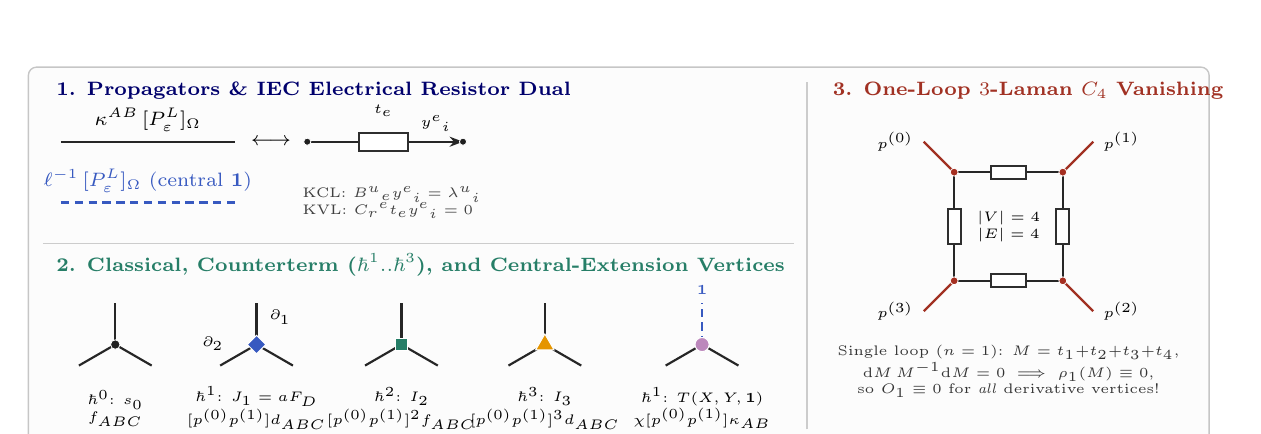
\begin{tikzpicture}[scale=0.92]
  \draw[rounded corners=3pt, draw=gray!45, fill=gray!2, line width=0.5pt] (-8.15,-2.65) rectangle (8.15,2.55);

  % Top-left: Propagators -> IEC resistor
  \node[font=\scriptsize\bfseries, anchor=west, text=NavyBlue!85!black] at (-7.90,2.22) {1. Propagators \& IEC Electrical Resistor Dual};
  \draw[prop] (-7.70,1.52) -- node[above, font=\scriptsize] {$\kappa^{AB}\,[P_\varepsilon^L]_\Omega$} (-5.30,1.52);
  \node[font=\scriptsize] at (-4.80,1.52) {$\longleftrightarrow$};
  \draw[prop] (-4.30,1.52) -- (-3.60,1.52);
  \node[iecres] (R1) at (-3.25,1.52) {};
  \node[above=2pt, font=\tiny] at (R1.north) {$t_e$};
  \draw[prop, -{Stealth[length=1.7mm]}] (-2.90,1.52) -- (-2.15,1.52) node[midway, above, font=\tiny] {$y^e{}_i$};
  \filldraw[v0] (-4.30,1.52) circle (1.4pt);
  \filldraw[v0] (-2.15,1.52) circle (1.4pt);

  \draw[cprop] (-7.70,0.68) -- node[above, font=\scriptsize, text=RoyalBlue!85!black] {$\ell^{-1}\,[P_\varepsilon^L]_\Omega$ (central $\mathbf{1}$)} (-5.30,0.68);
  \node[font=\tiny, align=left, anchor=west, text=black!75] at (-4.50,0.68) {KCL: $B^u{}_e y^e{}_i = \lambda^u{}_i$\\KVL: $C_r{}^e t_e y^e{}_i = 0$};

  % Top-right: 1-loop C_4 vanishing
  \draw[gray!40, line width=0.45pt] (2.60,-2.45) -- (2.60,2.35);
  \node[font=\scriptsize\bfseries, anchor=west, text=BrickRed!85!black] at (2.82,2.22) {3. One-Loop $3$-Laman $C_4$ Vanishing};
  \begin{scope}[xshift=5.38cm, yshift=0.35cm]
    \coordinate (c1) at (-0.75, 0.75);
    \coordinate (c2) at ( 0.75, 0.75);
    \coordinate (c3) at ( 0.75,-0.75);
    \coordinate (c4) at (-0.75,-0.75);
    \draw[prop] (c1) -- node[iecres, scale=0.72] {} (c2);
    \draw[prop] (c2) -- node[iecres, scale=0.72, rotate=90] {} (c3);
    \draw[prop] (c3) -- node[iecres, scale=0.72] {} (c4);
    \draw[prop] (c4) -- node[iecres, scale=0.72, rotate=90] {} (c1);
    \draw[extleg] (c1) -- ++(-0.42, 0.42) node[left, font=\tiny] {$p^{(0)}$};
    \draw[extleg] (c2) -- ++( 0.42, 0.42) node[right, font=\tiny] {$p^{(1)}$};
    \draw[extleg] (c3) -- ++( 0.42,-0.42) node[right, font=\tiny] {$p^{(2)}$};
    \draw[extleg] (c4) -- ++(-0.42,-0.42) node[left, font=\tiny] {$p^{(3)}$};
    \foreach \pt in {c1,c2,c3,c4} \filldraw[vbiv] (\pt) circle (1.55pt);
    \node[font=\tiny, align=center] at (0,0) {$|V|=4$\\$|E|=4$};
  \end{scope}
  \node[font=\tiny, align=center, text=black!80] at (5.38,-1.65) {Single loop ($n=1$): $M = t_1{+}t_2{+}t_3{+}t_4$,\\$\dd M\,M^{-1}\dd M = 0 \implies \rho_1(M) \equiv 0$,\\so $O_1 \equiv 0$ for \emph{all} derivative vertices!};

  % Bottom-left & center: Interaction & Counterterm Vertices
  \draw[gray!40, line width=0.45pt] (-7.95,0.12) -- (2.42,0.12);
  \node[font=\scriptsize\bfseries, anchor=west, text=PineGreen!85!black] at (-7.90,-0.18) {2. Classical, Counterterm ($\hbar^1..\hbar^3$), and Central-Extension Vertices};

  % s_0 vertex
  \begin{scope}[xshift=-6.95cm, yshift=-1.28cm]
    \draw[prop] (0,0) -- (90:0.58);
    \draw[prop] (0,0) -- (210:0.58);
    \draw[prop] (0,0) -- (330:0.58);
    \filldraw[v0] (0,0) circle (1.85pt);
    \node[font=\tiny, align=center] at (0,-0.88) {$\hbar^0$: $s_0$\\$f_{ABC}$};
  \end{scope}

  % J_1 = a F_D vertex
  \begin{scope}[xshift=-5.00cm, yshift=-1.28cm]
    \draw[prop] (0,0) -- (90:0.58) node[pos=0.65, right=1pt, font=\tiny] {$\partial_1$};
    \draw[prop] (0,0) -- (210:0.58) node[pos=0.68, above left=-1pt, font=\tiny] {$\partial_2$};
    \draw[prop] (0,0) -- (330:0.58);
    \node[vj1] at (0,0) {};
    \node[font=\tiny, align=center] at (0,-0.88) {$\hbar^1$: $J_1 = a F_D$\\$[p^{(0)}p^{(1)}]d_{ABC}$};
  \end{scope}

  % I_2 vertex
  \begin{scope}[xshift=-3.00cm, yshift=-1.28cm]
    \draw[prop] (0,0) -- (90:0.58);
    \draw[prop] (0,0) -- (210:0.58);
    \draw[prop] (0,0) -- (330:0.58);
    \node[vi2] at (0,0) {};
    \node[font=\tiny, align=center] at (0,-0.88) {$\hbar^2$: $I_2$\\$[p^{(0)}p^{(1)}]^2 f_{ABC}$};
  \end{scope}

  % I_3 vertex
  \begin{scope}[xshift=-1.02cm, yshift=-1.28cm]
    \draw[prop] (0,0) -- (90:0.58);
    \draw[prop] (0,0) -- (210:0.58);
    \draw[prop] (0,0) -- (330:0.58);
    \node[vi3] at (0,0) {};
    \node[font=\tiny, align=center] at (0,-0.88) {$\hbar^3$: $I_3$\\$[p^{(0)}p^{(1)}]^3 d_{ABC}$};
  \end{scope}

  % Central T vertex
  \begin{scope}[xshift=1.15cm, yshift=-1.28cm]
    \draw[cprop] (0,0) -- (90:0.58) node[above=-1pt, font=\tiny, text=RoyalBlue!85!black] {$\mathbf{1}$};
    \draw[prop] (0,0) -- (210:0.58);
    \draw[prop] (0,0) -- (330:0.58);
    \node[vtcent] at (0,0) {};
    \node[font=\tiny, align=center] at (0,-0.88) {$\hbar^1$: $T(X,Y,\mathbf{1})$\\$\chi[p^{(0)}p^{(1)}]\kappa_{AB}$};
  \end{scope}
\end{tikzpicture}
\caption{Feynman rules of five-dimensional Chern--Simons theory on $\mathbb{R}\times\mathbb{C}^2$, IEC white-rectangle resistor representation of Schwinger edges $t_e$, counterterm vertex markers through $\hbar^3$ (plus the central-extension vertex of Section~\ref{sec:central-moyal}), and exact vanishing of the $1$-loop $3$-Laman box $C_4$.}
\label{fig:feynman-rules-resistor}
\end{figure}

To guarantee at the cochain level (not merely on cohomology classes) that loop obstructions land strictly inside $\Vht$ without acquiring antiholomorphic derivatives or contracted form indices, we establish the finite-cutoff contact lemma of~\cite[Lemma~5.1]{RepoAllOrders}.

\begin{lemma}[Closure of full-wedge holomorphic vertices under total-collapse contacts]
\label{lem:full-wedge-contacts}
For the flat heat kernel~\eqref{eq:Dstar-heat} on $\mathbb{R}\times\mathbb{C}^2$, every total-collapse local contact constructed from cubic vertices in $\Vht$ (carrying arbitrarily many finite holomorphic derivatives) belongs to $\Vht$ and has quartic external arity $4$. Every contact of odd geometric loop number $n = 2m + 1$ vanishes identically. Under simultaneous coordinate rescaling and $\mathrm{U}(1)^2 \subset \mathrm{U}(2)$ rotation $\phi_{r,u}(\tau,z^1,z^2) := (r\tau, r u_1 z^1, r u_2 z^2)$ ($r > 0$, $|u_1|=|u_2|=1$), finite-cutoff propagators satisfy
\begin{equation}
\label{eq:regulated-characters}
\phi_{r,u}^*[K_{r^2 t}]_\Omega = r^{-2}(u_1 u_2)^{-1}[K_t]_\Omega, \qquad
\phi_{r,u}^* P_{r^2\varepsilon}^{r^2 L} = r^{-2}(u_1 u_2)^{-1} P_\varepsilon^L,
\end{equation}
passing by continuity of compactified graph distributions~\cite[Propositions~3.18, 3.21--3.23]{WW} to the limiting local contact.
\end{lemma}

\begin{proof}
Integration by parts expresses holomorphic vertex derivatives as finite sums of holomorphic derivatives on incident kernels and external test forms, which define continuous compactified distributions~\cite{WW} supported at total collapse on the diagonal with purely holomorphic test derivatives. Let $|V|$ and $|E|$ count vertices and internal edges of a connected collapsing cubic graph of loop number $n = |E|-|V|+1$. Tight form saturation in the $3$ real/antiholomorphic directions requires
\begin{equation}
\label{eq:tight-5d-count}
2|E| = 3|V| - 4 \iff |E| = 3n + 1, \qquad |V| = 2n + 2, \qquad E_{\mathrm{ext}} = 3|V| - 2|E| = 4.
\end{equation}
Each extended edge kernel $\Theta_e = [K_{t_e}]_\Omega - \dd t_e\wedge[D^* K_{t_e}]_\Omega$ has total $(\mathbb{R}_{>0}\times X)$-degree $3$. Extracting the $|E|-1$ projective Schwinger differentials leaves spatial $(\tau,\bar{z})$-form degree $3|E| - (|E|-1) = 2|E| + 1 = 3(|V|-1)$, which consists entirely of relative coordinate differences and therefore saturates all $3(|V|-1)$ relative $(\tau,\bar{z}^{\bar{1}},\bar{z}^{\bar{2}})$-differentials! The surviving external factor is purely the diagonal pullback of the full exterior product of the $4$ external superfield jets, placing the contact inside $\Vht$ (self-loops vanish because relative coordinate differences pull back to $0$ on the diagonal). Reflecting relative real coordinates $\Delta\tau \mapsto -\Delta\tau$ multiplies the relative measure and $D^*$ contractions by $(-1)^n$ while leaving holomorphic test jets invariant, killing every odd-$n$ contact. Direct substitution in~\eqref{eq:Dstar-heat} verifies~\eqref{eq:regulated-characters}.
\end{proof}

% ============================================================================
\section{Local Cohomology and Momentum-Conserving Taylor Cochains}
\label{sec:local-cohomology}
% ============================================================================

To turn Feynman graph integrals into exact algebraic equations, we record the Taylor-cochain isomorphism $\Cg \xrightarrow{\simeq} \Vht$ alongside its relation to unrestricted translation-invariant local functionals.

\begin{definition}[Momentum-conserving Taylor cochains $\Cg$ and cochain antibracket]
\label{def:taylor-cochains}
An $r$-cochain $w \in C^{0,r}_{\fg}$ is an alternating multilinear functional of plane-wave inputs $x_q = X_q\ee^{p^{(q)}_i z^i}$ ($q = 0,\dots,r-1$), polynomial in the holomorphic covectors $p^{(q)} \in \mathcal{V}^*$ restricted to the momentum-conservation hyperplane $\sum_{\substack{q=0\\\mathrm{legs}}}^{r-1} p^{(q)}_i = 0$ (the exact Fourier image of quotienting by $D_{z^1}, D_{z^2}$). Full alternation without factorial division is $\Alt w(x_0,\dots,x_{r-1}) := \sum_{\substack{\sigma\in S_r\\\mathrm{perms}}}\sgn(\sigma)\,w(x_{\sigma(0)},\dots,x_{\sigma(r-1)})$. The Chevalley--Eilenberg differential $d_{\mathrm{CE}} : C^{0,r}_{\fg} \to C^{0,r+1}_{\fg}$ and cochain bracket $\{a,b\} \in C^{0,m+n-2}_{\fg}$ ($a \in C^{0,m}_{\fg}$, $b \in C^{0,n}_{\fg}$) are
\begin{align}
\label{eq:ce-and-bracket}
(d_{\mathrm{CE}}w)(x_0,\dots,x_r) &:= \sum_{\substack{0\le q<l\le r\\\mathrm{input\ pairs}}} (-1)^{q+l} w\!\big([X_q,X_l]\ee^{(p^{(q)}+p^{(l)})\cdot z}, x_0, \dots, \widehat{x_q}, \dots, \widehat{x_l}, \dots, x_r\big), \\
\{a, b\}(x_1,\dots,x_{m+n-2}) &:= \frac{1}{(m{-}1)!(n{-}1)!}\Alt\!\Big(a(x_1,\dots,x_{m-1}, T_A\ee^{P\cdot z})\,\kappa^{AB}\,b(T_B\ee^{-P\cdot z}, x_m,\dots,x_{m+n-2})\Big), \nonumber
\end{align}
where $P_i := -\sum_{\substack{q=1\\\mathrm{left\ legs}}}^{m-1} p^{(q)}_i$. For $s_0(X_0,X_1,X_2) := \kappa(X_0,[X_1,X_2])$, $\{s_0, w\} = -d_{\mathrm{CE}}w$. Under $F_w := \frac{1}{r!}\int\Omega\wedge w(\mathcal{A},\dots,\mathcal{A})$, polarization identifies $C^{0,r}_{\fg} \xrightarrow{\simeq} \Vht^{\,r-3}$, so ghost-number-$0$ interactions $I_w \in \Vht^0$ are cubic ($r=3$) and ghost-number-$1$ obstructions $O_w \in \Vht^1$ are quartic ($r=4$).
\end{definition}

\begin{theorem}[Eight-summand Koszul decomposition vs.\ $\eta$-invariant collapse]
\label{thm:local-cohomology}
Let $U_{\mathrm{top}} := \{\tau, \bar{1}, \bar{2}\}$, let $V := M / \sum_{\substack{u\in\{\tau,1,2,\bar{1},\bar{2}\}\\\mathrm{spacetime\ dirs}}} D_u M$ be the full complex of translation-invariant local functionals modulo total derivatives, and let $\Veta := \{F \in V : \iota_{\partial/\partial x^v}F = 0\ \forall\,v \in U_{\mathrm{top}}\}$ (\zkcard{fived-cs-koszul-eta-subcomplex}):
\begin{enumerate}[label=(\alph*),leftmargin=*]
  \item \textbf{Unrestricted eight summands:} $H^g(V) \cong \bigoplus_{\substack{S\subseteq U_{\mathrm{top}}\\\mathrm{form\ subsets}}} \psi_S H^{g+|S|}(\Cg) \cong H^{g+3}(\Cg) \oplus H^{g+2}(\Cg)^{\oplus 3} \oplus H^{g+1}(\Cg)^{\oplus 3} \oplus H^g(\Cg)$. Whenever $\kappa \neq 0$, $V \setminus \Veta$ contains closed non-exact $\mathrm{U}(2)$-invariant ghost-$0$ classes outside $\Vht$:
  \begin{equation}
  \label{eq:G-eps-T-lambda}
  G_\epsilon := \int \dd^2z\wedge\Big(\dd\bar{z}^{\bar{1}}\wedge\kappa_{AB}\partial_2\mathcal{A}^A\mathcal{A}^B - \dd\bar{z}^{\bar{2}}\wedge\kappa_{AB}\partial_1\mathcal{A}^A\mathcal{A}^B\Big), \qquad
  T_\lambda := \int \dd\tau\,\dd^2z\,\dd^2\bar{z}\;\lambda_A \mathcal{A}^A_\tau.
  \end{equation}
  \item \textbf{Contraction-invariant collapse:} The inclusion $\Vht \hookrightarrow \Veta$ is a quasi-isomorphism, and for reductive $\fg = \operatorname{Lie}(G)$, $H^g(\Veta) \cong H^{g+3}(\Cg) \cong H^{g+3}((\Cg)^G)$.
\end{enumerate}
\end{theorem}

\begin{proof}\leavevmode\par\vspace{2pt}
\begin{proofpart}{Proof of (a): Unrestricted eight-summand Koszul decomposition}
Splitting polynomial momenta into total momentum and relative coordinates makes each arity free over $\mathbb{C}[D_\tau, D_z, D_{\bar{z}}]$. Contracting acyclic de Rham pairs $\mathbb{C}[[x^v]] \oplus \mathbb{C}[[x^v]]\dd x^v$ ($v \in U_{\mathrm{top}}$) and conjugating the Koszul resolution by $\Theta := -\sum_{\substack{v\in U_{\mathrm{top}}\\\mathrm{top/antihol}}} \iota_{\partial/\partial x^v}\partial_{\varepsilon_v}$ splits $H^g(V)$ into the eight subsets $S \subseteq U_{\mathrm{top}}$, with $G_\epsilon$ and $T_\lambda$ representing nontrivial $|S| < 3$ classes.
\end{proofpart}
\begin{proofpart}{Proof of (b): Contraction-invariant collapse to $\Vht$}
Hopf shearing over $\Lambda[\iota_{\partial_\tau},\iota_{\partial_{\bar{1}}},\iota_{\partial_{\bar{2}}}]$ isolates $S = U_{\mathrm{top}}$ on $\Veta$, and complete reducibility over $G$ (\zkcard{whitehead-ce-rigidity}) kills nontrivial $G$-isotypic summands via $L_X = [Q_0, \iota_X] = 0$ on cohomology.\qedhere
\end{proofpart}
\end{proof}

% ============================================================================
\section{The Exact Two-Loop Anomaly: Theta Diagrams, Vogel Detector, and Ribbons}
\label{sec:twoloop}
% ============================================================================

\subsection{The two admissible theta Feynman diagrams $\theta(1,3,3)$ and $\theta(2,2,3)$}
\label{subsec:twoloop-thetas}

At geometric loop order $n = 1$, $O_1 = 0$ by Lemma~\ref{lem:full-wedge-contacts} (Figure~\ref{fig:feynman-rules-resistor}). Consequently, for a deformed action $S = S_{\mathrm{cl}} + \hbar J_1 + \hbar^2 I_2 + \mathcal{O}(\hbar^3)$ with $J_1 = F_j, I_2 = F_{i_2} \in \Vht^0$, the order-$\hbar$ and order-$\hbar^2$ master equations are
\begin{equation}
\label{eq:qme-1-2}
d_{\mathrm{CE}} j = 0, \qquad \epsilon\!\left(-d_{\mathrm{CE}} i_2 + \frac{1}{2}\{j, j\}\right) + o_2 = 0,
\end{equation}
where $o_2 \in C^{0,4}_{\fg}$ is the bare two-loop obstruction cochain with $\hbar^2$ stripped. Setting $n = 2$ in~\eqref{eq:tight-5d-count} gives $|V| = 6$ vertices, $|E| = 7$ internal edges, and $4$ external fields placed at $4$ bivalent vertices. Suppressing the $4$ bivalent vertices leaves the unique loopless $2$-vertex cubic theta core with $3$ parallel paths of edge lengths $(n_1,n_2,n_3)$ summing to $7$ ($1 \le n_P \le 3$ so each path has $\le 2$ external legs and induced subgraphs obey $2|E_S|\le 3|V_S|-4$). Up to permutation, \textbf{solely two Feynman diagrams exist}: $\theta(1,3,3)$ and $\theta(2,2,3)$, each with $|\Aut| = 4$, drawn alongside their universal $3$-branch IEC resistor reduction in Figure~\ref{fig:twoloop-thetas-circuit}.

\begin{figure}[H]
\centering
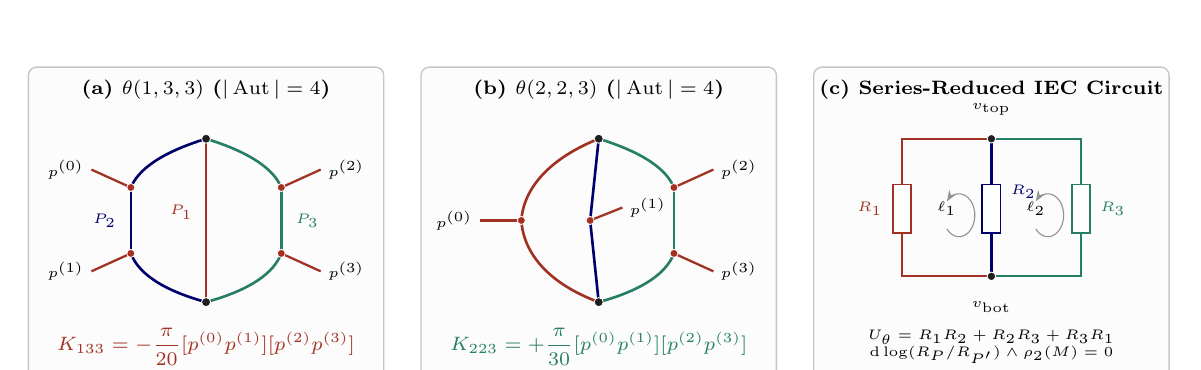
\begin{tikzpicture}[scale=0.91]
  % Panel (a): theta(1,3,3)
  \begin{scope}[xshift=-5.48cm]
    \draw[rounded corners=3pt, draw=gray!45, fill=gray!2, line width=0.5pt] (-2.48,-2.18) rectangle (2.48,2.18);
    \node[font=\scriptsize\bfseries] at (0,1.86) {(a) $\theta(1,3,3)$ ($|\Aut|=4$)};
    \coordinate (top) at (0, 1.18);
    \coordinate (bot) at (0,-1.10);
    % Path 1 (middle length 1, Crimson)
    \draw[line width=0.95pt, draw=BrickRed!85!black] (top) -- node[pos=0.45, left=1pt, font=\tiny, text=BrickRed!85!black] {$P_1$} (bot);
    % Path 2 (left arc length 3, NavyBlue)
    \coordinate (l1) at (-1.05, 0.50);
    \coordinate (l2) at (-1.05,-0.42);
    \draw[line width=0.95pt, draw=NavyBlue!85!black] (top) .. controls (-0.65,0.98) and (-0.95,0.74) .. (l1);
    \draw[line width=0.95pt, draw=NavyBlue!85!black] (l1) -- node[left=1.5pt, font=\tiny, text=NavyBlue!85!black] {$P_2$} (l2);
    \draw[line width=0.95pt, draw=NavyBlue!85!black] (l2) .. controls (-0.95,-0.68) and (-0.65,-0.92) .. (bot);
    % Path 3 (right arc length 3, PineGreen)
    \coordinate (r1) at (1.05, 0.50);
    \coordinate (r2) at (1.05,-0.42);
    \draw[line width=0.95pt, draw=PineGreen!85!black] (top) .. controls (0.65,0.98) and (0.95,0.74) .. (r1);
    \draw[line width=0.95pt, draw=PineGreen!85!black] (r1) -- node[right=1.5pt, font=\tiny, text=PineGreen!85!black] {$P_3$} (r2);
    \draw[line width=0.95pt, draw=PineGreen!85!black] (r2) .. controls (0.95,-0.68) and (0.65,-0.92) .. (bot);
    % External legs
    \draw[extleg] (l1) -- ++(-0.55, 0.25) node[left=-1pt, font=\tiny] {$p^{(0)}$};
    \draw[extleg] (l2) -- ++(-0.55,-0.25) node[left=-1pt, font=\tiny] {$p^{(1)}$};
    \draw[extleg] (r1) -- ++( 0.55, 0.25) node[right=-1pt, font=\tiny] {$p^{(2)}$};
    \draw[extleg] (r2) -- ++( 0.55,-0.25) node[right=-1pt, font=\tiny] {$p^{(3)}$};
    \filldraw[v0] (top) circle (1.8pt);
    \filldraw[v0] (bot) circle (1.8pt);
    \foreach \pt in {l1,l2,r1,r2} \filldraw[vbiv] (\pt) circle (1.6pt);
    \node[font=\scriptsize, text=BrickRed!85!black] at (0,-1.72) {$K_{133} = -\dfrac{\pi}{20}[p^{(0)}p^{(1)}][p^{(2)}p^{(3)}]$};
  \end{scope}

  % Panel (b): theta(2,2,3)
  \begin{scope}[xshift=0cm]
    \draw[rounded corners=3pt, draw=gray!45, fill=gray!2, line width=0.5pt] (-2.48,-2.18) rectangle (2.48,2.18);
    \node[font=\scriptsize\bfseries] at (0,1.86) {(b) $\theta(2,2,3)$ ($|\Aut|=4$)};
    \coordinate (top2) at (0, 1.18);
    \coordinate (bot2) at (0,-1.10);
    \coordinate (m0) at (-0.12, 0.04);
    \coordinate (l0) at (-1.08, 0.04);
    \coordinate (r21) at (1.05, 0.50);
    \coordinate (r22) at (1.05,-0.42);
    % Path 1 (left length 2, Crimson)
    \draw[line width=0.95pt, draw=BrickRed!85!black] (top2) .. controls (-0.7,0.90) and (-1.05,0.48) .. (l0);
    \draw[line width=0.95pt, draw=BrickRed!85!black] (l0) .. controls (-1.05,-0.42) and (-0.7,-0.84) .. (bot2);
    % Path 2 (middle length 2, NavyBlue)
    \draw[line width=0.95pt, draw=NavyBlue!85!black] (top2) -- (m0) -- (bot2);
    % Path 3 (right length 3, PineGreen)
    \draw[line width=0.95pt, draw=PineGreen!85!black] (top2) .. controls (0.65,0.98) and (0.95,0.74) .. (r21);
    \draw[line width=0.95pt, draw=PineGreen!85!black] (r21) -- (r22);
    \draw[line width=0.95pt, draw=PineGreen!85!black] (r22) .. controls (0.95,-0.68) and (0.65,-0.92) .. (bot2);
    % External legs
    \draw[extleg] (l0) -- ++(-0.58, 0.0) node[left=-1pt, font=\tiny] {$p^{(0)}$};
    \draw[extleg] (m0) -- ++(0.45, 0.18) node[right=-1pt, font=\tiny] {$p^{(1)}$};
    \draw[extleg] (r21) -- ++(0.55, 0.25) node[right=-1pt, font=\tiny] {$p^{(2)}$};
    \draw[extleg] (r22) -- ++(0.55,-0.25) node[right=-1pt, font=\tiny] {$p^{(3)}$};
    \filldraw[v0] (top2) circle (1.8pt);
    \filldraw[v0] (bot2) circle (1.8pt);
    \foreach \pt in {l0,m0,r21,r22} \filldraw[vbiv] (\pt) circle (1.6pt);
    \node[font=\scriptsize, text=PineGreen!85!black] at (0,-1.72) {$K_{223} = +\dfrac{\pi}{30}[p^{(0)}p^{(1)}][p^{(2)}p^{(3)}]$};
  \end{scope}

  % Panel (c): Universal 3-Branch IEC Resistor Circuit
  \begin{scope}[xshift=5.48cm]
    \draw[rounded corners=3pt, draw=gray!45, fill=gray!2, line width=0.5pt] (-2.48,-2.18) rectangle (2.48,2.18);
    \node[font=\scriptsize\bfseries] at (0,1.86) {(c) Series-Reduced IEC Circuit};
    \coordinate (nt) at (0, 1.18);
    \coordinate (nb) at (0,-0.74);
    % Left branch R_1
    \draw[line width=0.8pt, draw=BrickRed!85!black] (nt) -| (-1.25,0.52);
    \node[iecres, rotate=90, draw=BrickRed!85!black] at (-1.25,0.20) {};
    \node[left=3.5pt, font=\tiny, text=BrickRed!85!black] at (-1.25,0.20) {$R_1$};
    \draw[line width=0.8pt, draw=BrickRed!85!black] (-1.25,-0.12) |- (nb);
    % Middle branch R_2
    \draw[line width=0.8pt, draw=NavyBlue!85!black] (nt) -- (0,0.52);
    \node[iecres, rotate=90, draw=NavyBlue!85!black] at (0,0.20) {};
    \node[right=3.5pt, font=\tiny, text=NavyBlue!85!black] at (0,0.44) {$R_2$};
    \draw[line width=0.8pt, draw=NavyBlue!85!black] (0,-0.12) -- (nb);
    % Right branch R_3
    \draw[line width=0.8pt, draw=PineGreen!85!black] (nt) -| (1.25,0.52);
    \node[iecres, rotate=90, draw=PineGreen!85!black] at (1.25,0.20) {};
    \node[right=3.5pt, font=\tiny, text=PineGreen!85!black] at (1.25,0.20) {$R_3$};
    \draw[line width=0.8pt, draw=PineGreen!85!black] (1.25,-0.12) |- (nb);
    % Cycle arrows
    \draw[-{Stealth[length=1.4mm]}, thin, gray!85] (-0.62,-0.08) arc (-140:140:0.22cm and 0.30cm);
    \node[font=\tiny] at (-0.62,0.20) {$\ell_1$};
    \draw[-{Stealth[length=1.4mm]}, thin, gray!85] (0.62,-0.08) arc (-140:140:0.22cm and 0.30cm);
    \node[font=\tiny] at (0.62,0.20) {$\ell_2$};
    \filldraw[v0] (nt) circle (1.7pt) node[above=1pt, font=\tiny] {$v_{\mathrm{top}}$};
    \filldraw[v0] (nb) circle (1.7pt) node[below=1.5pt, font=\tiny] {$v_{\mathrm{bot}}$};
    \node[font=\tiny, align=center] at (0,-1.72) {$U_\theta = R_1 R_2 + R_2 R_3 + R_3 R_1$\\$\dd\log(R_P/R_{P'})\wedge\rho_2(M) = 0$};
  \end{scope}
\end{tikzpicture}
\caption{The two surviving bare two-loop Feynman diagrams on $\mathbb{R}\times\mathbb{C}^2$ with color-coded paths $P_1$ (crimson), $P_2$ (blue), $P_3$ (green) and their series-reduced three-branch IEC resistor network.}
\label{fig:twoloop-thetas-circuit}
\end{figure}

\begin{proposition}[Evaluation of $K_{133}, K_{223}$ and bare obstruction assembly]
\label{prop:twoloop-evaluation}
On $\mathbb{R}\times\mathbb{C}^2$, in the calibrated vertex/edge orientation of~\cite[\S2.1]{RepoAllOrders}:
\begin{align}
\label{eq:K133-K223}
K_{133} &= -\frac{1}{2}\frac{\Gamma(\frac{5}{2})\Gamma(\frac{1}{2})^2}{0!\,2!\,2!\,\Gamma(\frac{7}{2})}[p^{(0)}p^{(1)}][p^{(2)}p^{(3)}] = -\frac{\pi}{20}[p^{(0)}p^{(1)}][p^{(2)}p^{(3)}], \nonumber\\
K_{223} &= +\frac{1}{2}\frac{\Gamma(\frac{3}{2})^2\Gamma(\frac{1}{2})}{1!\,1!\,2!\,\Gamma(\frac{7}{2})}[p^{(0)}p^{(1)}][p^{(2)}p^{(3)}] = +\frac{\pi}{30}[p^{(0)}p^{(1)}][p^{(2)}p^{(3)}].
\end{align}
Setting $F_\Gamma := \Alt([p^{(0)}p^{(1)}][p^{(2)}p^{(3)}]W_\Gamma)$ where $W_\Gamma$ contracts the $6$ cubic structure tensors across the $7$ inverse pairings $\kappa^{AB}$, and $\nu = -U/(64\pi^5)$, the bare two-loop cochain is
\begin{equation}
\label{eq:o2-assembled}
o_2 = \frac{\pi\nu}{240}\big({-}3 F_{133} + 2 F_{223}\big) = -\frac{U}{15360\pi^4}\big({-}3 F_{133} + 2 F_{223}\big).
\end{equation}
For $\fg = \fsl_N$ ($\kappa = \tr$) with $\beta := d_{\mathrm{CE}}([p^{(0)}p^{(1)}]^2 f)$, $F_{133} + F_{223} = 2N^2\beta$, giving $o_2 = \pi\nu\big(\frac{1}{48}F_{223} - \frac{N^2}{40}\beta\big)$ and cohomology class $[o_2] = -\frac{U}{3072\pi^4}[F_{223}]$.
\end{proposition}

\begin{proof}
Parameterize path edge resistances as $t_{P,q} = R_P x_{P,q}$ ($x_P \in \Delta^{n_P-1}$). In cycle basis $C_3 = (P_1-P_2, P_2-P_3)$ (Figure~\ref{fig:twoloop-thetas-circuit}c), $M = \begin{psmallmatrix}R_1+R_2 & -R_2\\ -R_2 & R_2+R_3\end{psmallmatrix}$ has $\det M = U_\theta$ and Pfaffian $2$-form $\rho_2(M) = \frac{R_1\dd R_2\wedge\dd R_3 - R_2\dd R_1\wedge\dd R_3 + R_3\dd R_1\wedge\dd R_2}{2U_\theta^{3/2}}$. Because $\dd\log(R_1/R_2)\wedge\rho_2(M) = \dd\log(R_2/R_3)\wedge\rho_2(M) = 0$, wedging $\rho_2(M)$ annihilates every endpoint voltage-division differential $V_i\dd\log(R_P/R_{P'})$ in $\psi_{1,i}\wedge\psi_{2,i}$! Each simplex $\Delta^{n_P-1}$ then integrates trivially to $1/(n_P-1)!$, while parallel conductances $w_P = R_P^{-1}/(R_1^{-1}+R_2^{-1}+R_3^{-1}) \in \Delta^2$ integrate via Dirichlet's beta formula $\int_{\Delta^2}\prod_{P=1}^3 w_P^{7/2-n_P-1}\dd^2w = \prod_{P=1}^3\Gamma(\frac{7}{2}-n_P)/\Gamma(\frac{7}{2})$, giving~\eqref{eq:K133-K223}. Dividing by $|\Aut| = 4$ gives $-\frac{1}{80}$ and $+\frac{1}{120}$, i.e.~\eqref{eq:o2-assembled}. Direct $\fsl_N$ completeness contraction~\eqref{eq:traceless-completeness} produces
\begin{align}
\label{eq:W133-W223-traces}
W_{133} &= 2\tr(0123) + (2{+}N^2)\tr(0132) - 4\tr(0213) + (2{+}N^2)\tr(0231) - 4\tr(0312) + 2\tr(0321) \nonumber\\
&\quad + 6N\tr(01)\tr(23), \nonumber\\
W_{223} &= -2\tr(0123) - 2\tr(0132) + 4\tr(0213) - 2\tr(0231) + 4\tr(0312) - 2\tr(0321) \nonumber\\
&\quad - 4N\tr(01)\tr(23) + 2N\tr(02)\tr(13) + 2N\tr(03)\tr(12),
\end{align}
whose full alternation cancels all double-trace terms in $F_{133} + F_{223} = 2N^2\beta$ and leaves $-\frac{3}{240}(-F_{223}+2N^2\beta)+\frac{2}{240}F_{223} = \frac{1}{48}F_{223} - \frac{N^2}{40}\beta$.
\end{proof}

\subsection{Vogel universal detector and 't~Hooft ribbon worldsheet topology}
\label{subsec:vogel-ribbon}

Notice in~\eqref{eq:W133-W223-traces} that all single-trace pieces of $o_2$ are $d_{\mathrm{CE}}$-exact ($-\frac{N^2}{40}\beta$); under 't~Hooft scaling $\hbar = \lambda_{\mathrm{tH}}/N$ in $\fgl_N$, the non-exact class $[o_2]$ lives purely in \textbf{planar ($h=0$, Euler $6 - 7 + f_{\mathrm{faces}} = 2 - b_{\mathrm{bdry}}$) double-trace cylinder} ($\frac{U\lambda_{\mathrm{tH}}^2}{512\pi^4 N}$) and \textbf{triple-trace pair-of-pants} ($-\frac{U\lambda_{\mathrm{tH}}^2}{256\pi^4 N^2}$) worldsheets (Figure~\ref{fig:ribbon-vogel}a)! To classify $[o_2]$ uniformly across \emph{every} complex simple Lie algebra $\fg$ without choosing matrix representations, adopt Killing normalization $\kappa = \kappa^{\mathrm{Kill}}$. On the $[p^{(0)}p^{(1)}][p^{(0)}p^{(2)}]$ momentum slice of any $G\times\SL_2(\mathbb{C})$-invariant $4$-cochain $X$, define the two full Killing contractions $\ell_{\kappa\kappa}(X)$ against $\kappa(X_0,X_1)\kappa(X_2,X_3)$ and $\ell_{ff}(X)$ against $\kappa([X_0,X_1],[X_2,X_3])$ (Figure~\ref{fig:ribbon-vogel}b).

\begin{figure}[H]
\centering
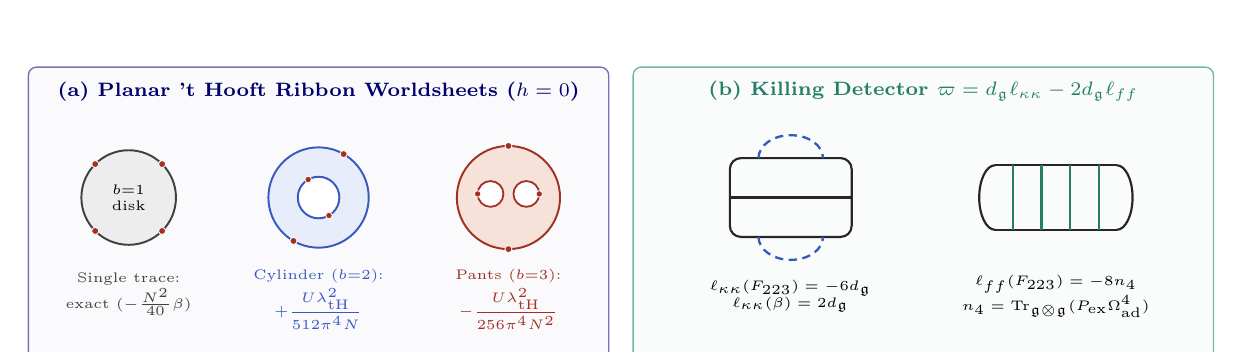
\begin{tikzpicture}[scale=0.91]
  % Panel (a): Ribbon worldsheets
  \begin{scope}[xshift=-4.22cm]
    \draw[rounded corners=3pt, draw=NavyBlue!55, fill=NavyBlue!2, line width=0.5pt] (-4.05,-2.08) rectangle (4.05,2.04);
    \node[font=\scriptsize\bfseries, text=NavyBlue!85!black] at (0,1.70) {(a) Planar 't~Hooft Ribbon Worldsheets ($h=0$)};
    % Disk (exact)
    \begin{scope}[xshift=-2.65cm, yshift=0.22cm]
      \filldraw[fill=gray!14, draw=black!75, line width=0.7pt] (0,0) circle (0.66cm);
      \foreach \ang in {45,135,225,315} \filldraw[vbiv] (\ang:0.66cm) circle (1.4pt);
      \node[font=\tiny, align=center] at (0,0) {$b{=}1$\\disk};
      \node[font=\tiny, align=center, text=black!75] at (0,-1.35) {Single trace:\\exact ($-\frac{N^2}{40}\beta$)};
    \end{scope}
    % Cylinder (double trace)
    \begin{scope}[xshift=0cm, yshift=0.22cm]
      \filldraw[fill=RoyalBlue!12, draw=RoyalBlue!85!black, line width=0.7pt] (0,0) circle (0.70cm);
      \filldraw[fill=white, draw=RoyalBlue!85!black, line width=0.7pt] (0,0) circle (0.29cm);
      \filldraw[vbiv] (60:0.70cm) circle (1.4pt);
      \filldraw[vbiv] (240:0.70cm) circle (1.4pt);
      \filldraw[vbiv] (120:0.29cm) circle (1.3pt);
      \filldraw[vbiv] (300:0.29cm) circle (1.3pt);
      \node[font=\tiny, align=center, text=RoyalBlue!85!black] at (0,-1.42) {Cylinder ($b{=}2$):\\[1pt]$+\dfrac{U\lambda_{\mathrm{tH}}^2}{512\pi^4 N}$};
    \end{scope}
    % Pair of pants (triple trace)
    \begin{scope}[xshift=2.65cm, yshift=0.22cm]
      \filldraw[fill=BrickRed!10, draw=BrickRed!85!black, line width=0.7pt] (0,0) circle (0.72cm);
      \filldraw[fill=white, draw=BrickRed!85!black, line width=0.65pt] (-0.25,0.05) circle (0.18cm);
      \filldraw[fill=white, draw=BrickRed!85!black, line width=0.65pt] ( 0.25,0.05) circle (0.18cm);
      \filldraw[vbiv] (90:0.72cm) circle (1.4pt);
      \filldraw[vbiv] (270:0.72cm) circle (1.4pt);
      \filldraw[vbiv] (-0.43,0.05) circle (1.3pt);
      \filldraw[vbiv] ( 0.43,0.05) circle (1.3pt);
      \node[font=\tiny, align=center, text=BrickRed!85!black] at (0,-1.42) {Pants ($b{=}3$):\\[1pt]$-\dfrac{U\lambda_{\mathrm{tH}}^2}{256\pi^4 N^2}$};
    \end{scope}
  \end{scope}

  % Panel (b): Killing detector contractions
  \begin{scope}[xshift=4.22cm]
    \draw[rounded corners=3pt, draw=PineGreen!55, fill=PineGreen!2, line width=0.5pt] (-4.05,-2.08) rectangle (4.05,2.04);
    \node[font=\scriptsize\bfseries, text=PineGreen!85!black] at (0,1.70) {(b) Killing Detector $\varpi = d_{\fg}\ell_{\kappa\kappa} - 2d_{\fg}\ell_{ff}$};
    % ell_kk
    \begin{scope}[xshift=-1.85cm, yshift=0.22cm]
      \draw[prop, rounded corners=4pt] (-0.85,0.55) rectangle (0.85,-0.55);
      \draw[prop] (-0.85,0) -- (0.85,0);
      \draw[line width=0.85pt, densely dashed, draw=RoyalBlue!85!black] (-0.45,0.55) arc (180:0:0.45cm and 0.32cm);
      \draw[line width=0.85pt, densely dashed, draw=RoyalBlue!85!black] (-0.45,-0.55) arc (-180:0:0.45cm and 0.32cm);
      \node[font=\tiny, align=center] at (0,-1.38) {$\ell_{\kappa\kappa}(F_{223}) = -6d_{\fg}$\\$\ell_{\kappa\kappa}(\beta) = 2d_{\fg}$};
    \end{scope}
    % ell_ff -> 4-rung Casimir
    \begin{scope}[xshift=1.85cm, yshift=0.22cm]
      \draw[prop] (-0.85,0.45) -- (0.85,0.45);
      \draw[prop] (-0.85,-0.45) -- (0.85,-0.45);
      \foreach \xx in {-0.6,-0.2,0.2,0.6} \draw[line width=0.8pt, draw=PineGreen!85!black] (\xx,0.45) -- (\xx,-0.45);
      \draw[prop] (-0.85,0.45) arc (90:270:0.22cm and 0.45cm);
      \draw[prop] (0.85,0.45) arc (90:-90:0.22cm and 0.45cm);
      \node[font=\tiny, align=center] at (0,-1.38) {$\ell_{ff}(F_{223}) = -8n_4$\\$n_4 = \Tr_{\fg\otimes\fg}(P_{\mathrm{ex}}\Omega_{\mathrm{ad}}^4)$};
    \end{scope}
  \end{scope}
\end{tikzpicture}
\caption{(a) Planar ribbon decomposition of $o_2$: single-trace disk diagrams are exact, while cylinder and pair-of-pants worldsheets carry $[F_{223}]$. (b) Closing external legs with $\kappa\otimes\kappa$ versus $f\otimes f$ reduces $[o_2]$ to the fourth split-Casimir trace $n_4$.}
\label{fig:ribbon-vogel}
\end{figure}

\begin{theorem}[Vogel universal detector and nontriviality of the bare two-loop anomaly]
\label{thm:bare-anomaly}
For every complex simple Lie algebra $\fg$ in Killing normalization, the invariant coboundary space in $C^4_{\mathrm{inv}}(2,2)$ is $1$-dimensional, spanned by $\beta = d_{\mathrm{CE}}([p^{(0)}p^{(1)}]^2 f)$, which satisfies $\ell_{\kappa\kappa}(\beta) = 2d_{\fg}$ and $\ell_{ff}(\beta) = d_{\fg}$. Consequently $\varpi := d_{\fg}\ell_{\kappa\kappa} - 2d_{\fg}\ell_{ff}$ annihilates every invariant coboundary ($\varpi(\beta) = 0$) and evaluates on $F_{223} = -F_{133} + \frac{1}{2}\beta$ via Vogel parameters $(v_1,v_2,v_3)$ ($t_V = v_1+v_2+v_3$, \zkcard{vogel-universal-plane}) to
\begin{align}
\label{eq:vogel-n4}
8n_4 - 3d_{\fg} &= -\frac{3d_{\fg}(t_V+v_1)(t_V+v_2)(t_V+v_3)}{2t_V^3} = \frac{3d_{\fg}(d_{\fg}-3)v_1 v_2 v_3}{4t_V^3}, \\
\label{eq:vogel-varpi}
\varpi(o_2) &= \frac{\pi\nu}{24}d_{\fg}(8n_4 - 3d_{\fg}) \neq 0 \quad \Longleftrightarrow \quad [o_2] \neq 0 \quad \Longleftrightarrow \quad \fg \not\cong \fsl_2.
\end{align}
\end{theorem}

\begin{proof}
Since $\dim(\Lambda^3\fg^*)^{\fg} = 1$ (\zkcard{whitehead-ce-rigidity}), the sole $\fg\times\SL_2(\mathbb{C})$-invariant degree-$4$ cubic primitive is $[p^{(0)}p^{(1)}]^2 f$, so $B^4 \cap C^4_{\mathrm{inv}}(2,2) = \mathbb{C}\beta$. Before alternation, the pairings $(01)(23),(02)(13),(03)(12)$ on $W_{223}$ contract with $\kappa\otimes\kappa$ to $(-\frac{1}{2}d_{\fg},\frac{1}{4}d_{\fg},\frac{1}{4}d_{\fg})$ and with $f\otimes f$ to $(0, n_4, n_4)$ ($n_4 = \Tr_{\fg\otimes\fg}(P_{\mathrm{ex}}\Omega_{\mathrm{ad}}^4)$). Full alternation applies weights $(8,-4,-4)$ and $(0,-4,-4)$, yielding $\ell_{\kappa\kappa}(F_{223}) = -6d_{\fg}$, $\ell_{ff}(F_{223}) = -8n_4$, and $\varpi(F_{223}) = 2d_{\fg}(8n_4 - 3d_{\fg}) = -\varpi(F_{133})$. Substituting Mkrtchyan--Sergeev--Veselov's fourth Casimir identity~\cite{MSV} $n_4 = d_{\fg}\big[\frac{3t_V(v_1^2+v_2^2+v_3^2)-(v_1^3+v_2^3+v_3^3)}{16t_V^3} - \frac{1}{8}\big]$ gives~\eqref{eq:vogel-n4}. Table~\ref{tab:vogel-values} evaluates $8n_4 - 3d_{\fg}$ across every simple root family, vanishing solely at $\fsl_2 = \fso_3 = \fsp_2$ (where directly $F_{133} = \frac{7}{2}\beta$ and $F_{223} = -3\beta$; note $\fso_4 \cong \fsl_2\oplus\fsl_2$ is reducible). Rescaling $\kappa \mapsto c\kappa$ ($c \neq 0$) scales $o_2$ by $c^{6-7} = c^{-1}$ and preserves nontriviality.
\end{proof}

\begin{table}[H]
\centering
\scriptsize
\setlength{\tabcolsep}{4.8pt}
\renewcommand{\arraystretch}{1.32}
\begin{tabular}{@{}llll|llll@{}}
\toprule
$\fg$ & $(v_1, v_2, v_3)$ & $t_V$ & $8n_4 - 3d_{\fg}$ & $\fg$ & $(v_1, v_2, v_3)$ & $t_V$ & $8n_4 - 3d_{\fg}$ \\
\midrule
$\fsl_N$ ($N\ge 2$) & $(-2, 2, N)$ & $N$ & $-\dfrac{3(N^2{-}1)(N^2{-}4)}{N^2}$ & $G_2$ & $(-2, \frac{10}{3}, \frac{8}{3})$ & $4$ & $-\dfrac{385}{12}$ \\[4pt]
$\fso_N$ ($N\ge 3$) & $(-2, 4, N{-}4)$ & $N{-}2$ & $-\dfrac{3N(N{-}1)(N{-}3)(N{-}4)(N{+}2)}{2(N{-}2)^3}$ & $F_4$ & $(-2, 5, 6)$ & $9$ & $-\dfrac{12740}{81}$ \\[4pt]
$\fsp_N$ ($2\mid N$) & $(-2, 1, \frac{N+4}{2})$ & $\frac{N+2}{2}$ & $-\dfrac{3N(N{-}2)(N{+}1)(N{+}3)(N{+}4)}{2(N{+}2)^3}$ & $E_6$ & $(-2, 6, 8)$ & $12$ & $-\dfrac{975}{4}$ \\[4pt]
$E_7$ & $(-2, 8, 12)$ & $18$ & $-\dfrac{34580}{81}$ & $E_8$ & $(-2, 12, 20)$ & $30$ & $-\dfrac{12152}{15}$ \\
\bottomrule
\end{tabular}
\caption{Exact Vogel triples and two-loop anomaly detector values $8n_4 - 3d_{\fg}$ across all complex simple Lie algebras ($\fsp_N$ denotes even defining dimension $N$).}
\label{tab:vogel-values}
\end{table}

\begin{example}[Low-rank consistency: $\fsl_2 = \fso_3 = \fsp_2$ vanishing vs.\ $\fso_5 = \fsp_4$ agreement]
\label{ex:vogel-checks}
Evaluating the classical-series formulas in Table~\ref{tab:vogel-values} across accidental low-rank Lie algebra isomorphisms (\zkcard{low-rank-isomorphisms-cubic-invariants}) confirms both boundary cases:
\begin{enumerate}[label=(\alph*),leftmargin=*]
  \item \textbf{Three presentations of $\fsl_2$:} Setting $N=2$ in $-\frac{3(N^2-1)(N^2-4)}{N^2}$ kills $(N^2-4)=0$; setting $N=3$ in $\fso_N$ kills $(N-3)=0$; and setting $N=2$ in $\fsp_N$ kills $(N-2)=0$, yielding $8n_4 - 3d_{\fg} = 0$ identically across $\fsl_2 \cong \fso_3 \cong \fsp_2$.
  \item \textbf{Isomorphism $\fso_5 \cong \fsp_4$:} For $\fso_5$ ($N=5$), $8n_4 - 3d_{\fg} = -\frac{3\cdot 5\cdot 4\cdot 2\cdot 1\cdot 7}{2\cdot 3^3} = -\frac{840}{54} = -\frac{140}{9}$; for $\fsp_4$ ($N=4$, $t_V = 3$), $-\frac{3\cdot 4\cdot 2\cdot 5\cdot 7\cdot 8}{2\cdot 6^3} = -\frac{6720}{432} = -\frac{140}{9}$, matching identically.
\end{enumerate}
\end{example}

% ============================================================================
\section{Semisimple Classification, First Three Counterterms, and Order-3 Diagrams}
\label{sec:classification-o3}
% ============================================================================

\subsection{Rank-uniform polynomial primitive and semisimple classification}
\label{subsec:nogo-semisimple}

In \path{flagship.tex}, the non-type-$A$ no-go theorem relied on computer-verified root tables up to rank~$40$. The updated \texttt{5d-cs-all-orders} manuscript~\cite[\S3]{RepoAllOrders} replaces finite checks by two uniform analytical arguments valid at \emph{every} rank and \emph{every} polynomial derivative bidegree. First, by \zkcard{low-rank-isomorphisms-cubic-invariants}, $\dim(\fg^{*\otimes 3})^{\fg} = \#\{r : \langle\theta,\alpha_r^\vee\rangle \neq 0\}$ equals $2$ for $\fsl_{N\ge 3}$ (spanned by $f$ and $d$) and $1$ (spanned by $f$) for every other simple $\fg$. Second, an explicit radial line-integral primitive kills all positive-degree cocycles in the $f$-channel:

\begin{lemma}[Vanishing of all positive-derivative cocycles in the alternating $f$-channel]
\label{lem:f-channel-primitive}
Let $\fg$ be complex simple with $(\fg^{*\otimes 3})^{\fg} = \mathbb{C}f$. In the momentum-conserving complex $\Cg$, without assuming rotation or dilation equivariance,
\begin{equation}
\label{eq:f-channel-h3}
H^3(\Cg)_{(0,0)} = \mathbb{C}[s_0], \qquad H^3(\Cg)_{(w_1,w_2)} = 0 \quad (\forall\,w_1 + w_2 > 0).
\end{equation}
\end{lemma}

\begin{proof}
Complete reducibility of the adjoint group at fixed momentum degree restricts cohomology to $G$-invariant cochains $P(p,q)\kappa(X,[Y,Z])$ ($p + q + r = 0$), where full alternation enforces $P(p,q) = P(q,p) = P(p, -p-q)$. Because the three four-color contractions $\kappa([X_1,X_2],[X_3,X_4])$, $\kappa([X_1,X_3],[X_2,X_4])$, $\kappa([X_1,X_4],[X_2,X_3])$ obey solely the Jacobi relation (verified on $(X,X,Y,Y)$ and $(X,Y,Y,X)$ inside any root $\fsl_2 \subset \fg$), $d_{\mathrm{CE}}(P\,f) = 0$ holds precisely when
\begin{equation}
\label{eq:cauchy-2cocycle}
P(p, q) + P(p + q, r) = P(q, r) + P(p, q + r) \qquad (\forall\,p, q, r \in \mathcal{V}^*).
\end{equation}
Setting $q = 0$ gives $P(p,0) = P(0,0)$. Differentiating~\eqref{eq:cauchy-2cocycle} in $r$ at $0$ along $u \in \mathcal{V}^*$ yields $D_2 P(p,q)[u] = D_2 P(p+q,0)[u] - D_2 P(q,0)[u]$. Symmetry $P(p,q) = P(q,p)$ implies that the polynomial $1$-form $v \mapsto D_2 P(v,0)$ is closed, with explicit polynomial radial primitive
\begin{equation}
\label{eq:radial-H}
H(v) := \int_0^1 D_2 P(tv, 0)[v]\,\dd t, \qquad P(p, q) = P(0,0) + H(p+q) - H(p) - H(q).
\end{equation}
Using $P(p, -p-q) = P(p,q)$ at $q = -v, p = v$ gives $H(v) + H(-v) = 0$, so the $2$-cochain $-H(p)\kappa(X,Y)$ ($p+q=0$) is alternating and satisfies $d_{\mathrm{CE}}(-H(p)\kappa(X,Y)) = [H(p+q)-H(p)-H(q)]f$, removing every positive-degree term of $P$ while preserving bidegree $(w_1,w_2)$! At $(0,0)$, $\kappa(X,Y)$ is symmetric so zero alternating $2$-cochains exist, leaving $\mathbb{C}[s_0]$.
\end{proof}

\begin{theorem}[Uniform simple no-go theorem]
\label{thm:uniform-nogo}
For every complex simple Lie algebra $\fg \notin \{\fsl_N\}_{N\ge 2}$ with any nondegenerate invariant bilinear form, zero solutions of the QME~\eqref{eq:qme-1-2} exist in $\Vht$ through order $\hbar^2$, even without assuming $G$-invariance or $\mathrm{U}(2)$-equivariance of $J_1$.
\end{theorem}

\begin{proof}
By Lemma~\ref{lem:f-channel-primitive}, any $d_{\mathrm{CE}}$-closed $j \in C^{0,3}_{\fg}$ satisfies $[j] = c_0[s_0]$ in $H^3(\Cg)$. Since $\{s_0, s_0\} = 0$ and the antibracket descends to cohomology, $[\frac{1}{2}\{j, j\}] = 0$, contradicting $\epsilon[\frac{1}{2}\{j,j\}] = -[o_2] \neq 0$ (Theorem~\ref{thm:bare-anomaly}).
\end{proof}

\begin{corollary}[Semisimple direct-sum classification]
\label{cor:semisimple-class}
Let $\fg = \bigoplus_{\substack{u\\\mathrm{ideals}}}\fg_u$ be a complex semisimple Lie algebra with any nondegenerate invariant symmetric bilinear form. Under the local heat-kernel hypotheses of Theorem~\ref{thm:all-orders-traceless}, $\fg$ admits an all-order $\mathrm{U}(2)$-equivariant formal quantization in $\Vht$ precisely when
\begin{equation}
\label{eq:semisimple-iff}
\fg = \bigoplus_{\substack{u\\\mathrm{ideals}}} \fsl_{N_u}, \qquad N_u \ge 2.
\end{equation}
\end{corollary}

\begin{proof}
Because $[\fg_u,\fg_u]=\fg_u$ and $(\fg_u^*)^{\fg_u}=0$, $\kappa(\fg_u,\fg_{u'}) = 0$ ($u \neq u'$) and $(\fg^{*\otimes 3})^{\fg} = \bigoplus_{\substack{u\\\mathrm{ideals}}}(\fg_u^{*\otimes 3})^{\fg_u}$. Thus both $\kappa^{-1}$, any invariant representative of $[j]$, and the connected two-loop diagrams split block-diagonally across ideals; restricting~\eqref{eq:qme-1-2} to four inputs in any non-type-$A$ ideal $\fg_u$ reproduces the impossible equation of Theorem~\ref{thm:uniform-nogo}. Conversely, when every $\fg_u = \fsl_{N_u}$ ($N_u \ge 2$) carries form $c_u\tr$ ($c_u \neq 0$), rescaling the trace-normalized solution $S_{\fsl_{N_u}}(\hbar)$ of Theorem~\ref{thm:all-orders-traceless} to $c_u S_{\fsl_{N_u}}(\hbar/c_u)$ multiplies each $n$-loop / counterterm coefficient of $\hbar^n$ by $c_u^{1-n}$ and solves the decoupled sum of master equations.
\end{proof}

\subsection{First three counterterms, order-3 marked Feynman diagrams, and $N = 2$}
\label{subsec:first-three}

Specialize now to $\fg = \fsl_N$ with defining trace $\kappa = \tr$, dual bases $\{T_A\}_{A=1}^{N^2-1}$ and $\{T^A\}_{A=1}^{N^2-1}$ ($\tr(T_A T^B) = \delta_A{}^B$) obeying the Einstein-summed traceless completeness relation
\begin{equation}
\label{eq:traceless-completeness}
\tr(X T_A)\,\tr(T^A Y) = \tr(XY) - \frac{1}{N}\tr(X)\tr(Y),
\end{equation}
and symmetric cubic Taylor cochain $D(X_0,X_1,X_2) := [p^{(0)}p^{(1)}]\tr(X_0\{X_1,X_2\})$ ($F_D = -\frac{1}{3}\int\mathrm{CS}_5|_{\mathrm{HT}}$ by Proposition~\ref{prop:cs5-restriction}). Figure~\ref{fig:order2-order3-qme} displays all Feynman diagrams entering the QME at orders $\hbar^2$ and $\hbar^3$.

\begin{figure}[H]
\centering
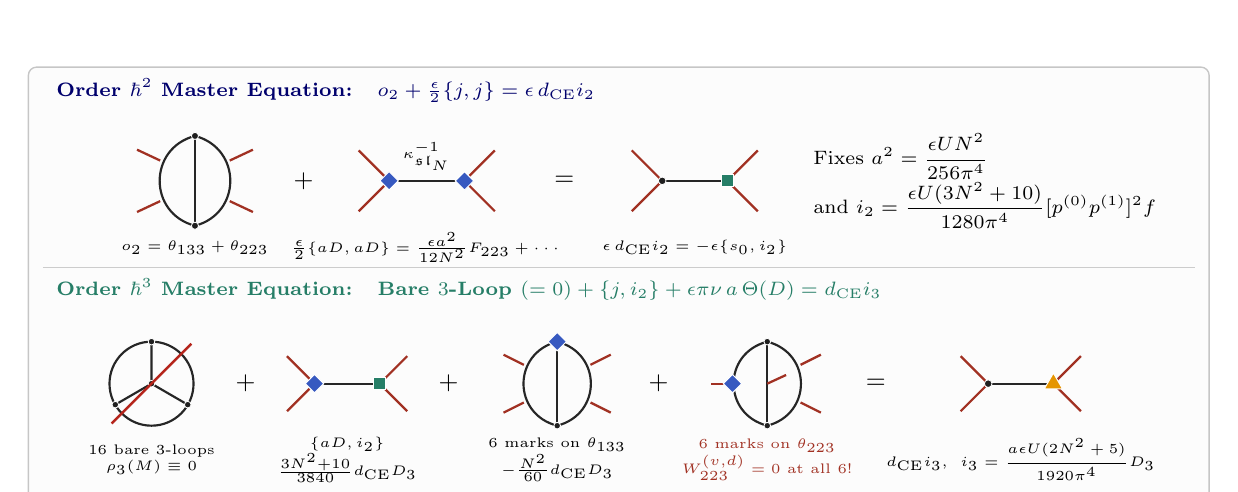
\begin{tikzpicture}[scale=0.92]
  \draw[rounded corners=3pt, draw=gray!45, fill=gray!2, line width=0.5pt] (-8.15,-3.25) rectangle (8.15,2.75);

  % Top row: Order hbar^2 QME
  \node[font=\scriptsize\bfseries, anchor=west, text=NavyBlue!85!black] at (-7.9,2.42) {Order $\hbar^2$ Master Equation:\quad $o_2 + \frac{\epsilon}{2}\{j, j\} = \epsilon\,d_{\mathrm{CE}} i_2$};

  % Bare theta sum
  \begin{scope}[xshift=-5.85cm, yshift=1.18cm]
    \draw[prop] (0,0.62) -- (0,-0.62);
    \draw[prop] (0,0.62) .. controls (-0.65,0.45) and (-0.65,-0.45) .. (0,-0.62);
    \draw[prop] (0,0.62) .. controls ( 0.65,0.45) and ( 0.65,-0.45) .. (0,-0.62);
    \draw[extleg] (-0.48,0.28) -- ++(-0.32,0.15);
    \draw[extleg] (-0.48,-0.28) -- ++(-0.32,-0.15);
    \draw[extleg] ( 0.48,0.28) -- ++( 0.32,0.15);
    \draw[extleg] ( 0.48,-0.28) -- ++( 0.32,-0.15);
    \filldraw[v0] (0,0.62) circle (1.4pt); \filldraw[v0] (0,-0.62) circle (1.4pt);
    \node[font=\tiny] at (0,-0.92) {$o_2 = \theta_{133} + \theta_{223}$};
  \end{scope}

  \node[font=\small\bfseries] at (-4.35,1.18) {$+$};

  % Tree 1/2 {J_1, J_1}
  \begin{scope}[xshift=-2.65cm, yshift=1.18cm]
    \coordinate (u1) at (-0.52,0); \coordinate (u2) at (0.52,0);
    \draw[prop] (u1) -- node[above, font=\tiny] {$\kappa^{-1}_{\fsl_N}$} (u2);
    \draw[extleg] (u1) -- ++(-0.42, 0.42);
    \draw[extleg] (u1) -- ++(-0.42,-0.42);
    \draw[extleg] (u2) -- ++( 0.42, 0.42);
    \draw[extleg] (u2) -- ++( 0.42,-0.42);
    \node[vj1] at (u1) {}; \node[vj1] at (u2) {};
    \node[font=\tiny] at (0,-0.92) {$\frac{\epsilon}{2}\{aD, aD\} = \frac{\epsilon a^2}{12N^2}F_{223} + \cdots$};
  \end{scope}

  \node[font=\small\bfseries] at (-0.75,1.18) {$=$};

  % Coboundary d i_2
  \begin{scope}[xshift=1.05cm, yshift=1.18cm]
    \coordinate (w1) at (-0.45,0); \coordinate (w2) at (0.45,0);
    \draw[prop] (w1) -- (w2);
    \draw[extleg] (w1) -- ++(-0.42, 0.42);
    \draw[extleg] (w1) -- ++(-0.42,-0.42);
    \draw[extleg] (w2) -- ++( 0.42, 0.42);
    \draw[extleg] (w2) -- ++( 0.42,-0.42);
    \filldraw[v0] (w1) circle (1.5pt); \node[vi2] at (w2) {};
    \node[font=\tiny] at (0,-0.92) {$\epsilon\,d_{\mathrm{CE}}i_2 = -\epsilon\{s_0, i_2\}$};
  \end{scope}

  \node[font=\scriptsize, align=left, anchor=west] at (2.55,1.18) {Fixes $a^2 = \dfrac{\epsilon UN^2}{256\pi^4}$\\and $i_2 = \dfrac{\epsilon U(3N^2+10)}{1280\pi^4}[p^{(0)}p^{(1)}]^2 f$};

  % Divider
  \draw[gray!40, line width=0.45pt] (-7.95,-0.02) -- (7.95,-0.02);

  % Bottom row: Order hbar^3 QME
  \node[font=\scriptsize\bfseries, anchor=west, text=PineGreen!85!black] at (-7.9,-0.32) {Order $\hbar^3$ Master Equation:\quad $\text{Bare }3\text{-Loop }(=0) + \{j, i_2\} + \epsilon\pi\nu\,a\,\Theta(D) = d_{\mathrm{CE}} i_3$};

  % Bare 3-loop K_4 (=0)
  \begin{scope}[xshift=-6.45cm, yshift=-1.62cm]
    \draw[prop] (0,0) circle (0.58cm);
    \draw[prop] (0,0.58) -- (0,0) -- (-0.50,-0.29);
    \draw[prop] (0,0) -- (0.50,-0.29);
    \filldraw[v0] (0,0) circle (1.3pt); \filldraw[v0] (0,0.58) circle (1.3pt);
    \filldraw[v0] (-0.50,-0.29) circle (1.3pt); \filldraw[v0] (0.50,-0.29) circle (1.3pt);
    \draw[BrickRed, line width=0.9pt] (-0.55,-0.55) -- (0.55,0.55);
    \node[font=\tiny, align=center] at (0,-1.05) {$16$ bare $3$-loops\\$\rho_3(M) \equiv 0$};
  \end{scope}

  \node[font=\small\bfseries] at (-5.15,-1.62) {$+$};

  % Tree {J_1, I_2}
  \begin{scope}[xshift=-3.75cm, yshift=-1.62cm]
    \coordinate (t1) at (-0.45,0); \coordinate (t2) at (0.45,0);
    \draw[prop] (t1) -- (t2);
    \draw[extleg] (t1) -- ++(-0.38, 0.38); \draw[extleg] (t1) -- ++(-0.38,-0.38);
    \draw[extleg] (t2) -- ++( 0.38, 0.38); \draw[extleg] (t2) -- ++( 0.38,-0.38);
    \node[vj1] at (t1) {}; \node[vi2] at (t2) {};
    \node[font=\tiny, align=center] at (0,-1.05) {$\{aD, i_2\}$\\$\frac{3N^2+10}{3840}d_{\mathrm{CE}}D_3$};
  \end{scope}

  \node[font=\small\bfseries] at (-2.35,-1.62) {$+$};

  % Marked theta_133 (hub + leg = 6 placements)
  \begin{scope}[xshift=-0.85cm, yshift=-1.62cm]
    \draw[prop] (0,0.58) -- (0,-0.58);
    \draw[prop] (0,0.58) .. controls (-0.62,0.42) and (-0.62,-0.42) .. (0,-0.58);
    \draw[prop] (0,0.58) .. controls ( 0.62,0.42) and ( 0.62,-0.42) .. (0,-0.58);
    \draw[extleg] (-0.46,0.26) -- ++(-0.28,0.14); \draw[extleg] (-0.46,-0.26) -- ++(-0.28,-0.14);
    \draw[extleg] ( 0.46,0.26) -- ++( 0.28,0.14); \draw[extleg] ( 0.46,-0.26) -- ++( 0.28,-0.14);
    \node[vj1] at (0,0.58) {}; \filldraw[v0] (0,-0.58) circle (1.3pt);
    \node[font=\tiny, align=center] at (0,-1.05) {$6$ marks on $\theta_{133}$\\$-\frac{N^2}{60}d_{\mathrm{CE}}D_3$};
  \end{scope}

  \node[font=\small\bfseries] at (0.55,-1.62) {$+$};

  % Marked theta_223 (all 6 placements = 0!)
  \begin{scope}[xshift=2.05cm, yshift=-1.62cm]
    \draw[prop] (0,0.58) -- (0,-0.58);
    \draw[prop] (0,0.58) .. controls (-0.62,0.42) and (-0.62,-0.42) .. (0,-0.58);
    \draw[prop] (0,0.58) .. controls ( 0.62,0.42) and ( 0.62,-0.42) .. (0,-0.58);
    \draw[extleg] (-0.48,0) -- ++(-0.30,0); \draw[extleg] (0,0) -- ++(0.26,0.12);
    \draw[extleg] ( 0.46,0.26) -- ++( 0.28,0.14); \draw[extleg] ( 0.46,-0.26) -- ++( 0.28,-0.14);
    \node[vj1] at (-0.48,0) {}; \filldraw[v0] (0,0.58) circle (1.3pt); \filldraw[v0] (0,-0.58) circle (1.3pt);
    \node[font=\tiny, align=center, text=BrickRed!85!black] at (0,-1.05) {$6$ marks on $\theta_{223}$\\$W^{(v,d)}_{223} = 0$ at all $6$!};
  \end{scope}

  \node[font=\small\bfseries] at (3.55,-1.62) {$=$};

  % d i_3
  \begin{scope}[xshift=5.55cm, yshift=-1.62cm]
    \coordinate (s1) at (-0.45,0); \coordinate (s2) at (0.45,0);
    \draw[prop] (s1) -- (s2);
    \draw[extleg] (s1) -- ++(-0.38, 0.38); \draw[extleg] (s1) -- ++(-0.38,-0.38);
    \draw[extleg] (s2) -- ++( 0.38, 0.38); \draw[extleg] (s2) -- ++( 0.38,-0.38);
    \filldraw[v0] (s1) circle (1.5pt); \node[vi3] at (s2) {};
    \node[font=\tiny, align=center] at (0,-1.05) {$d_{\mathrm{CE}}i_3$,\ \ $i_3 = \dfrac{a\epsilon U(2N^2+5)}{1920\pi^4}D_3$};
  \end{scope}
\end{tikzpicture}
\caption{Diagrammatic master equations at $\hbar^2$ (top) and $\hbar^3$ (bottom). At $\hbar^3$, all $16$ bare three-loop graphs vanish by $\rho_3=0$, and all $6$ placements of $J_1$ on $\theta(2,2,3)$ vanish vertex by vertex.}
\label{fig:order2-order3-qme}
\end{figure}

\begin{proposition}[First three quantum counterterms and $N=2$ specialization]
\label{prop:i1-i2-i3}
On $\fg = \fsl_N$ ($\kappa = \tr$) with $D_3(X_0,X_1,X_2) := [p^{(0)}p^{(1)}]^3\tr(X_0\{X_1,X_2\})$:
\begin{enumerate}[label=(\alph*),leftmargin=*]
  \item \textbf{Unique $j, i_2, i_3$ for $N \ge 3$:} The shuffle bracket satisfies $\frac{1}{2}\{D, D\} = \frac{1}{12N^2}F_{223} + \frac{N^2+4}{2N^2}\beta$, forcing $j = a D$ with $a^2 = \frac{\epsilon U N^2}{256\pi^4}$ and $i_2 = \frac{\epsilon U(3N^2+10)}{1280\pi^4}[p^{(0)}p^{(1)}]^2 f$. At $\hbar^3$, $\{D, [p^{(0)}p^{(1)}]^2 f\} = \frac{1}{3}d_{\mathrm{CE}}D_3$ and the $12$ single-$D$-marked theta diagrams evaluate to $\Theta(D) = -\frac{N^2}{60}d_{\mathrm{CE}}D_3$, yielding $d_{\mathrm{CE}}i_3 = \{j,i_2\} + \epsilon\pi\nu\,a\,\Theta(D)$ with unique primitive $i_3 = \frac{a\epsilon U(2N^2+5)}{1920\pi^4}D_3$.
  \item \textbf{Two-branch $\mathsf{C}$-symmetry and $N = 2$ specialization:} Charge conjugation $\mathsf{C}(X) := -X^{\mathsf{T}}$ preserves $\tr$ and $f$ while reversing $D \mapsto -D$, exchanging $+a \leftrightarrow -a$ (fixing even $I_{2k}$ and negating odd $I_{2k+1}$). At $N = 2$, $X_1 X_2 + X_2 X_1 = \tr(X_1 X_2)\mathbf{1}_2$ gives $\tr(X_0\{X_1,X_2\}) = 0$, so both branches specialize to $j = 0$, $i_2|_{\fsl_2} = \frac{11\epsilon U}{640\pi^4}[p^{(0)}p^{(1)}]^2 f$, and $i_3 = 0$.
\end{enumerate}
\end{proposition}

\begin{proof}\leavevmode\par\vspace{2pt}
\begin{proofpart}{Proof of (a): Unique counterterms $j, i_2, i_3$ for $N \ge 3$}
Contracting $D$ with itself via~\eqref{eq:traceless-completeness} gives $d_{\mathrm{CE}}i_2 = (\frac{a^2}{12N^2} + \frac{\epsilon\pi\nu}{48})F_{223} + (\frac{a^2(N^2+4)}{2N^2} - \frac{\epsilon\pi\nu N^2}{40})\beta$; since $[F_{223}] \neq 0$ for $N \ge 3$, $a^2 = -\frac{\epsilon\pi\nu N^2}{4} = \frac{\epsilon U N^2}{256\pi^4}$, and substituting $a^2$ into the $\beta$ coefficient gives $\frac{\epsilon U}{512\pi^4}(N^2+4) + \frac{\epsilon U}{2560\pi^4}N^2 = \frac{\epsilon U(3N^2+10)}{1280\pi^4}$. At $\hbar^3$, summing $\frac{3N^2+10}{3840} + \frac{N^2}{3840} = \frac{4N^2+10}{3840} = \frac{2N^2+5}{1920}$ gives $i_3$ (\zkcard{fived-cs-sl3-counterterm-spotcheck} verifies $N=3$: $\frac{37}{1280\pi^4}$ and $\frac{23}{1920\pi^4}$).
\end{proofpart}
\begin{proofpart}{Proof of (b): Charge conjugation and $N = 2$ specialization}
Applying $\mathsf{C}(X) = -X^{\mathsf{T}}$ preserves $[X_1,X_2]$ and reverses $\{X_1,X_2\} \mapsto -\{X_1,X_2\}$, pairing $+a$ with $-a$. At $N = 2$, $X_1 X_2 + X_2 X_1 = \tr(X_1 X_2)\mathbf{1}_2$ kills $D$ and $D_3$, and setting $N = 2$ in $\frac{3N^2+10}{1280} = \frac{22}{1280} = \frac{11}{640}$ yields $i_2|_{\fsl_2}$.\qedhere
\end{proofpart}
\end{proof}

% ============================================================================
\section{All-Order Quantization and Complete 50-Graph Fourth-Order Calculation}
\label{sec:allorders-hbar4}
% ============================================================================

\subsection{Polygon bar-duality, two-trace coprimality, and all-order $\fsl_N$ theorem}
\label{subsec:all-orders}

In the formal trace algebra of traceless matrices (which agrees with invariant tensors of $\fsl_N$ in arities $\le 5$ for all $N \ge 5$), $d_{\mathrm{CE}}$ inserts a commutator and preserves the number of cyclic traces.

\begin{proposition}[Complete formal obstruction cohomology at degree $2w$]
\label{prop:all-order-h4}
For every integer $w \ge 2$, the formal trace complex of $\fsl_N$ satisfies
\begin{equation}
\label{eq:all-order-h3-h4}
H^3(C^0_{\fsl_N})_{\deg=2w} = 0, \qquad
H^4(C^0_{\fsl_N})_{\deg=2w} \cong \Sym^{2w-4}(\mathbb{C}^2), \qquad
\dim\!\big(H^4(C^0_{\fsl_N})_{\deg=2w}\big)^{\SL_2(\mathbb{C})} = \delta_{w,2},
\end{equation}
where $H^4_{\deg=2w}$ is spanned by double-trace cocycles $[p^{(0)}P][p^{(2)}P]h(P)\tr(X_0 X_1)\tr(X_2 X_3)$ ($P := p^{(0)}+p^{(1)}$, $\deg h = 2w - 4$) and their signed permutations.
\end{proposition}

\begin{proof}\leavevmode\par\vspace{2pt}
\begin{proofpart}{Single-trace summand: polygon bar-duality and Connes' sequence}
Representing $\sum_{\substack{q=0\\\mathrm{sides}}}^{k-1} p^{(q)} = 0$ on $\tr(X_0\cdots X_{k-1})$ as polygon edge increments $p^{(q)} = x_{q+1} - x_q$ ($x_k = x_0$), commutator insertion merges adjacent edges and deletes the shared vertex. Before cyclicity ($j = k - 1$), this deletion differential in fixed polynomial degree $m$ is the graded dual of the reduced bar resolution of $\mathbb{C}[y_1,y_2]$, whose Koszul resolution gives $HH^j_m = \Lambda^j(\mathbb{C}^2)\delta_{m,j}$ ($0 \le j \le 2$), hence $HH^j_m = 0$ for all $m > 2$! Connes' exact sequence $HC^{j-2}_m \to HC^j_m \to HH^j_m$ inducts from $j < 0$ to prove $HC^j_m = 0$ for all $m > 2$ ($2w \ge 4 > 2$), killing all single-trace $H^3$ and $H^4$ classes.
\end{proofpart}
\begin{proofpart}{Double-trace summand: Cauchy linearity and coprime determinants}
Since $\tr(X)=0$, arity $3$ has zero two-trace words, while arity $4$ has word type $(01)(23)$ on momenta $(r, P-r, q, -P-q)$ with coefficient $F(r,q,P)$ obeying $F(P-r,q,P) = -F(r,q,P) = F(r,-P-q,P)$ and $F(q,r,-P) = F(r,q,P)$. Vanishing of $d_{\mathrm{CE}}F$ on $\tr(X_0 X_1 X_2)\tr(X_3 X_4)$ reads $F(r,q,P) + F(s,q,P) + F(P-r-s,q,P) = 0 \Longleftrightarrow F(r+s,q,P) = F(r,q,P) + F(s,q,P)$, forcing $F$ to be linear in $r$ and to vanish at $r = P$ ($2F(P,q,P) = 0$)! Because $P_1, P_2$ are coprime in $\mathbb{C}[P_1,P_2]$, any linear functional in $r$ killing $P$ is a polynomial multiple of $[rP]$. Repeating in $q$ yields $F(r,q,P) = [rP][qP]h(P)$ ($\deg h = 2w - 4$), isomorphic as an $\SL_2(\mathbb{C})$-module to $\Sym^{2w-4}(\mathbb{C}^2)$ (spin $w - 2$, whose $\SL_2$-invariant subspace is nonzero solely at $w - 2 = 0$).\qedhere
\end{proofpart}
\end{proof}

\begin{theorem}[All-order formal quantization, specialization to $N \ge 2$, and probe extraction]
\label{thm:all-orders-traceless}
For each root $a$ of $a^2 = \frac{\epsilon U N^2}{256\pi^4}$ on $\fsl_N$ ($\kappa = \tr$), there exists a unique formal $\mathrm{U}(2)$-equivariant sequence of invariant cubic counterterms $I_w = F_{i_w} \in \Vht^0$ ($w \ge 2$),
\begin{equation}
\label{eq:iw-ansatz}
i_w = c_w(N)\,[p^{(0)}p^{(1)}]^w \begin{cases} \tr(X_0[X_1,X_2]), & w\text{ even},\\ \tr(X_0\{X_1,X_2\}), & w\text{ odd}, \end{cases} \qquad c_w(N) \in \mathbb{C}[N, N^{-1}],
\end{equation}
solving the local heat-kernel QME to all orders $\hbar^w$ in the formal trace algebra and specializing to a valid QME solution at every integer $N \ge 2$. Evaluating the order-$w$ cochain equation on $(X_0,X_1,X_2,X_3) = (E_{12}, E_{23}, E_{34}, E_{41})$ ($N \ge 4$) at momenta $(p^{(0)},p^{(1)},p^{(2)},p^{(3)}) = ((1,0),(0,1),(1,1),(-2,-2))$ divides by the exact nonzero integer
\begin{equation}
\label{eq:probe-denominator}
-[p^{(2)}p^{(3)}]^w + [p^{(1)}p^{(2)}]^w + [p^{(3)}p^{(0)}]^w - [p^{(0)}p^{(1)}]^w = 2^w + (-1)^w - 1 = \begin{cases} 2^w, & w\text{ even},\\ 2^w - 2, & w\text{ odd}. \end{cases}
\end{equation}
\end{theorem}

\begin{proof}
Suppose $I_2,\dots,I_{w-1}$ solve the QME below order $w \ge 3$. By the finite-scale BV Bianchi identity~\cite{CostelloBV,WW} (\zkcard{costello-counterterms-qme-tower}) and Lemma~\ref{lem:full-wedge-contacts}, the order-$w$ obstruction $o_w$ lies in $C^{0,4}_{\fsl_N}$ at bidegree $(w,w)$, is $d_{\mathrm{CE}}$-closed, and is $\SL_2(\mathbb{C})$-invariant; Proposition~\ref{prop:all-order-h4} gives $[o_w] = 0$ and $H^3_{\deg=2w} = 0$, so $d_{\mathrm{CE}}$ is injective on the $1$-dimensional cubic space~\eqref{eq:iw-ansatz}. Fixing $a/N$ constant,~\eqref{eq:traceless-completeness} places every graph contraction in $\mathbb{C}[N,N^{-1}]$, while inverting $d_{\mathrm{CE}}$ on its image introduces purely rational $N$-independent denominators; evaluation on $N\times N$ traceless matrices commutes with $d_{\mathrm{CE}}$ and contractions for every $N \ge 2$. Direct substitution $[p^{(2)}p^{(3)}] = 0$, $[p^{(1)}p^{(2)}] = -1$, $[p^{(3)}p^{(0)}] = 2$, $[p^{(0)}p^{(1)}] = 1$ yields~\eqref{eq:probe-denominator}.
\end{proof}

\subsection{Five six-vertex cores, SP bubble symmetry, and marked $\hbar^4$ diagrams}
\label{subsec:fourloop-cores}

Fix $\epsilon U = +1$, so $(\epsilon\pi\nu)^2 = \frac{1}{4096\pi^8}$ and the probe denominator~\eqref{eq:probe-denominator} at $w = 4$ equals $2^4 = 16$. By~\eqref{eq:tight-5d-count} at $n = 4$, a tight bare cubic four-loop graph has $|V| = 10$ vertices, $|E| = 13$ internal edges, and $4$ bivalent external vertices (internal degree $1$ or cut vertices violate $2|E_S|\le 3|V_S|-4$ on the complement). Suppressing the $4$ bivalent vertices leaves a loopless biconnected $6$-vertex cubic multigraph of multiplicity $\le 2$. Exhaustive enumeration~\cite[\S6.2]{RepoAllOrders} produces $550$ labelled graphs grouped into \textbf{five unlabelled $6$-vertex cores}, drawn in Figure~\ref{fig:five-sixvertex-cores}.

\begin{figure}[H]
\centering
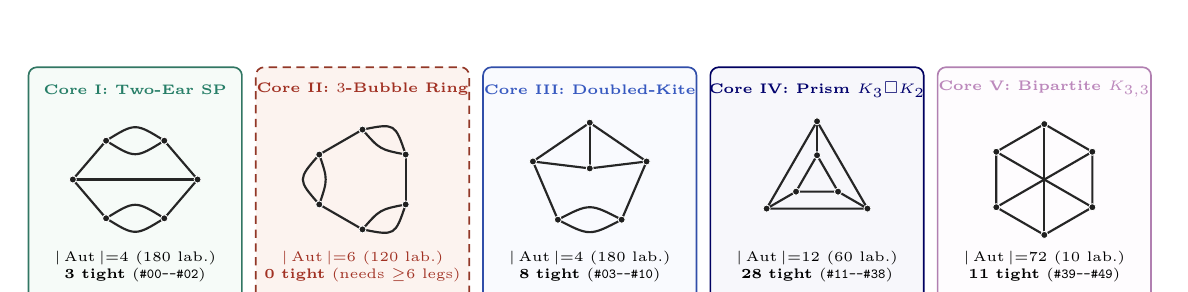
\begin{tikzpicture}[scale=0.88]
  % Core I: Two-Ear SP
  \begin{scope}[xshift=-6.56cm]
    \draw[rounded corners=3pt, draw=PineGreen!75!black, fill=PineGreen!3, line width=0.6pt] (-1.54,-1.68) rectangle (1.54,1.70);
    \node[font=\tiny\bfseries, text=PineGreen!85!black] at (0,1.38) {Core I: Two-Ear SP};
    \coordinate (a0) at (-0.9,0.08); \coordinate (a3) at (0.9,0.08);
    \coordinate (a1) at (-0.42,0.64); \coordinate (a2) at (0.42,0.64);
    \coordinate (a5) at (-0.42,-0.48); \coordinate (a4) at (0.42,-0.48);
    \draw[prop] (a0) -- (a3);
    \draw[prop] (a0) -- (a1); \draw[prop] (a2) -- (a3);
    \draw[prop] (a1) .. controls (0,0.90) .. (a2);
    \draw[prop] (a1) .. controls (0,0.38) .. (a2);
    \draw[prop] (a0) -- (a5); \draw[prop] (a4) -- (a3);
    \draw[prop] (a5) .. controls (0,-0.74) .. (a4);
    \draw[prop] (a5) .. controls (0,-0.22) .. (a4);
    \foreach \pt in {a0,a1,a2,a3,a4,a5} \filldraw[v0] (\pt) circle (1.45pt);
    \node[font=\tiny, align=center] at (0,-1.18) {$|\Aut|{=}4$ ($180$ lab.)\\$\mathbf{3}$ \textbf{tight} (\texttt{\#00--\texttt{\#02}})};
  \end{scope}

  % Core II: 3-Bubble Necklace (0 tight!)
  \begin{scope}[xshift=-3.28cm]
    \draw[rounded corners=3pt, draw=BrickRed!75!black, fill=BrickRed!4, line width=0.6pt, densely dashed] (-1.54,-1.68) rectangle (1.54,1.70);
    \node[font=\tiny\bfseries, text=BrickRed!85!black] at (0,1.38) {Core II: $3$-Bubble Ring};
    \begin{scope}[yshift=0.08cm]
      \foreach \k/\ang in {b0/90, b1/30, b3/330, b5/270, b4/210, b2/150}
        \coordinate (\k) at ({\ang}:0.72cm);
      \draw[prop] (b0) .. controls (60:0.94cm) .. (b1);
      \draw[prop] (b0) .. controls (60:0.50cm) .. (b1);
      \draw[prop] (b1) -- (b3);
      \draw[prop] (b3) .. controls (300:0.94cm) .. (b5);
      \draw[prop] (b3) .. controls (300:0.50cm) .. (b5);
      \draw[prop] (b5) -- (b4);
      \draw[prop] (b4) .. controls (180:0.94cm) .. (b2);
      \draw[prop] (b4) .. controls (180:0.50cm) .. (b2);
      \draw[prop] (b2) -- (b0);
      \foreach \pt in {b0,b1,b2,b3,b4,b5} \filldraw[v0] (\pt) circle (1.45pt);
    \end{scope}
    \node[font=\tiny, align=center, text=BrickRed!85!black] at (0,-1.18) {$|\Aut|{=}6$ ($120$ lab.)\\$\mathbf{0}$ \textbf{tight} (needs ${\ge}6$ legs)};
  \end{scope}

  % Core III: Doubled-Kite
  \begin{scope}[xshift=0cm]
    \draw[rounded corners=3pt, draw=RoyalBlue!75!black, fill=RoyalBlue!3, line width=0.6pt] (-1.54,-1.68) rectangle (1.54,1.70);
    \node[font=\tiny\bfseries, text=RoyalBlue!85!black] at (0,1.38) {Core III: Doubled-Kite};
    \begin{scope}[yshift=0.08cm]
      \coordinate (c5) at (0,0.16); \coordinate (c1) at (0,0.82);
      \coordinate (c0) at (-0.82,0.26); \coordinate (c2) at (0.82,0.26);
      \coordinate (c4) at (-0.46,-0.58); \coordinate (c3) at (0.46,-0.58);
      \draw[prop] (c0) -- (c1) -- (c2) -- (c3); \draw[prop] (c0) -- (c4);
      \draw[prop] (c0) -- (c5); \draw[prop] (c1) -- (c5); \draw[prop] (c2) -- (c5);
      \draw[prop] (c4) .. controls (0,-0.34) .. (c3);
      \draw[prop] (c4) .. controls (0,-0.82) .. (c3);
      \foreach \pt in {c0,c1,c2,c3,c4,c5} \filldraw[v0] (\pt) circle (1.45pt);
    \end{scope}
    \node[font=\tiny, align=center] at (0,-1.18) {$|\Aut|{=}4$ ($180$ lab.)\\$\mathbf{8}$ \textbf{tight} (\texttt{\#03--\texttt{\#10}})};
  \end{scope}

  % Core IV: Triangular Prism
  \begin{scope}[xshift=3.28cm]
    \draw[rounded corners=3pt, draw=NavyBlue!75!black, fill=NavyBlue!3, line width=0.6pt] (-1.54,-1.68) rectangle (1.54,1.70);
    \node[font=\tiny\bfseries, text=NavyBlue!85!black] at (0,1.38) {Core IV: Prism $K_3{\square}K_2$};
    \begin{scope}[yshift=0.08cm]
      \coordinate (d0) at (90:0.35cm); \coordinate (d3) at (210:0.35cm); \coordinate (d2) at (330:0.35cm);
      \coordinate (d1) at (90:0.84cm); \coordinate (d4) at (210:0.84cm); \coordinate (d5) at (330:0.84cm);
      \draw[prop] (d0) -- (d3) -- (d2) -- cycle;
      \draw[prop] (d1) -- (d4) -- (d5) -- cycle;
      \draw[prop] (d0) -- (d1); \draw[prop] (d3) -- (d4); \draw[prop] (d2) -- (d5);
      \foreach \pt in {d0,d1,d2,d3,d4,d5} \filldraw[v0] (\pt) circle (1.45pt);
    \end{scope}
    \node[font=\tiny, align=center] at (0,-1.18) {$|\Aut|{=}12$ ($60$ lab.)\\$\mathbf{28}$ \textbf{tight} (\texttt{\#11--\texttt{\#38}})};
  \end{scope}

  % Core V: Non-planar K_{3,3}
  \begin{scope}[xshift=6.56cm]
    \draw[rounded corners=3pt, draw=Plum!80!black, fill=Plum!3, line width=0.6pt] (-1.54,-1.68) rectangle (1.54,1.70);
    \node[font=\tiny\bfseries, text=Plum!85!black] at (0,1.38) {Core V: Bipartite $K_{3,3}$};
    \begin{scope}[yshift=0.08cm]
      \foreach \k in {0,1,2,3,4,5} \coordinate (e\k) at ({90-60*\k}:0.80cm);
      \draw[prop] (e0) -- (e1) -- (e2) -- (e3) -- (e4) -- (e5) -- cycle;
      \draw[prop] (e0) -- (e3);
      \draw[prop] (e1) .. controls (0.14,0.08) .. (e4);
      \draw[prop] (e2) .. controls (-0.14,0.08) .. (e5);
      \foreach \k in {0,1,2,3,4,5} \filldraw[v0] (e\k) circle (1.45pt);
    \end{scope}
    \node[font=\tiny, align=center] at (0,-1.18) {$|\Aut|{=}72$ ($10$ lab.)\\$\mathbf{11}$ \textbf{tight} (\texttt{\#39--\texttt{\#49}})};
  \end{scope}
\end{tikzpicture}
\caption{The five loopless biconnected $6$-vertex cubic multigraph cores ($180+120+180+60+10 = 550$ labelled cores). Each parallel $2$-edge bubble $(u,v)$ violates $2|E_S|\le 3|V_S|-4$ ($4 > 2$) unless subdivided by at least two external vertices; hence Core~II ($3$ bubbles, needing $\ge 6 > 4$ subdivisions) yields $0$ tight graphs, leaving $3+8+28+11 = 50$ bare four-loop diagrams.}
\label{fig:five-sixvertex-cores}
\end{figure}

Before displaying all $50$ bare diagrams, Figure~\ref{fig:fourloop-sp-and-marked} illustrates two striking graphical mechanisms at $\hbar^4$: first, among the three series--parallel graphs \texttt{\#00}--\texttt{\#02}, \textbf{solely \texttt{\#00} is nonzero} ($K_1 = K_2 = 0$ identically by $(2,2)$-bubble tail symmetry!); second, the tree brackets $\{D, D_3\} = 10$ and $\frac{1}{2}\{[p^{(0)}p^{(1)}]^2 f, [p^{(0)}p^{(1)}]^2 f\} = -4$ combine with single-$I_2$-marked and doubly-$J_1$-marked theta diagrams into the purely rational piece $(\epsilon\pi\nu)^2\frac{21221N^4 + 85304N^2 + 192480}{3628800}$ (Table~\ref{tab:marked-theta-h4}).

\begin{figure}[H]
\centering
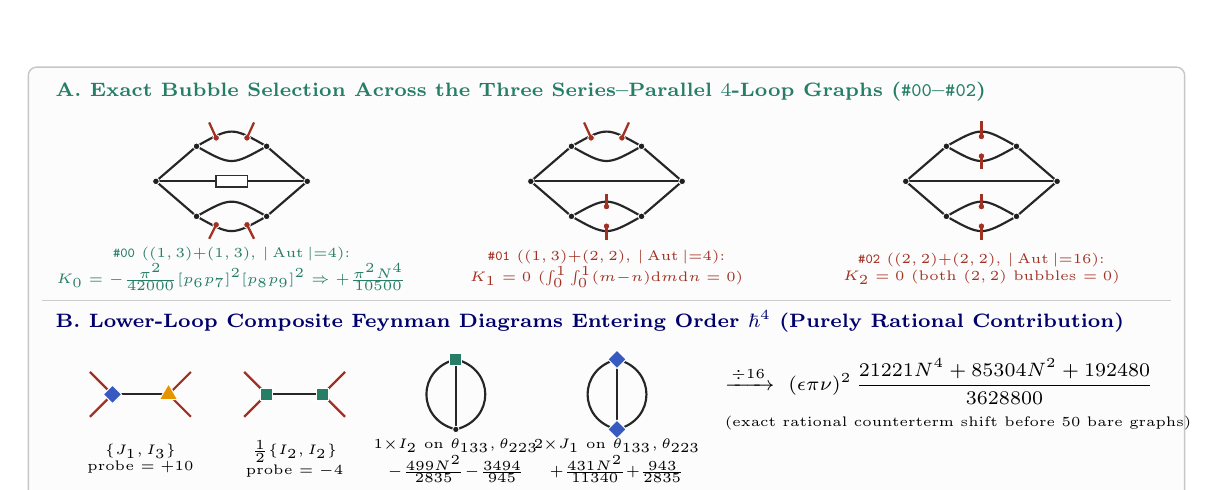
\begin{tikzpicture}[scale=0.89]
  \draw[rounded corners=3pt, draw=gray!45, fill=gray!2, line width=0.5pt] (-8.25,-3.32) rectangle (8.25,2.85);

  % Top row: 3 SP graphs #00, #01, #02 with bubble mechanism
  \node[font=\scriptsize\bfseries, anchor=west, text=PineGreen!85!black] at (-8.00,2.50) {A. Exact Bubble Selection Across the Three Series--Parallel $4$-Loop Graphs (\texttt{\#00}--\texttt{\#02})};

  % #00: (1,3) + (1,3)
  \begin{scope}[xshift=-5.35cm, yshift=1.22cm]
    \coordinate (g0) at (-1.08,0); \coordinate (g3) at (1.08,0);
    \coordinate (g1) at (-0.50,0.50); \coordinate (g2) at (0.50,0.50);
    \coordinate (g5) at (-0.50,-0.50); \coordinate (g4) at (0.50,-0.50);
    \draw[prop] (g0) -- node[iecres, scale=0.65] {} (g3);
    \draw[prop] (g0) -- (g1); \draw[prop] (g2) -- (g3);
    \draw[prop] (g1) .. controls (0,0.78) .. (g2);
    \draw[prop] (g1) .. controls (0,0.22) .. (g2);
    \draw[prop] (g0) -- (g5); \draw[prop] (g4) -- (g3);
    \draw[prop] (g5) .. controls (0,-0.78) .. (g4);
    \draw[prop] (g5) .. controls (0,-0.22) .. (g4);
    % (1,3) legs on outer arcs
    \filldraw[vbiv] (-0.22,0.62) circle (1.35pt); \draw[extleg] (-0.22,0.62) -- ++(-0.10,0.22);
    \filldraw[vbiv] ( 0.22,0.62) circle (1.35pt); \draw[extleg] ( 0.22,0.62) -- ++( 0.10,0.22);
    \filldraw[vbiv] (-0.22,-0.62) circle (1.35pt); \draw[extleg] (-0.22,-0.62) -- ++(-0.10,-0.20);
    \filldraw[vbiv] ( 0.22,-0.62) circle (1.35pt); \draw[extleg] ( 0.22,-0.62) -- ++( 0.10,-0.20);
    \foreach \pt in {g0,g1,g2,g3,g4,g5} \filldraw[v0] (\pt) circle (1.35pt);
    \node[font=\tiny, align=center, text=PineGreen!85!black] at (0,-1.25) {\texttt{\#00} ($(1,3){+}(1,3)$, $|\Aut|{=}4$):\\$K_0 = -\frac{\pi^2}{42000}[p_6 p_7]^2[p_8 p_9]^2 \Rightarrow +\frac{\pi^2 N^4}{10500}$};
  \end{scope}

  % #01: (1,3) + (2,2) = 0
  \begin{scope}[xshift=0cm, yshift=1.22cm]
    \coordinate (h0) at (-1.08,0); \coordinate (h3) at (1.08,0);
    \coordinate (h1) at (-0.50,0.50); \coordinate (h2) at (0.50,0.50);
    \coordinate (h5) at (-0.50,-0.50); \coordinate (h4) at (0.50,-0.50);
    \draw[prop] (h0) -- (h3);
    \draw[prop] (h0) -- (h1); \draw[prop] (h2) -- (h3);
    \draw[prop] (h1) .. controls (0,0.78) .. (h2);
    \draw[prop] (h1) .. controls (0,0.22) .. (h2);
    \draw[prop] (h0) -- (h5); \draw[prop] (h4) -- (h3);
    \draw[prop] (h5) .. controls (0,-0.78) .. (h4);
    \draw[prop] (h5) .. controls (0,-0.22) .. (h4);
    \filldraw[vbiv] (-0.22,0.62) circle (1.35pt); \draw[extleg] (-0.22,0.62) -- ++(-0.10,0.22);
    \filldraw[vbiv] ( 0.22,0.62) circle (1.35pt); \draw[extleg] ( 0.22,0.62) -- ++( 0.10,0.22);
    \filldraw[vbiv] (0,-0.64) circle (1.35pt); \draw[extleg] (0,-0.64) -- ++(0,-0.20);
    \filldraw[vbiv] (0,-0.36) circle (1.35pt); \draw[extleg] (0,-0.36) -- ++(0,0.18);
    \foreach \pt in {h0,h1,h2,h3,h4,h5} \filldraw[v0] (\pt) circle (1.35pt);
    \node[font=\tiny, align=center, text=BrickRed!85!black] at (0,-1.25) {\texttt{\#01} ($(1,3){+}(2,2)$, $|\Aut|{=}4$):\\$K_1 = 0$ ($\int_0^1\int_0^1(m{-}n)\dd m\dd n = 0$)};
  \end{scope}

  % #02: (2,2) + (2,2) = 0
  \begin{scope}[xshift=5.35cm, yshift=1.22cm]
    \coordinate (k0) at (-1.08,0); \coordinate (k3) at (1.08,0);
    \coordinate (k1) at (-0.50,0.50); \coordinate (k2) at (0.50,0.50);
    \coordinate (k5) at (-0.50,-0.50); \coordinate (k4) at (0.50,-0.50);
    \draw[prop] (k0) -- (k3);
    \draw[prop] (k0) -- (k1); \draw[prop] (k2) -- (k3);
    \draw[prop] (k1) .. controls (0,0.78) .. (k2);
    \draw[prop] (k1) .. controls (0,0.22) .. (k2);
    \draw[prop] (k0) -- (k5); \draw[prop] (k4) -- (k3);
    \draw[prop] (k5) .. controls (0,-0.78) .. (k4);
    \draw[prop] (k5) .. controls (0,-0.22) .. (k4);
    \filldraw[vbiv] (0, 0.64) circle (1.35pt); \draw[extleg] (0, 0.64) -- ++(0, 0.22);
    \filldraw[vbiv] (0, 0.36) circle (1.35pt); \draw[extleg] (0, 0.36) -- ++(0,-0.18);
    \filldraw[vbiv] (0,-0.64) circle (1.35pt); \draw[extleg] (0,-0.64) -- ++(0,-0.20);
    \filldraw[vbiv] (0,-0.36) circle (1.35pt); \draw[extleg] (0,-0.36) -- ++(0, 0.18);
    \foreach \pt in {k0,k1,k2,k3,k4,k5} \filldraw[v0] (\pt) circle (1.35pt);
    \node[font=\tiny, align=center, text=BrickRed!85!black] at (0,-1.25) {\texttt{\#02} ($(2,2){+}(2,2)$, $|\Aut|{=}16$):\\$K_2 = 0$ (both $(2,2)$ bubbles $=0$)};
  \end{scope}

  % Divider
  \draw[gray!40, line width=0.45pt] (-8.05,-0.48) -- (8.05,-0.48);

  % Bottom row: Trees and Marked Two-Loop Theta Graphs at hbar^4
  \node[font=\scriptsize\bfseries, anchor=west, text=NavyBlue!85!black] at (-8.00,-0.78) {B. Lower-Loop Composite Feynman Diagrams Entering Order $\hbar^4$ (Purely Rational Contribution)};

  % Tree {J_1, I_3}
  \begin{scope}[xshift=-6.65cm, yshift=-1.82cm]
    \draw[prop] (-0.40,0) -- (0.40,0);
    \draw[extleg] (-0.40,0) -- ++(-0.32,0.32); \draw[extleg] (-0.40,0) -- ++(-0.32,-0.32);
    \draw[extleg] ( 0.40,0) -- ++( 0.32,0.32); \draw[extleg] ( 0.40,0) -- ++( 0.32,-0.32);
    \node[vj1] at (-0.40,0) {}; \node[vi3] at (0.40,0) {};
    \node[font=\tiny, align=center] at (0,-0.92) {$\{J_1, I_3\}$\\probe $= +10$};
  \end{scope}

  % Tree 1/2 {I_2, I_2}
  \begin{scope}[xshift=-4.45cm, yshift=-1.82cm]
    \draw[prop] (-0.40,0) -- (0.40,0);
    \draw[extleg] (-0.40,0) -- ++(-0.32,0.32); \draw[extleg] (-0.40,0) -- ++(-0.32,-0.32);
    \draw[extleg] ( 0.40,0) -- ++( 0.32,0.32); \draw[extleg] ( 0.40,0) -- ++( 0.32,-0.32);
    \node[vi2] at (-0.40,0) {}; \node[vi2] at (0.40,0) {};
    \node[font=\tiny, align=center] at (0,-0.92) {$\frac{1}{2}\{I_2, I_2\}$\\probe $= -4$};
  \end{scope}

  % One I_2 on theta_{133, 223}
  \begin{scope}[xshift=-2.15cm, yshift=-1.82cm]
    \draw[prop] (0,0.50) -- (0,-0.50);
    \draw[prop] (0,0.50) .. controls (-0.56,0.36) and (-0.56,-0.36) .. (0,-0.50);
    \draw[prop] (0,0.50) .. controls ( 0.56,0.36) and ( 0.56,-0.36) .. (0,-0.50);
    \node[vi2] at (0,0.50) {}; \filldraw[v0] (0,-0.50) circle (1.3pt);
    \node[font=\tiny, align=center] at (0,-0.95) {$1{\times}I_2$ on $\theta_{133},\theta_{223}$\\$-\frac{499N^2}{2835}{-}\frac{3494}{945}$};
  \end{scope}

  % Two J_1 on theta_{133, 223}
  \begin{scope}[xshift=0.15cm, yshift=-1.82cm]
    \draw[prop] (0,0.50) -- (0,-0.50);
    \draw[prop] (0,0.50) .. controls (-0.56,0.36) and (-0.56,-0.36) .. (0,-0.50);
    \draw[prop] (0,0.50) .. controls ( 0.56,0.36) and ( 0.56,-0.36) .. (0,-0.50);
    \node[vj1] at (0,0.50) {}; \node[vj1] at (0,-0.50) {};
    \node[font=\tiny, align=center] at (0,-0.95) {$2{\times}J_1$ on $\theta_{133},\theta_{223}$\\$+\frac{431N^2}{11340}{+}\frac{943}{2835}$};
  \end{scope}

  % Total lower-loop rational piece
  \node[font=\scriptsize, align=left, anchor=west] at (1.55,-1.82) {$\xrightarrow{\div 16}\ (\epsilon\pi\nu)^2\,\dfrac{21221N^4 + 85304N^2 + 192480}{3628800}$\\[3pt]{\tiny (exact rational counterterm shift before $50$ bare graphs)}};
\end{tikzpicture}
\caption{(A) The three $4$-loop series--parallel Feynman diagrams: \texttt{\#00} carries asymmetric $(1,3)$ bubbles ($0<n<m<1$, $\int(m-n)=\frac{1}{6}$), while $(2,2)$ bubbles in \texttt{\#01} and \texttt{\#02} vanish by $(m\leftrightarrow n)$ antisymmetry. (B) Tree and marked-theta diagrams entering $\hbar^4$.}
\label{fig:fourloop-sp-and-marked}
\end{figure}

\begin{table}[H]
\centering
\scriptsize
\setlength{\tabcolsep}{3.8pt}
\renewcommand{\arraystretch}{1.35}
\begin{tabular}{@{}lcc|lcc@{}}
\toprule
\textbf{Marked Theta} & \textbf{One $I_2$-Shape Vertex} & \textbf{Two $D$ Vertices} & \textbf{Assembled Sector ($\div(\epsilon\pi\nu)^2$)} & $N^0$ & $N^2,\ N^4$ \\
\midrule
$\theta(1,3,3)$ & $-\dfrac{499N^2}{2835} - \dfrac{256}{105}$ & $+\dfrac{431N^2}{11340} + \dfrac{718}{2835}$ & Trees ($\{J_1,I_3\} + \frac{1}{2}\{I_2,I_2\}$) & $-1$ & $-\dfrac{11}{60},\ +\dfrac{23}{300}$ \\[4.5pt]
$\theta(2,2,3)$ & $-\dfrac{34}{27}$ & $+\dfrac{5}{63}$ & Marked $\theta$ sum (before $\div 16$) & $+\dfrac{1747}{945}$ & $+\dfrac{31721}{56700},\ +\dfrac{3833}{226800}$ \\
\bottomrule
\end{tabular}
\caption{Exact cyclic-probe values of single-$I_2$-marked and doubly-$J_1$-marked two-loop theta diagrams and their combination with tree brackets at order $\hbar^4$~\cite[\S6.1]{RepoAllOrders}.}
\label{tab:marked-theta-h4}
\end{table}

\subsection{Complete 50-graph visual Feynman atlas and exact fourth-order theorem}
\label{subsec:fourloop-50}

Figures~\ref{fig:atlas-00-24} and~\ref{fig:atlas-25-49} display all $50$ admissible bare four-loop cubic Feynman diagrams (\texttt{\#00}--\texttt{\#49}) generated directly from the certified chain records of \path{four-loop-graphs.json}, and Table~\ref{tab:fourloop-core-sums} records the exact cyclic-probe sums of each core family.

% Auto-generated exact 50-graph 4-loop Feynman atlas from four-loop-graphs.json
\begin{figure}[H]
\centering
\setlength{\tabcolsep}{2.2pt}
\renewcommand{\arraystretch}{1.05}
\begin{tabular}{@{}ccccc@{}}
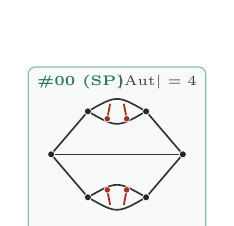
\begin{tikzpicture}[scale=0.88, baseline={(0,0)}]
  \draw[rounded corners=2.5pt, draw=PineGreen!80!black!45, fill=PineGreen!80!black!3, line width=0.45pt] (-1.28,-1.18) rectangle (1.28,1.26);
  \node[anchor=north west, font=\tiny\bfseries, text=PineGreen!80!black, inner sep=1.5pt] at (-1.22,1.21) {\#00 (SP)};
  \node[anchor=north east, font=\tiny, text=black!75, inner sep=1.5pt] at (1.22,1.21) {$|\mathrm{Aut}|=4$};
  \draw[line width=0.6pt, draw=black!80] (-0.950,0.000) -- (-0.420,0.620);
  \draw[line width=0.6pt, draw=black!80] (-0.950,0.000) -- (0.950,0.000);
  \draw[line width=0.6pt, draw=black!80] (-0.950,0.000) -- (-0.420,-0.620);
  \draw[line width=0.6pt, draw=black!80] (-0.420,0.620) .. controls (0.000,0.860) .. (0.420,0.620);
  \draw[line width=0.6pt, draw=black!80] (-0.420,0.620) .. controls (0.000,0.380) .. (0.420,0.620);
  \draw[line width=0.6pt, draw=black!80] (0.420,0.620) -- (0.950,0.000);
  \draw[line width=0.6pt, draw=black!80] (0.950,0.000) -- (0.420,-0.620);
  \draw[line width=0.6pt, draw=black!80] (0.420,-0.620) .. controls (0.000,-0.860) .. (-0.420,-0.620);
  \draw[line width=0.6pt, draw=black!80] (0.420,-0.620) .. controls (0.000,-0.380) .. (-0.420,-0.620);
  \draw[line width=0.65pt, draw=BrickRed!85!black] (-0.140,0.513) -- (-0.099,0.729);
  \filldraw[fill=BrickRed!85!black, draw=white, line width=0.25pt] (-0.140,0.513) circle (1.35pt);
  \draw[line width=0.65pt, draw=BrickRed!85!black] (0.140,0.513) -- (0.099,0.729);
  \filldraw[fill=BrickRed!85!black, draw=white, line width=0.25pt] (0.140,0.513) circle (1.35pt);
  \draw[line width=0.65pt, draw=BrickRed!85!black] (0.140,-0.513) -- (0.099,-0.729);
  \filldraw[fill=BrickRed!85!black, draw=white, line width=0.25pt] (0.140,-0.513) circle (1.35pt);
  \draw[line width=0.65pt, draw=BrickRed!85!black] (-0.140,-0.513) -- (-0.099,-0.729);
  \filldraw[fill=BrickRed!85!black, draw=white, line width=0.25pt] (-0.140,-0.513) circle (1.35pt);
  \filldraw[fill=black!85, draw=white, line width=0.25pt] (-0.950,0.000) circle (1.45pt);
  \filldraw[fill=black!85, draw=white, line width=0.25pt] (0.950,0.000) circle (1.45pt);
  \filldraw[fill=black!85, draw=white, line width=0.25pt] (-0.420,0.620) circle (1.45pt);
  \filldraw[fill=black!85, draw=white, line width=0.25pt] (0.420,0.620) circle (1.45pt);
  \filldraw[fill=black!85, draw=white, line width=0.25pt] (-0.420,-0.620) circle (1.45pt);
  \filldraw[fill=black!85, draw=white, line width=0.25pt] (0.420,-0.620) circle (1.45pt);
\end{tikzpicture} &
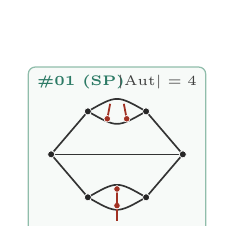
\begin{tikzpicture}[scale=0.88, baseline={(0,0)}]
  \draw[rounded corners=2.5pt, draw=PineGreen!80!black!45, fill=PineGreen!80!black!3, line width=0.45pt] (-1.28,-1.18) rectangle (1.28,1.26);
  \node[anchor=north west, font=\tiny\bfseries, text=PineGreen!80!black, inner sep=1.5pt] at (-1.22,1.21) {\#01 (SP)};
  \node[anchor=north east, font=\tiny, text=black!75, inner sep=1.5pt] at (1.22,1.21) {$|\mathrm{Aut}|=4$};
  \draw[line width=0.6pt, draw=black!80] (-0.950,0.000) -- (-0.420,0.620);
  \draw[line width=0.6pt, draw=black!80] (-0.950,0.000) -- (0.950,0.000);
  \draw[line width=0.6pt, draw=black!80] (-0.950,0.000) -- (-0.420,-0.620);
  \draw[line width=0.6pt, draw=black!80] (-0.420,0.620) .. controls (0.000,0.860) .. (0.420,0.620);
  \draw[line width=0.6pt, draw=black!80] (-0.420,0.620) .. controls (0.000,0.380) .. (0.420,0.620);
  \draw[line width=0.6pt, draw=black!80] (0.420,0.620) -- (0.950,0.000);
  \draw[line width=0.6pt, draw=black!80] (0.950,0.000) -- (0.420,-0.620);
  \draw[line width=0.6pt, draw=black!80] (0.420,-0.620) .. controls (0.000,-0.860) .. (-0.420,-0.620);
  \draw[line width=0.6pt, draw=black!80] (0.420,-0.620) .. controls (0.000,-0.380) .. (-0.420,-0.620);
  \draw[line width=0.65pt, draw=BrickRed!85!black] (-0.140,0.513) -- (-0.099,0.729);
  \filldraw[fill=BrickRed!85!black, draw=white, line width=0.25pt] (-0.140,0.513) circle (1.35pt);
  \draw[line width=0.65pt, draw=BrickRed!85!black] (0.140,0.513) -- (0.099,0.729);
  \filldraw[fill=BrickRed!85!black, draw=white, line width=0.25pt] (0.140,0.513) circle (1.35pt);
  \draw[line width=0.65pt, draw=BrickRed!85!black] (0.000,-0.740) -- (0.000,-0.960);
  \filldraw[fill=BrickRed!85!black, draw=white, line width=0.25pt] (0.000,-0.740) circle (1.35pt);
  \draw[line width=0.65pt, draw=BrickRed!85!black] (0.000,-0.500) -- (0.000,-0.720);
  \filldraw[fill=BrickRed!85!black, draw=white, line width=0.25pt] (0.000,-0.500) circle (1.35pt);
  \filldraw[fill=black!85, draw=white, line width=0.25pt] (-0.950,0.000) circle (1.45pt);
  \filldraw[fill=black!85, draw=white, line width=0.25pt] (0.950,0.000) circle (1.45pt);
  \filldraw[fill=black!85, draw=white, line width=0.25pt] (-0.420,0.620) circle (1.45pt);
  \filldraw[fill=black!85, draw=white, line width=0.25pt] (0.420,0.620) circle (1.45pt);
  \filldraw[fill=black!85, draw=white, line width=0.25pt] (-0.420,-0.620) circle (1.45pt);
  \filldraw[fill=black!85, draw=white, line width=0.25pt] (0.420,-0.620) circle (1.45pt);
\end{tikzpicture} &
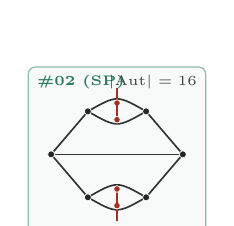
\begin{tikzpicture}[scale=0.88, baseline={(0,0)}]
  \draw[rounded corners=2.5pt, draw=PineGreen!80!black!45, fill=PineGreen!80!black!3, line width=0.45pt] (-1.28,-1.18) rectangle (1.28,1.26);
  \node[anchor=north west, font=\tiny\bfseries, text=PineGreen!80!black, inner sep=1.5pt] at (-1.22,1.21) {\#02 (SP)};
  \node[anchor=north east, font=\tiny, text=black!75, inner sep=1.5pt] at (1.22,1.21) {$|\mathrm{Aut}|=16$};
  \draw[line width=0.6pt, draw=black!80] (-0.950,0.000) -- (-0.420,0.620);
  \draw[line width=0.6pt, draw=black!80] (-0.950,0.000) -- (0.950,0.000);
  \draw[line width=0.6pt, draw=black!80] (-0.950,0.000) -- (-0.420,-0.620);
  \draw[line width=0.6pt, draw=black!80] (-0.420,0.620) .. controls (0.000,0.860) .. (0.420,0.620);
  \draw[line width=0.6pt, draw=black!80] (-0.420,0.620) .. controls (0.000,0.380) .. (0.420,0.620);
  \draw[line width=0.6pt, draw=black!80] (0.420,0.620) -- (0.950,0.000);
  \draw[line width=0.6pt, draw=black!80] (0.950,0.000) -- (0.420,-0.620);
  \draw[line width=0.6pt, draw=black!80] (0.420,-0.620) .. controls (0.000,-0.860) .. (-0.420,-0.620);
  \draw[line width=0.6pt, draw=black!80] (0.420,-0.620) .. controls (0.000,-0.380) .. (-0.420,-0.620);
  \draw[line width=0.65pt, draw=BrickRed!85!black] (0.000,0.740) -- (0.000,0.960);
  \filldraw[fill=BrickRed!85!black, draw=white, line width=0.25pt] (0.000,0.740) circle (1.35pt);
  \draw[line width=0.65pt, draw=BrickRed!85!black] (0.000,0.500) -- (0.000,0.720);
  \filldraw[fill=BrickRed!85!black, draw=white, line width=0.25pt] (0.000,0.500) circle (1.35pt);
  \draw[line width=0.65pt, draw=BrickRed!85!black] (0.000,-0.740) -- (0.000,-0.960);
  \filldraw[fill=BrickRed!85!black, draw=white, line width=0.25pt] (0.000,-0.740) circle (1.35pt);
  \draw[line width=0.65pt, draw=BrickRed!85!black] (0.000,-0.500) -- (0.000,-0.720);
  \filldraw[fill=BrickRed!85!black, draw=white, line width=0.25pt] (0.000,-0.500) circle (1.35pt);
  \filldraw[fill=black!85, draw=white, line width=0.25pt] (-0.950,0.000) circle (1.45pt);
  \filldraw[fill=black!85, draw=white, line width=0.25pt] (0.950,0.000) circle (1.45pt);
  \filldraw[fill=black!85, draw=white, line width=0.25pt] (-0.420,0.620) circle (1.45pt);
  \filldraw[fill=black!85, draw=white, line width=0.25pt] (0.420,0.620) circle (1.45pt);
  \filldraw[fill=black!85, draw=white, line width=0.25pt] (-0.420,-0.620) circle (1.45pt);
  \filldraw[fill=black!85, draw=white, line width=0.25pt] (0.420,-0.620) circle (1.45pt);
\end{tikzpicture} &
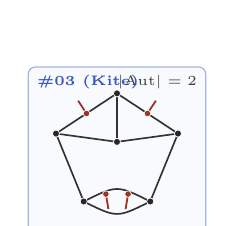
\begin{tikzpicture}[scale=0.88, baseline={(0,0)}]
  \draw[rounded corners=2.5pt, draw=RoyalBlue!85!black!45, fill=RoyalBlue!85!black!3, line width=0.45pt] (-1.28,-1.18) rectangle (1.28,1.26);
  \node[anchor=north west, font=\tiny\bfseries, text=RoyalBlue!85!black, inner sep=1.5pt] at (-1.22,1.21) {\#03 (Kite)};
  \node[anchor=north east, font=\tiny, text=black!75, inner sep=1.5pt] at (1.22,1.21) {$|\mathrm{Aut}|=2$};
  \draw[line width=0.6pt, draw=black!80] (-0.880,0.300) -- (0.000,0.880);
  \draw[line width=0.6pt, draw=black!80] (-0.880,0.300) -- (-0.480,-0.680);
  \draw[line width=0.6pt, draw=black!80] (-0.880,0.300) -- (0.000,0.180);
  \draw[line width=0.6pt, draw=black!80] (0.000,0.880) -- (0.880,0.300);
  \draw[line width=0.6pt, draw=black!80] (0.000,0.880) -- (0.000,0.180);
  \draw[line width=0.6pt, draw=black!80] (0.880,0.300) -- (0.480,-0.680);
  \draw[line width=0.6pt, draw=black!80] (0.880,0.300) -- (0.000,0.180);
  \draw[line width=0.6pt, draw=black!80] (0.480,-0.680) .. controls (0.000,-0.920) .. (-0.480,-0.680);
  \draw[line width=0.6pt, draw=black!80] (0.480,-0.680) .. controls (0.000,-0.440) .. (-0.480,-0.680);
  \draw[line width=0.65pt, draw=BrickRed!85!black] (-0.440,0.590) -- (-0.561,0.774);
  \filldraw[fill=BrickRed!85!black, draw=white, line width=0.25pt] (-0.440,0.590) circle (1.35pt);
  \draw[line width=0.65pt, draw=BrickRed!85!black] (0.440,0.590) -- (0.561,0.774);
  \filldraw[fill=BrickRed!85!black, draw=white, line width=0.25pt] (0.440,0.590) circle (1.35pt);
  \draw[line width=0.65pt, draw=BrickRed!85!black] (0.160,-0.573) -- (0.124,-0.790);
  \filldraw[fill=BrickRed!85!black, draw=white, line width=0.25pt] (0.160,-0.573) circle (1.35pt);
  \draw[line width=0.65pt, draw=BrickRed!85!black] (-0.160,-0.573) -- (-0.124,-0.790);
  \filldraw[fill=BrickRed!85!black, draw=white, line width=0.25pt] (-0.160,-0.573) circle (1.35pt);
  \filldraw[fill=black!85, draw=white, line width=0.25pt] (0.000,0.180) circle (1.45pt);
  \filldraw[fill=black!85, draw=white, line width=0.25pt] (0.000,0.880) circle (1.45pt);
  \filldraw[fill=black!85, draw=white, line width=0.25pt] (-0.880,0.300) circle (1.45pt);
  \filldraw[fill=black!85, draw=white, line width=0.25pt] (0.880,0.300) circle (1.45pt);
  \filldraw[fill=black!85, draw=white, line width=0.25pt] (-0.480,-0.680) circle (1.45pt);
  \filldraw[fill=black!85, draw=white, line width=0.25pt] (0.480,-0.680) circle (1.45pt);
\end{tikzpicture} &
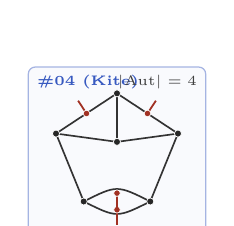
\begin{tikzpicture}[scale=0.88, baseline={(0,0)}]
  \draw[rounded corners=2.5pt, draw=RoyalBlue!85!black!45, fill=RoyalBlue!85!black!3, line width=0.45pt] (-1.28,-1.18) rectangle (1.28,1.26);
  \node[anchor=north west, font=\tiny\bfseries, text=RoyalBlue!85!black, inner sep=1.5pt] at (-1.22,1.21) {\#04 (Kite)};
  \node[anchor=north east, font=\tiny, text=black!75, inner sep=1.5pt] at (1.22,1.21) {$|\mathrm{Aut}|=4$};
  \draw[line width=0.6pt, draw=black!80] (-0.880,0.300) -- (0.000,0.880);
  \draw[line width=0.6pt, draw=black!80] (-0.880,0.300) -- (-0.480,-0.680);
  \draw[line width=0.6pt, draw=black!80] (-0.880,0.300) -- (0.000,0.180);
  \draw[line width=0.6pt, draw=black!80] (0.000,0.880) -- (0.880,0.300);
  \draw[line width=0.6pt, draw=black!80] (0.000,0.880) -- (0.000,0.180);
  \draw[line width=0.6pt, draw=black!80] (0.880,0.300) -- (0.480,-0.680);
  \draw[line width=0.6pt, draw=black!80] (0.880,0.300) -- (0.000,0.180);
  \draw[line width=0.6pt, draw=black!80] (0.480,-0.680) .. controls (0.000,-0.920) .. (-0.480,-0.680);
  \draw[line width=0.6pt, draw=black!80] (0.480,-0.680) .. controls (0.000,-0.440) .. (-0.480,-0.680);
  \draw[line width=0.65pt, draw=BrickRed!85!black] (-0.440,0.590) -- (-0.561,0.774);
  \filldraw[fill=BrickRed!85!black, draw=white, line width=0.25pt] (-0.440,0.590) circle (1.35pt);
  \draw[line width=0.65pt, draw=BrickRed!85!black] (0.440,0.590) -- (0.561,0.774);
  \filldraw[fill=BrickRed!85!black, draw=white, line width=0.25pt] (0.440,0.590) circle (1.35pt);
  \draw[line width=0.65pt, draw=BrickRed!85!black] (0.000,-0.800) -- (0.000,-1.020);
  \filldraw[fill=BrickRed!85!black, draw=white, line width=0.25pt] (0.000,-0.800) circle (1.35pt);
  \draw[line width=0.65pt, draw=BrickRed!85!black] (0.000,-0.560) -- (0.000,-0.780);
  \filldraw[fill=BrickRed!85!black, draw=white, line width=0.25pt] (0.000,-0.560) circle (1.35pt);
  \filldraw[fill=black!85, draw=white, line width=0.25pt] (0.000,0.180) circle (1.45pt);
  \filldraw[fill=black!85, draw=white, line width=0.25pt] (0.000,0.880) circle (1.45pt);
  \filldraw[fill=black!85, draw=white, line width=0.25pt] (-0.880,0.300) circle (1.45pt);
  \filldraw[fill=black!85, draw=white, line width=0.25pt] (0.880,0.300) circle (1.45pt);
  \filldraw[fill=black!85, draw=white, line width=0.25pt] (-0.480,-0.680) circle (1.45pt);
  \filldraw[fill=black!85, draw=white, line width=0.25pt] (0.480,-0.680) circle (1.45pt);
\end{tikzpicture} \\[2pt]
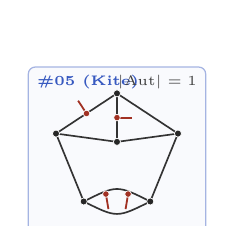
\begin{tikzpicture}[scale=0.88, baseline={(0,0)}]
  \draw[rounded corners=2.5pt, draw=RoyalBlue!85!black!45, fill=RoyalBlue!85!black!3, line width=0.45pt] (-1.28,-1.18) rectangle (1.28,1.26);
  \node[anchor=north west, font=\tiny\bfseries, text=RoyalBlue!85!black, inner sep=1.5pt] at (-1.22,1.21) {\#05 (Kite)};
  \node[anchor=north east, font=\tiny, text=black!75, inner sep=1.5pt] at (1.22,1.21) {$|\mathrm{Aut}|=1$};
  \draw[line width=0.6pt, draw=black!80] (-0.880,0.300) -- (0.000,0.880);
  \draw[line width=0.6pt, draw=black!80] (-0.880,0.300) -- (-0.480,-0.680);
  \draw[line width=0.6pt, draw=black!80] (-0.880,0.300) -- (0.000,0.180);
  \draw[line width=0.6pt, draw=black!80] (0.000,0.880) -- (0.880,0.300);
  \draw[line width=0.6pt, draw=black!80] (0.000,0.880) -- (0.000,0.180);
  \draw[line width=0.6pt, draw=black!80] (0.880,0.300) -- (0.480,-0.680);
  \draw[line width=0.6pt, draw=black!80] (0.880,0.300) -- (0.000,0.180);
  \draw[line width=0.6pt, draw=black!80] (0.480,-0.680) .. controls (0.000,-0.920) .. (-0.480,-0.680);
  \draw[line width=0.6pt, draw=black!80] (0.480,-0.680) .. controls (0.000,-0.440) .. (-0.480,-0.680);
  \draw[line width=0.65pt, draw=BrickRed!85!black] (-0.440,0.590) -- (-0.561,0.774);
  \filldraw[fill=BrickRed!85!black, draw=white, line width=0.25pt] (-0.440,0.590) circle (1.35pt);
  \draw[line width=0.65pt, draw=BrickRed!85!black] (0.000,0.530) -- (0.220,0.530);
  \filldraw[fill=BrickRed!85!black, draw=white, line width=0.25pt] (0.000,0.530) circle (1.35pt);
  \draw[line width=0.65pt, draw=BrickRed!85!black] (0.160,-0.573) -- (0.124,-0.790);
  \filldraw[fill=BrickRed!85!black, draw=white, line width=0.25pt] (0.160,-0.573) circle (1.35pt);
  \draw[line width=0.65pt, draw=BrickRed!85!black] (-0.160,-0.573) -- (-0.124,-0.790);
  \filldraw[fill=BrickRed!85!black, draw=white, line width=0.25pt] (-0.160,-0.573) circle (1.35pt);
  \filldraw[fill=black!85, draw=white, line width=0.25pt] (0.000,0.180) circle (1.45pt);
  \filldraw[fill=black!85, draw=white, line width=0.25pt] (0.000,0.880) circle (1.45pt);
  \filldraw[fill=black!85, draw=white, line width=0.25pt] (-0.880,0.300) circle (1.45pt);
  \filldraw[fill=black!85, draw=white, line width=0.25pt] (0.880,0.300) circle (1.45pt);
  \filldraw[fill=black!85, draw=white, line width=0.25pt] (-0.480,-0.680) circle (1.45pt);
  \filldraw[fill=black!85, draw=white, line width=0.25pt] (0.480,-0.680) circle (1.45pt);
\end{tikzpicture} &
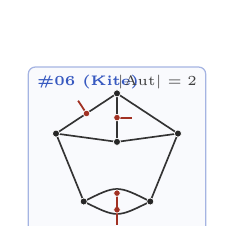
\begin{tikzpicture}[scale=0.88, baseline={(0,0)}]
  \draw[rounded corners=2.5pt, draw=RoyalBlue!85!black!45, fill=RoyalBlue!85!black!3, line width=0.45pt] (-1.28,-1.18) rectangle (1.28,1.26);
  \node[anchor=north west, font=\tiny\bfseries, text=RoyalBlue!85!black, inner sep=1.5pt] at (-1.22,1.21) {\#06 (Kite)};
  \node[anchor=north east, font=\tiny, text=black!75, inner sep=1.5pt] at (1.22,1.21) {$|\mathrm{Aut}|=2$};
  \draw[line width=0.6pt, draw=black!80] (-0.880,0.300) -- (0.000,0.880);
  \draw[line width=0.6pt, draw=black!80] (-0.880,0.300) -- (-0.480,-0.680);
  \draw[line width=0.6pt, draw=black!80] (-0.880,0.300) -- (0.000,0.180);
  \draw[line width=0.6pt, draw=black!80] (0.000,0.880) -- (0.880,0.300);
  \draw[line width=0.6pt, draw=black!80] (0.000,0.880) -- (0.000,0.180);
  \draw[line width=0.6pt, draw=black!80] (0.880,0.300) -- (0.480,-0.680);
  \draw[line width=0.6pt, draw=black!80] (0.880,0.300) -- (0.000,0.180);
  \draw[line width=0.6pt, draw=black!80] (0.480,-0.680) .. controls (0.000,-0.920) .. (-0.480,-0.680);
  \draw[line width=0.6pt, draw=black!80] (0.480,-0.680) .. controls (0.000,-0.440) .. (-0.480,-0.680);
  \draw[line width=0.65pt, draw=BrickRed!85!black] (-0.440,0.590) -- (-0.561,0.774);
  \filldraw[fill=BrickRed!85!black, draw=white, line width=0.25pt] (-0.440,0.590) circle (1.35pt);
  \draw[line width=0.65pt, draw=BrickRed!85!black] (0.000,0.530) -- (0.220,0.530);
  \filldraw[fill=BrickRed!85!black, draw=white, line width=0.25pt] (0.000,0.530) circle (1.35pt);
  \draw[line width=0.65pt, draw=BrickRed!85!black] (0.000,-0.800) -- (0.000,-1.020);
  \filldraw[fill=BrickRed!85!black, draw=white, line width=0.25pt] (0.000,-0.800) circle (1.35pt);
  \draw[line width=0.65pt, draw=BrickRed!85!black] (0.000,-0.560) -- (0.000,-0.780);
  \filldraw[fill=BrickRed!85!black, draw=white, line width=0.25pt] (0.000,-0.560) circle (1.35pt);
  \filldraw[fill=black!85, draw=white, line width=0.25pt] (0.000,0.180) circle (1.45pt);
  \filldraw[fill=black!85, draw=white, line width=0.25pt] (0.000,0.880) circle (1.45pt);
  \filldraw[fill=black!85, draw=white, line width=0.25pt] (-0.880,0.300) circle (1.45pt);
  \filldraw[fill=black!85, draw=white, line width=0.25pt] (0.880,0.300) circle (1.45pt);
  \filldraw[fill=black!85, draw=white, line width=0.25pt] (-0.480,-0.680) circle (1.45pt);
  \filldraw[fill=black!85, draw=white, line width=0.25pt] (0.480,-0.680) circle (1.45pt);
\end{tikzpicture} &
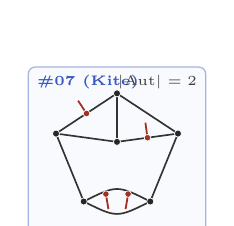
\begin{tikzpicture}[scale=0.88, baseline={(0,0)}]
  \draw[rounded corners=2.5pt, draw=RoyalBlue!85!black!45, fill=RoyalBlue!85!black!3, line width=0.45pt] (-1.28,-1.18) rectangle (1.28,1.26);
  \node[anchor=north west, font=\tiny\bfseries, text=RoyalBlue!85!black, inner sep=1.5pt] at (-1.22,1.21) {\#07 (Kite)};
  \node[anchor=north east, font=\tiny, text=black!75, inner sep=1.5pt] at (1.22,1.21) {$|\mathrm{Aut}|=2$};
  \draw[line width=0.6pt, draw=black!80] (-0.880,0.300) -- (0.000,0.880);
  \draw[line width=0.6pt, draw=black!80] (-0.880,0.300) -- (-0.480,-0.680);
  \draw[line width=0.6pt, draw=black!80] (-0.880,0.300) -- (0.000,0.180);
  \draw[line width=0.6pt, draw=black!80] (0.000,0.880) -- (0.880,0.300);
  \draw[line width=0.6pt, draw=black!80] (0.000,0.880) -- (0.000,0.180);
  \draw[line width=0.6pt, draw=black!80] (0.880,0.300) -- (0.480,-0.680);
  \draw[line width=0.6pt, draw=black!80] (0.880,0.300) -- (0.000,0.180);
  \draw[line width=0.6pt, draw=black!80] (0.480,-0.680) .. controls (0.000,-0.920) .. (-0.480,-0.680);
  \draw[line width=0.6pt, draw=black!80] (0.480,-0.680) .. controls (0.000,-0.440) .. (-0.480,-0.680);
  \draw[line width=0.65pt, draw=BrickRed!85!black] (-0.440,0.590) -- (-0.561,0.774);
  \filldraw[fill=BrickRed!85!black, draw=white, line width=0.25pt] (-0.440,0.590) circle (1.35pt);
  \draw[line width=0.65pt, draw=BrickRed!85!black] (0.440,0.240) -- (0.410,0.458);
  \filldraw[fill=BrickRed!85!black, draw=white, line width=0.25pt] (0.440,0.240) circle (1.35pt);
  \draw[line width=0.65pt, draw=BrickRed!85!black] (0.160,-0.573) -- (0.124,-0.790);
  \filldraw[fill=BrickRed!85!black, draw=white, line width=0.25pt] (0.160,-0.573) circle (1.35pt);
  \draw[line width=0.65pt, draw=BrickRed!85!black] (-0.160,-0.573) -- (-0.124,-0.790);
  \filldraw[fill=BrickRed!85!black, draw=white, line width=0.25pt] (-0.160,-0.573) circle (1.35pt);
  \filldraw[fill=black!85, draw=white, line width=0.25pt] (0.000,0.180) circle (1.45pt);
  \filldraw[fill=black!85, draw=white, line width=0.25pt] (0.000,0.880) circle (1.45pt);
  \filldraw[fill=black!85, draw=white, line width=0.25pt] (-0.880,0.300) circle (1.45pt);
  \filldraw[fill=black!85, draw=white, line width=0.25pt] (0.880,0.300) circle (1.45pt);
  \filldraw[fill=black!85, draw=white, line width=0.25pt] (-0.480,-0.680) circle (1.45pt);
  \filldraw[fill=black!85, draw=white, line width=0.25pt] (0.480,-0.680) circle (1.45pt);
\end{tikzpicture} &
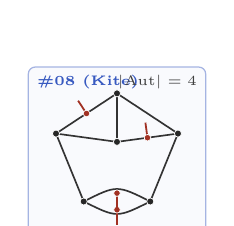
\begin{tikzpicture}[scale=0.88, baseline={(0,0)}]
  \draw[rounded corners=2.5pt, draw=RoyalBlue!85!black!45, fill=RoyalBlue!85!black!3, line width=0.45pt] (-1.28,-1.18) rectangle (1.28,1.26);
  \node[anchor=north west, font=\tiny\bfseries, text=RoyalBlue!85!black, inner sep=1.5pt] at (-1.22,1.21) {\#08 (Kite)};
  \node[anchor=north east, font=\tiny, text=black!75, inner sep=1.5pt] at (1.22,1.21) {$|\mathrm{Aut}|=4$};
  \draw[line width=0.6pt, draw=black!80] (-0.880,0.300) -- (0.000,0.880);
  \draw[line width=0.6pt, draw=black!80] (-0.880,0.300) -- (-0.480,-0.680);
  \draw[line width=0.6pt, draw=black!80] (-0.880,0.300) -- (0.000,0.180);
  \draw[line width=0.6pt, draw=black!80] (0.000,0.880) -- (0.880,0.300);
  \draw[line width=0.6pt, draw=black!80] (0.000,0.880) -- (0.000,0.180);
  \draw[line width=0.6pt, draw=black!80] (0.880,0.300) -- (0.480,-0.680);
  \draw[line width=0.6pt, draw=black!80] (0.880,0.300) -- (0.000,0.180);
  \draw[line width=0.6pt, draw=black!80] (0.480,-0.680) .. controls (0.000,-0.920) .. (-0.480,-0.680);
  \draw[line width=0.6pt, draw=black!80] (0.480,-0.680) .. controls (0.000,-0.440) .. (-0.480,-0.680);
  \draw[line width=0.65pt, draw=BrickRed!85!black] (-0.440,0.590) -- (-0.561,0.774);
  \filldraw[fill=BrickRed!85!black, draw=white, line width=0.25pt] (-0.440,0.590) circle (1.35pt);
  \draw[line width=0.65pt, draw=BrickRed!85!black] (0.440,0.240) -- (0.410,0.458);
  \filldraw[fill=BrickRed!85!black, draw=white, line width=0.25pt] (0.440,0.240) circle (1.35pt);
  \draw[line width=0.65pt, draw=BrickRed!85!black] (0.000,-0.800) -- (0.000,-1.020);
  \filldraw[fill=BrickRed!85!black, draw=white, line width=0.25pt] (0.000,-0.800) circle (1.35pt);
  \draw[line width=0.65pt, draw=BrickRed!85!black] (0.000,-0.560) -- (0.000,-0.780);
  \filldraw[fill=BrickRed!85!black, draw=white, line width=0.25pt] (0.000,-0.560) circle (1.35pt);
  \filldraw[fill=black!85, draw=white, line width=0.25pt] (0.000,0.180) circle (1.45pt);
  \filldraw[fill=black!85, draw=white, line width=0.25pt] (0.000,0.880) circle (1.45pt);
  \filldraw[fill=black!85, draw=white, line width=0.25pt] (-0.880,0.300) circle (1.45pt);
  \filldraw[fill=black!85, draw=white, line width=0.25pt] (0.880,0.300) circle (1.45pt);
  \filldraw[fill=black!85, draw=white, line width=0.25pt] (-0.480,-0.680) circle (1.45pt);
  \filldraw[fill=black!85, draw=white, line width=0.25pt] (0.480,-0.680) circle (1.45pt);
\end{tikzpicture} &
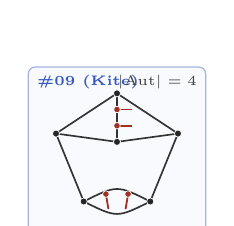
\begin{tikzpicture}[scale=0.88, baseline={(0,0)}]
  \draw[rounded corners=2.5pt, draw=RoyalBlue!85!black!45, fill=RoyalBlue!85!black!3, line width=0.45pt] (-1.28,-1.18) rectangle (1.28,1.26);
  \node[anchor=north west, font=\tiny\bfseries, text=RoyalBlue!85!black, inner sep=1.5pt] at (-1.22,1.21) {\#09 (Kite)};
  \node[anchor=north east, font=\tiny, text=black!75, inner sep=1.5pt] at (1.22,1.21) {$|\mathrm{Aut}|=4$};
  \draw[line width=0.6pt, draw=black!80] (-0.880,0.300) -- (0.000,0.880);
  \draw[line width=0.6pt, draw=black!80] (-0.880,0.300) -- (-0.480,-0.680);
  \draw[line width=0.6pt, draw=black!80] (-0.880,0.300) -- (0.000,0.180);
  \draw[line width=0.6pt, draw=black!80] (0.000,0.880) -- (0.880,0.300);
  \draw[line width=0.6pt, draw=black!80] (0.000,0.880) -- (0.000,0.180);
  \draw[line width=0.6pt, draw=black!80] (0.880,0.300) -- (0.480,-0.680);
  \draw[line width=0.6pt, draw=black!80] (0.880,0.300) -- (0.000,0.180);
  \draw[line width=0.6pt, draw=black!80] (0.480,-0.680) .. controls (0.000,-0.920) .. (-0.480,-0.680);
  \draw[line width=0.6pt, draw=black!80] (0.480,-0.680) .. controls (0.000,-0.440) .. (-0.480,-0.680);
  \draw[line width=0.65pt, draw=BrickRed!85!black] (0.000,0.647) -- (0.220,0.647);
  \filldraw[fill=BrickRed!85!black, draw=white, line width=0.25pt] (0.000,0.647) circle (1.35pt);
  \draw[line width=0.65pt, draw=BrickRed!85!black] (0.000,0.413) -- (0.220,0.413);
  \filldraw[fill=BrickRed!85!black, draw=white, line width=0.25pt] (0.000,0.413) circle (1.35pt);
  \draw[line width=0.65pt, draw=BrickRed!85!black] (0.160,-0.573) -- (0.124,-0.790);
  \filldraw[fill=BrickRed!85!black, draw=white, line width=0.25pt] (0.160,-0.573) circle (1.35pt);
  \draw[line width=0.65pt, draw=BrickRed!85!black] (-0.160,-0.573) -- (-0.124,-0.790);
  \filldraw[fill=BrickRed!85!black, draw=white, line width=0.25pt] (-0.160,-0.573) circle (1.35pt);
  \filldraw[fill=black!85, draw=white, line width=0.25pt] (0.000,0.180) circle (1.45pt);
  \filldraw[fill=black!85, draw=white, line width=0.25pt] (0.000,0.880) circle (1.45pt);
  \filldraw[fill=black!85, draw=white, line width=0.25pt] (-0.880,0.300) circle (1.45pt);
  \filldraw[fill=black!85, draw=white, line width=0.25pt] (0.880,0.300) circle (1.45pt);
  \filldraw[fill=black!85, draw=white, line width=0.25pt] (-0.480,-0.680) circle (1.45pt);
  \filldraw[fill=black!85, draw=white, line width=0.25pt] (0.480,-0.680) circle (1.45pt);
\end{tikzpicture} \\[2pt]
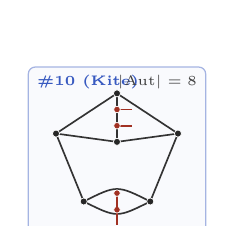
\begin{tikzpicture}[scale=0.88, baseline={(0,0)}]
  \draw[rounded corners=2.5pt, draw=RoyalBlue!85!black!45, fill=RoyalBlue!85!black!3, line width=0.45pt] (-1.28,-1.18) rectangle (1.28,1.26);
  \node[anchor=north west, font=\tiny\bfseries, text=RoyalBlue!85!black, inner sep=1.5pt] at (-1.22,1.21) {\#10 (Kite)};
  \node[anchor=north east, font=\tiny, text=black!75, inner sep=1.5pt] at (1.22,1.21) {$|\mathrm{Aut}|=8$};
  \draw[line width=0.6pt, draw=black!80] (-0.880,0.300) -- (0.000,0.880);
  \draw[line width=0.6pt, draw=black!80] (-0.880,0.300) -- (-0.480,-0.680);
  \draw[line width=0.6pt, draw=black!80] (-0.880,0.300) -- (0.000,0.180);
  \draw[line width=0.6pt, draw=black!80] (0.000,0.880) -- (0.880,0.300);
  \draw[line width=0.6pt, draw=black!80] (0.000,0.880) -- (0.000,0.180);
  \draw[line width=0.6pt, draw=black!80] (0.880,0.300) -- (0.480,-0.680);
  \draw[line width=0.6pt, draw=black!80] (0.880,0.300) -- (0.000,0.180);
  \draw[line width=0.6pt, draw=black!80] (0.480,-0.680) .. controls (0.000,-0.920) .. (-0.480,-0.680);
  \draw[line width=0.6pt, draw=black!80] (0.480,-0.680) .. controls (0.000,-0.440) .. (-0.480,-0.680);
  \draw[line width=0.65pt, draw=BrickRed!85!black] (0.000,0.647) -- (0.220,0.647);
  \filldraw[fill=BrickRed!85!black, draw=white, line width=0.25pt] (0.000,0.647) circle (1.35pt);
  \draw[line width=0.65pt, draw=BrickRed!85!black] (0.000,0.413) -- (0.220,0.413);
  \filldraw[fill=BrickRed!85!black, draw=white, line width=0.25pt] (0.000,0.413) circle (1.35pt);
  \draw[line width=0.65pt, draw=BrickRed!85!black] (0.000,-0.800) -- (0.000,-1.020);
  \filldraw[fill=BrickRed!85!black, draw=white, line width=0.25pt] (0.000,-0.800) circle (1.35pt);
  \draw[line width=0.65pt, draw=BrickRed!85!black] (0.000,-0.560) -- (0.000,-0.780);
  \filldraw[fill=BrickRed!85!black, draw=white, line width=0.25pt] (0.000,-0.560) circle (1.35pt);
  \filldraw[fill=black!85, draw=white, line width=0.25pt] (0.000,0.180) circle (1.45pt);
  \filldraw[fill=black!85, draw=white, line width=0.25pt] (0.000,0.880) circle (1.45pt);
  \filldraw[fill=black!85, draw=white, line width=0.25pt] (-0.880,0.300) circle (1.45pt);
  \filldraw[fill=black!85, draw=white, line width=0.25pt] (0.880,0.300) circle (1.45pt);
  \filldraw[fill=black!85, draw=white, line width=0.25pt] (-0.480,-0.680) circle (1.45pt);
  \filldraw[fill=black!85, draw=white, line width=0.25pt] (0.480,-0.680) circle (1.45pt);
\end{tikzpicture} &
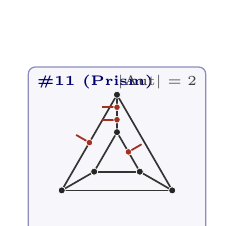
\begin{tikzpicture}[scale=0.88, baseline={(0,0)}]
  \draw[rounded corners=2.5pt, draw=NavyBlue!85!black!45, fill=NavyBlue!85!black!3, line width=0.45pt] (-1.28,-1.18) rectangle (1.28,1.26);
  \node[anchor=north west, font=\tiny\bfseries, text=NavyBlue!85!black, inner sep=1.5pt] at (-1.22,1.21) {\#11 (Prism)};
  \node[anchor=north east, font=\tiny, text=black!75, inner sep=1.5pt] at (1.22,1.21) {$|\mathrm{Aut}|=2$};
  \draw[line width=0.6pt, draw=black!80] (0.000,0.320) -- (0.000,0.860);
  \draw[line width=0.6pt, draw=black!80] (0.000,0.320) -- (0.329,-0.250);
  \draw[line width=0.6pt, draw=black!80] (0.000,0.320) -- (-0.329,-0.250);
  \draw[line width=0.6pt, draw=black!80] (0.000,0.860) -- (-0.797,-0.520);
  \draw[line width=0.6pt, draw=black!80] (0.000,0.860) -- (0.797,-0.520);
  \draw[line width=0.6pt, draw=black!80] (0.329,-0.250) -- (-0.329,-0.250);
  \draw[line width=0.6pt, draw=black!80] (0.329,-0.250) -- (0.797,-0.520);
  \draw[line width=0.6pt, draw=black!80] (-0.329,-0.250) -- (-0.797,-0.520);
  \draw[line width=0.6pt, draw=black!80] (-0.797,-0.520) -- (0.797,-0.520);
  \draw[line width=0.65pt, draw=BrickRed!85!black] (0.000,0.500) -- (-0.220,0.500);
  \filldraw[fill=BrickRed!85!black, draw=white, line width=0.25pt] (0.000,0.500) circle (1.35pt);
  \draw[line width=0.65pt, draw=BrickRed!85!black] (0.000,0.680) -- (-0.220,0.680);
  \filldraw[fill=BrickRed!85!black, draw=white, line width=0.25pt] (0.000,0.680) circle (1.35pt);
  \draw[line width=0.65pt, draw=BrickRed!85!black] (0.165,0.035) -- (0.355,0.145);
  \filldraw[fill=BrickRed!85!black, draw=white, line width=0.25pt] (0.165,0.035) circle (1.35pt);
  \draw[line width=0.65pt, draw=BrickRed!85!black] (-0.398,0.170) -- (-0.589,0.280);
  \filldraw[fill=BrickRed!85!black, draw=white, line width=0.25pt] (-0.398,0.170) circle (1.35pt);
  \filldraw[fill=black!85, draw=white, line width=0.25pt] (0.000,0.320) circle (1.45pt);
  \filldraw[fill=black!85, draw=white, line width=0.25pt] (-0.329,-0.250) circle (1.45pt);
  \filldraw[fill=black!85, draw=white, line width=0.25pt] (0.329,-0.250) circle (1.45pt);
  \filldraw[fill=black!85, draw=white, line width=0.25pt] (0.000,0.860) circle (1.45pt);
  \filldraw[fill=black!85, draw=white, line width=0.25pt] (-0.797,-0.520) circle (1.45pt);
  \filldraw[fill=black!85, draw=white, line width=0.25pt] (0.797,-0.520) circle (1.45pt);
\end{tikzpicture} &
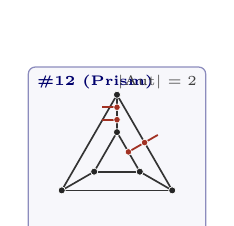
\begin{tikzpicture}[scale=0.88, baseline={(0,0)}]
  \draw[rounded corners=2.5pt, draw=NavyBlue!85!black!45, fill=NavyBlue!85!black!3, line width=0.45pt] (-1.28,-1.18) rectangle (1.28,1.26);
  \node[anchor=north west, font=\tiny\bfseries, text=NavyBlue!85!black, inner sep=1.5pt] at (-1.22,1.21) {\#12 (Prism)};
  \node[anchor=north east, font=\tiny, text=black!75, inner sep=1.5pt] at (1.22,1.21) {$|\mathrm{Aut}|=2$};
  \draw[line width=0.6pt, draw=black!80] (0.000,0.320) -- (0.000,0.860);
  \draw[line width=0.6pt, draw=black!80] (0.000,0.320) -- (0.329,-0.250);
  \draw[line width=0.6pt, draw=black!80] (0.000,0.320) -- (-0.329,-0.250);
  \draw[line width=0.6pt, draw=black!80] (0.000,0.860) -- (-0.797,-0.520);
  \draw[line width=0.6pt, draw=black!80] (0.000,0.860) -- (0.797,-0.520);
  \draw[line width=0.6pt, draw=black!80] (0.329,-0.250) -- (-0.329,-0.250);
  \draw[line width=0.6pt, draw=black!80] (0.329,-0.250) -- (0.797,-0.520);
  \draw[line width=0.6pt, draw=black!80] (-0.329,-0.250) -- (-0.797,-0.520);
  \draw[line width=0.6pt, draw=black!80] (-0.797,-0.520) -- (0.797,-0.520);
  \draw[line width=0.65pt, draw=BrickRed!85!black] (0.000,0.500) -- (-0.220,0.500);
  \filldraw[fill=BrickRed!85!black, draw=white, line width=0.25pt] (0.000,0.500) circle (1.35pt);
  \draw[line width=0.65pt, draw=BrickRed!85!black] (0.000,0.680) -- (-0.220,0.680);
  \filldraw[fill=BrickRed!85!black, draw=white, line width=0.25pt] (0.000,0.680) circle (1.35pt);
  \draw[line width=0.65pt, draw=BrickRed!85!black] (0.165,0.035) -- (0.355,0.145);
  \filldraw[fill=BrickRed!85!black, draw=white, line width=0.25pt] (0.165,0.035) circle (1.35pt);
  \draw[line width=0.65pt, draw=BrickRed!85!black] (0.398,0.170) -- (0.589,0.280);
  \filldraw[fill=BrickRed!85!black, draw=white, line width=0.25pt] (0.398,0.170) circle (1.35pt);
  \filldraw[fill=black!85, draw=white, line width=0.25pt] (0.000,0.320) circle (1.45pt);
  \filldraw[fill=black!85, draw=white, line width=0.25pt] (-0.329,-0.250) circle (1.45pt);
  \filldraw[fill=black!85, draw=white, line width=0.25pt] (0.329,-0.250) circle (1.45pt);
  \filldraw[fill=black!85, draw=white, line width=0.25pt] (0.000,0.860) circle (1.45pt);
  \filldraw[fill=black!85, draw=white, line width=0.25pt] (-0.797,-0.520) circle (1.45pt);
  \filldraw[fill=black!85, draw=white, line width=0.25pt] (0.797,-0.520) circle (1.45pt);
\end{tikzpicture} &
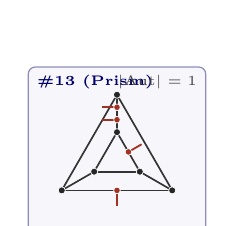
\begin{tikzpicture}[scale=0.88, baseline={(0,0)}]
  \draw[rounded corners=2.5pt, draw=NavyBlue!85!black!45, fill=NavyBlue!85!black!3, line width=0.45pt] (-1.28,-1.18) rectangle (1.28,1.26);
  \node[anchor=north west, font=\tiny\bfseries, text=NavyBlue!85!black, inner sep=1.5pt] at (-1.22,1.21) {\#13 (Prism)};
  \node[anchor=north east, font=\tiny, text=black!75, inner sep=1.5pt] at (1.22,1.21) {$|\mathrm{Aut}|=1$};
  \draw[line width=0.6pt, draw=black!80] (0.000,0.320) -- (0.000,0.860);
  \draw[line width=0.6pt, draw=black!80] (0.000,0.320) -- (0.329,-0.250);
  \draw[line width=0.6pt, draw=black!80] (0.000,0.320) -- (-0.329,-0.250);
  \draw[line width=0.6pt, draw=black!80] (0.000,0.860) -- (-0.797,-0.520);
  \draw[line width=0.6pt, draw=black!80] (0.000,0.860) -- (0.797,-0.520);
  \draw[line width=0.6pt, draw=black!80] (0.329,-0.250) -- (-0.329,-0.250);
  \draw[line width=0.6pt, draw=black!80] (0.329,-0.250) -- (0.797,-0.520);
  \draw[line width=0.6pt, draw=black!80] (-0.329,-0.250) -- (-0.797,-0.520);
  \draw[line width=0.6pt, draw=black!80] (-0.797,-0.520) -- (0.797,-0.520);
  \draw[line width=0.65pt, draw=BrickRed!85!black] (0.000,0.500) -- (-0.220,0.500);
  \filldraw[fill=BrickRed!85!black, draw=white, line width=0.25pt] (0.000,0.500) circle (1.35pt);
  \draw[line width=0.65pt, draw=BrickRed!85!black] (0.000,0.680) -- (-0.220,0.680);
  \filldraw[fill=BrickRed!85!black, draw=white, line width=0.25pt] (0.000,0.680) circle (1.35pt);
  \draw[line width=0.65pt, draw=BrickRed!85!black] (0.165,0.035) -- (0.355,0.145);
  \filldraw[fill=BrickRed!85!black, draw=white, line width=0.25pt] (0.165,0.035) circle (1.35pt);
  \draw[line width=0.65pt, draw=BrickRed!85!black] (-0.000,-0.520) -- (-0.000,-0.740);
  \filldraw[fill=BrickRed!85!black, draw=white, line width=0.25pt] (-0.000,-0.520) circle (1.35pt);
  \filldraw[fill=black!85, draw=white, line width=0.25pt] (0.000,0.320) circle (1.45pt);
  \filldraw[fill=black!85, draw=white, line width=0.25pt] (-0.329,-0.250) circle (1.45pt);
  \filldraw[fill=black!85, draw=white, line width=0.25pt] (0.329,-0.250) circle (1.45pt);
  \filldraw[fill=black!85, draw=white, line width=0.25pt] (0.000,0.860) circle (1.45pt);
  \filldraw[fill=black!85, draw=white, line width=0.25pt] (-0.797,-0.520) circle (1.45pt);
  \filldraw[fill=black!85, draw=white, line width=0.25pt] (0.797,-0.520) circle (1.45pt);
\end{tikzpicture} &
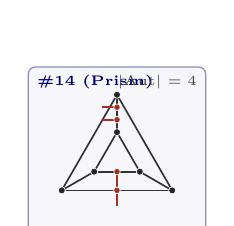
\begin{tikzpicture}[scale=0.88, baseline={(0,0)}]
  \draw[rounded corners=2.5pt, draw=NavyBlue!85!black!45, fill=NavyBlue!85!black!3, line width=0.45pt] (-1.28,-1.18) rectangle (1.28,1.26);
  \node[anchor=north west, font=\tiny\bfseries, text=NavyBlue!85!black, inner sep=1.5pt] at (-1.22,1.21) {\#14 (Prism)};
  \node[anchor=north east, font=\tiny, text=black!75, inner sep=1.5pt] at (1.22,1.21) {$|\mathrm{Aut}|=4$};
  \draw[line width=0.6pt, draw=black!80] (0.000,0.320) -- (0.000,0.860);
  \draw[line width=0.6pt, draw=black!80] (0.000,0.320) -- (0.329,-0.250);
  \draw[line width=0.6pt, draw=black!80] (0.000,0.320) -- (-0.329,-0.250);
  \draw[line width=0.6pt, draw=black!80] (0.000,0.860) -- (-0.797,-0.520);
  \draw[line width=0.6pt, draw=black!80] (0.000,0.860) -- (0.797,-0.520);
  \draw[line width=0.6pt, draw=black!80] (0.329,-0.250) -- (-0.329,-0.250);
  \draw[line width=0.6pt, draw=black!80] (0.329,-0.250) -- (0.797,-0.520);
  \draw[line width=0.6pt, draw=black!80] (-0.329,-0.250) -- (-0.797,-0.520);
  \draw[line width=0.6pt, draw=black!80] (-0.797,-0.520) -- (0.797,-0.520);
  \draw[line width=0.65pt, draw=BrickRed!85!black] (0.000,0.500) -- (-0.220,0.500);
  \filldraw[fill=BrickRed!85!black, draw=white, line width=0.25pt] (0.000,0.500) circle (1.35pt);
  \draw[line width=0.65pt, draw=BrickRed!85!black] (0.000,0.680) -- (-0.220,0.680);
  \filldraw[fill=BrickRed!85!black, draw=white, line width=0.25pt] (0.000,0.680) circle (1.35pt);
  \draw[line width=0.65pt, draw=BrickRed!85!black] (0.000,-0.250) -- (-0.000,-0.470);
  \filldraw[fill=BrickRed!85!black, draw=white, line width=0.25pt] (0.000,-0.250) circle (1.35pt);
  \draw[line width=0.65pt, draw=BrickRed!85!black] (-0.000,-0.520) -- (-0.000,-0.740);
  \filldraw[fill=BrickRed!85!black, draw=white, line width=0.25pt] (-0.000,-0.520) circle (1.35pt);
  \filldraw[fill=black!85, draw=white, line width=0.25pt] (0.000,0.320) circle (1.45pt);
  \filldraw[fill=black!85, draw=white, line width=0.25pt] (-0.329,-0.250) circle (1.45pt);
  \filldraw[fill=black!85, draw=white, line width=0.25pt] (0.329,-0.250) circle (1.45pt);
  \filldraw[fill=black!85, draw=white, line width=0.25pt] (0.000,0.860) circle (1.45pt);
  \filldraw[fill=black!85, draw=white, line width=0.25pt] (-0.797,-0.520) circle (1.45pt);
  \filldraw[fill=black!85, draw=white, line width=0.25pt] (0.797,-0.520) circle (1.45pt);
\end{tikzpicture} \\[2pt]
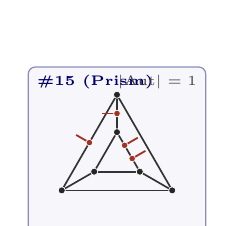
\begin{tikzpicture}[scale=0.88, baseline={(0,0)}]
  \draw[rounded corners=2.5pt, draw=NavyBlue!85!black!45, fill=NavyBlue!85!black!3, line width=0.45pt] (-1.28,-1.18) rectangle (1.28,1.26);
  \node[anchor=north west, font=\tiny\bfseries, text=NavyBlue!85!black, inner sep=1.5pt] at (-1.22,1.21) {\#15 (Prism)};
  \node[anchor=north east, font=\tiny, text=black!75, inner sep=1.5pt] at (1.22,1.21) {$|\mathrm{Aut}|=1$};
  \draw[line width=0.6pt, draw=black!80] (0.000,0.320) -- (0.000,0.860);
  \draw[line width=0.6pt, draw=black!80] (0.000,0.320) -- (0.329,-0.250);
  \draw[line width=0.6pt, draw=black!80] (0.000,0.320) -- (-0.329,-0.250);
  \draw[line width=0.6pt, draw=black!80] (0.000,0.860) -- (-0.797,-0.520);
  \draw[line width=0.6pt, draw=black!80] (0.000,0.860) -- (0.797,-0.520);
  \draw[line width=0.6pt, draw=black!80] (0.329,-0.250) -- (-0.329,-0.250);
  \draw[line width=0.6pt, draw=black!80] (0.329,-0.250) -- (0.797,-0.520);
  \draw[line width=0.6pt, draw=black!80] (-0.329,-0.250) -- (-0.797,-0.520);
  \draw[line width=0.6pt, draw=black!80] (-0.797,-0.520) -- (0.797,-0.520);
  \draw[line width=0.65pt, draw=BrickRed!85!black] (0.000,0.590) -- (-0.220,0.590);
  \filldraw[fill=BrickRed!85!black, draw=white, line width=0.25pt] (0.000,0.590) circle (1.35pt);
  \draw[line width=0.65pt, draw=BrickRed!85!black] (0.110,0.130) -- (0.300,0.240);
  \filldraw[fill=BrickRed!85!black, draw=white, line width=0.25pt] (0.110,0.130) circle (1.35pt);
  \draw[line width=0.65pt, draw=BrickRed!85!black] (0.219,-0.060) -- (0.410,0.050);
  \filldraw[fill=BrickRed!85!black, draw=white, line width=0.25pt] (0.219,-0.060) circle (1.35pt);
  \draw[line width=0.65pt, draw=BrickRed!85!black] (-0.398,0.170) -- (-0.589,0.280);
  \filldraw[fill=BrickRed!85!black, draw=white, line width=0.25pt] (-0.398,0.170) circle (1.35pt);
  \filldraw[fill=black!85, draw=white, line width=0.25pt] (0.000,0.320) circle (1.45pt);
  \filldraw[fill=black!85, draw=white, line width=0.25pt] (-0.329,-0.250) circle (1.45pt);
  \filldraw[fill=black!85, draw=white, line width=0.25pt] (0.329,-0.250) circle (1.45pt);
  \filldraw[fill=black!85, draw=white, line width=0.25pt] (0.000,0.860) circle (1.45pt);
  \filldraw[fill=black!85, draw=white, line width=0.25pt] (-0.797,-0.520) circle (1.45pt);
  \filldraw[fill=black!85, draw=white, line width=0.25pt] (0.797,-0.520) circle (1.45pt);
\end{tikzpicture} &
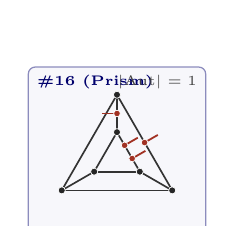
\begin{tikzpicture}[scale=0.88, baseline={(0,0)}]
  \draw[rounded corners=2.5pt, draw=NavyBlue!85!black!45, fill=NavyBlue!85!black!3, line width=0.45pt] (-1.28,-1.18) rectangle (1.28,1.26);
  \node[anchor=north west, font=\tiny\bfseries, text=NavyBlue!85!black, inner sep=1.5pt] at (-1.22,1.21) {\#16 (Prism)};
  \node[anchor=north east, font=\tiny, text=black!75, inner sep=1.5pt] at (1.22,1.21) {$|\mathrm{Aut}|=1$};
  \draw[line width=0.6pt, draw=black!80] (0.000,0.320) -- (0.000,0.860);
  \draw[line width=0.6pt, draw=black!80] (0.000,0.320) -- (0.329,-0.250);
  \draw[line width=0.6pt, draw=black!80] (0.000,0.320) -- (-0.329,-0.250);
  \draw[line width=0.6pt, draw=black!80] (0.000,0.860) -- (-0.797,-0.520);
  \draw[line width=0.6pt, draw=black!80] (0.000,0.860) -- (0.797,-0.520);
  \draw[line width=0.6pt, draw=black!80] (0.329,-0.250) -- (-0.329,-0.250);
  \draw[line width=0.6pt, draw=black!80] (0.329,-0.250) -- (0.797,-0.520);
  \draw[line width=0.6pt, draw=black!80] (-0.329,-0.250) -- (-0.797,-0.520);
  \draw[line width=0.6pt, draw=black!80] (-0.797,-0.520) -- (0.797,-0.520);
  \draw[line width=0.65pt, draw=BrickRed!85!black] (0.000,0.590) -- (-0.220,0.590);
  \filldraw[fill=BrickRed!85!black, draw=white, line width=0.25pt] (0.000,0.590) circle (1.35pt);
  \draw[line width=0.65pt, draw=BrickRed!85!black] (0.110,0.130) -- (0.300,0.240);
  \filldraw[fill=BrickRed!85!black, draw=white, line width=0.25pt] (0.110,0.130) circle (1.35pt);
  \draw[line width=0.65pt, draw=BrickRed!85!black] (0.219,-0.060) -- (0.410,0.050);
  \filldraw[fill=BrickRed!85!black, draw=white, line width=0.25pt] (0.219,-0.060) circle (1.35pt);
  \draw[line width=0.65pt, draw=BrickRed!85!black] (0.398,0.170) -- (0.589,0.280);
  \filldraw[fill=BrickRed!85!black, draw=white, line width=0.25pt] (0.398,0.170) circle (1.35pt);
  \filldraw[fill=black!85, draw=white, line width=0.25pt] (0.000,0.320) circle (1.45pt);
  \filldraw[fill=black!85, draw=white, line width=0.25pt] (-0.329,-0.250) circle (1.45pt);
  \filldraw[fill=black!85, draw=white, line width=0.25pt] (0.329,-0.250) circle (1.45pt);
  \filldraw[fill=black!85, draw=white, line width=0.25pt] (0.000,0.860) circle (1.45pt);
  \filldraw[fill=black!85, draw=white, line width=0.25pt] (-0.797,-0.520) circle (1.45pt);
  \filldraw[fill=black!85, draw=white, line width=0.25pt] (0.797,-0.520) circle (1.45pt);
\end{tikzpicture} &
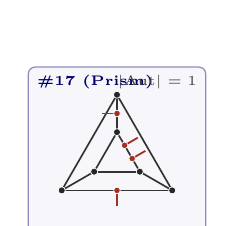
\begin{tikzpicture}[scale=0.88, baseline={(0,0)}]
  \draw[rounded corners=2.5pt, draw=NavyBlue!85!black!45, fill=NavyBlue!85!black!3, line width=0.45pt] (-1.28,-1.18) rectangle (1.28,1.26);
  \node[anchor=north west, font=\tiny\bfseries, text=NavyBlue!85!black, inner sep=1.5pt] at (-1.22,1.21) {\#17 (Prism)};
  \node[anchor=north east, font=\tiny, text=black!75, inner sep=1.5pt] at (1.22,1.21) {$|\mathrm{Aut}|=1$};
  \draw[line width=0.6pt, draw=black!80] (0.000,0.320) -- (0.000,0.860);
  \draw[line width=0.6pt, draw=black!80] (0.000,0.320) -- (0.329,-0.250);
  \draw[line width=0.6pt, draw=black!80] (0.000,0.320) -- (-0.329,-0.250);
  \draw[line width=0.6pt, draw=black!80] (0.000,0.860) -- (-0.797,-0.520);
  \draw[line width=0.6pt, draw=black!80] (0.000,0.860) -- (0.797,-0.520);
  \draw[line width=0.6pt, draw=black!80] (0.329,-0.250) -- (-0.329,-0.250);
  \draw[line width=0.6pt, draw=black!80] (0.329,-0.250) -- (0.797,-0.520);
  \draw[line width=0.6pt, draw=black!80] (-0.329,-0.250) -- (-0.797,-0.520);
  \draw[line width=0.6pt, draw=black!80] (-0.797,-0.520) -- (0.797,-0.520);
  \draw[line width=0.65pt, draw=BrickRed!85!black] (0.000,0.590) -- (-0.220,0.590);
  \filldraw[fill=BrickRed!85!black, draw=white, line width=0.25pt] (0.000,0.590) circle (1.35pt);
  \draw[line width=0.65pt, draw=BrickRed!85!black] (0.110,0.130) -- (0.300,0.240);
  \filldraw[fill=BrickRed!85!black, draw=white, line width=0.25pt] (0.110,0.130) circle (1.35pt);
  \draw[line width=0.65pt, draw=BrickRed!85!black] (0.219,-0.060) -- (0.410,0.050);
  \filldraw[fill=BrickRed!85!black, draw=white, line width=0.25pt] (0.219,-0.060) circle (1.35pt);
  \draw[line width=0.65pt, draw=BrickRed!85!black] (-0.000,-0.520) -- (-0.000,-0.740);
  \filldraw[fill=BrickRed!85!black, draw=white, line width=0.25pt] (-0.000,-0.520) circle (1.35pt);
  \filldraw[fill=black!85, draw=white, line width=0.25pt] (0.000,0.320) circle (1.45pt);
  \filldraw[fill=black!85, draw=white, line width=0.25pt] (-0.329,-0.250) circle (1.45pt);
  \filldraw[fill=black!85, draw=white, line width=0.25pt] (0.329,-0.250) circle (1.45pt);
  \filldraw[fill=black!85, draw=white, line width=0.25pt] (0.000,0.860) circle (1.45pt);
  \filldraw[fill=black!85, draw=white, line width=0.25pt] (-0.797,-0.520) circle (1.45pt);
  \filldraw[fill=black!85, draw=white, line width=0.25pt] (0.797,-0.520) circle (1.45pt);
\end{tikzpicture} &
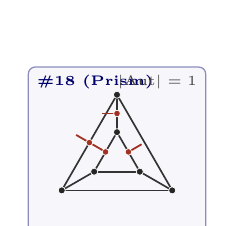
\begin{tikzpicture}[scale=0.88, baseline={(0,0)}]
  \draw[rounded corners=2.5pt, draw=NavyBlue!85!black!45, fill=NavyBlue!85!black!3, line width=0.45pt] (-1.28,-1.18) rectangle (1.28,1.26);
  \node[anchor=north west, font=\tiny\bfseries, text=NavyBlue!85!black, inner sep=1.5pt] at (-1.22,1.21) {\#18 (Prism)};
  \node[anchor=north east, font=\tiny, text=black!75, inner sep=1.5pt] at (1.22,1.21) {$|\mathrm{Aut}|=1$};
  \draw[line width=0.6pt, draw=black!80] (0.000,0.320) -- (0.000,0.860);
  \draw[line width=0.6pt, draw=black!80] (0.000,0.320) -- (0.329,-0.250);
  \draw[line width=0.6pt, draw=black!80] (0.000,0.320) -- (-0.329,-0.250);
  \draw[line width=0.6pt, draw=black!80] (0.000,0.860) -- (-0.797,-0.520);
  \draw[line width=0.6pt, draw=black!80] (0.000,0.860) -- (0.797,-0.520);
  \draw[line width=0.6pt, draw=black!80] (0.329,-0.250) -- (-0.329,-0.250);
  \draw[line width=0.6pt, draw=black!80] (0.329,-0.250) -- (0.797,-0.520);
  \draw[line width=0.6pt, draw=black!80] (-0.329,-0.250) -- (-0.797,-0.520);
  \draw[line width=0.6pt, draw=black!80] (-0.797,-0.520) -- (0.797,-0.520);
  \draw[line width=0.65pt, draw=BrickRed!85!black] (0.000,0.590) -- (-0.220,0.590);
  \filldraw[fill=BrickRed!85!black, draw=white, line width=0.25pt] (0.000,0.590) circle (1.35pt);
  \draw[line width=0.65pt, draw=BrickRed!85!black] (0.165,0.035) -- (0.355,0.145);
  \filldraw[fill=BrickRed!85!black, draw=white, line width=0.25pt] (0.165,0.035) circle (1.35pt);
  \draw[line width=0.65pt, draw=BrickRed!85!black] (-0.165,0.035) -- (-0.355,0.145);
  \filldraw[fill=BrickRed!85!black, draw=white, line width=0.25pt] (-0.165,0.035) circle (1.35pt);
  \draw[line width=0.65pt, draw=BrickRed!85!black] (-0.398,0.170) -- (-0.589,0.280);
  \filldraw[fill=BrickRed!85!black, draw=white, line width=0.25pt] (-0.398,0.170) circle (1.35pt);
  \filldraw[fill=black!85, draw=white, line width=0.25pt] (0.000,0.320) circle (1.45pt);
  \filldraw[fill=black!85, draw=white, line width=0.25pt] (-0.329,-0.250) circle (1.45pt);
  \filldraw[fill=black!85, draw=white, line width=0.25pt] (0.329,-0.250) circle (1.45pt);
  \filldraw[fill=black!85, draw=white, line width=0.25pt] (0.000,0.860) circle (1.45pt);
  \filldraw[fill=black!85, draw=white, line width=0.25pt] (-0.797,-0.520) circle (1.45pt);
  \filldraw[fill=black!85, draw=white, line width=0.25pt] (0.797,-0.520) circle (1.45pt);
\end{tikzpicture} &
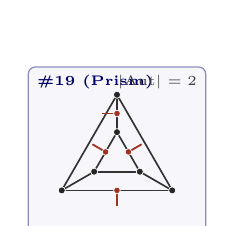
\begin{tikzpicture}[scale=0.88, baseline={(0,0)}]
  \draw[rounded corners=2.5pt, draw=NavyBlue!85!black!45, fill=NavyBlue!85!black!3, line width=0.45pt] (-1.28,-1.18) rectangle (1.28,1.26);
  \node[anchor=north west, font=\tiny\bfseries, text=NavyBlue!85!black, inner sep=1.5pt] at (-1.22,1.21) {\#19 (Prism)};
  \node[anchor=north east, font=\tiny, text=black!75, inner sep=1.5pt] at (1.22,1.21) {$|\mathrm{Aut}|=2$};
  \draw[line width=0.6pt, draw=black!80] (0.000,0.320) -- (0.000,0.860);
  \draw[line width=0.6pt, draw=black!80] (0.000,0.320) -- (0.329,-0.250);
  \draw[line width=0.6pt, draw=black!80] (0.000,0.320) -- (-0.329,-0.250);
  \draw[line width=0.6pt, draw=black!80] (0.000,0.860) -- (-0.797,-0.520);
  \draw[line width=0.6pt, draw=black!80] (0.000,0.860) -- (0.797,-0.520);
  \draw[line width=0.6pt, draw=black!80] (0.329,-0.250) -- (-0.329,-0.250);
  \draw[line width=0.6pt, draw=black!80] (0.329,-0.250) -- (0.797,-0.520);
  \draw[line width=0.6pt, draw=black!80] (-0.329,-0.250) -- (-0.797,-0.520);
  \draw[line width=0.6pt, draw=black!80] (-0.797,-0.520) -- (0.797,-0.520);
  \draw[line width=0.65pt, draw=BrickRed!85!black] (0.000,0.590) -- (-0.220,0.590);
  \filldraw[fill=BrickRed!85!black, draw=white, line width=0.25pt] (0.000,0.590) circle (1.35pt);
  \draw[line width=0.65pt, draw=BrickRed!85!black] (0.165,0.035) -- (0.355,0.145);
  \filldraw[fill=BrickRed!85!black, draw=white, line width=0.25pt] (0.165,0.035) circle (1.35pt);
  \draw[line width=0.65pt, draw=BrickRed!85!black] (-0.165,0.035) -- (-0.355,0.145);
  \filldraw[fill=BrickRed!85!black, draw=white, line width=0.25pt] (-0.165,0.035) circle (1.35pt);
  \draw[line width=0.65pt, draw=BrickRed!85!black] (-0.000,-0.520) -- (-0.000,-0.740);
  \filldraw[fill=BrickRed!85!black, draw=white, line width=0.25pt] (-0.000,-0.520) circle (1.35pt);
  \filldraw[fill=black!85, draw=white, line width=0.25pt] (0.000,0.320) circle (1.45pt);
  \filldraw[fill=black!85, draw=white, line width=0.25pt] (-0.329,-0.250) circle (1.45pt);
  \filldraw[fill=black!85, draw=white, line width=0.25pt] (0.329,-0.250) circle (1.45pt);
  \filldraw[fill=black!85, draw=white, line width=0.25pt] (0.000,0.860) circle (1.45pt);
  \filldraw[fill=black!85, draw=white, line width=0.25pt] (-0.797,-0.520) circle (1.45pt);
  \filldraw[fill=black!85, draw=white, line width=0.25pt] (0.797,-0.520) circle (1.45pt);
\end{tikzpicture} \\[2pt]
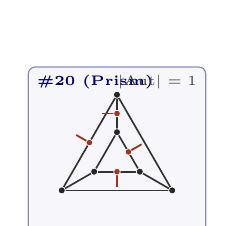
\begin{tikzpicture}[scale=0.88, baseline={(0,0)}]
  \draw[rounded corners=2.5pt, draw=NavyBlue!85!black!45, fill=NavyBlue!85!black!3, line width=0.45pt] (-1.28,-1.18) rectangle (1.28,1.26);
  \node[anchor=north west, font=\tiny\bfseries, text=NavyBlue!85!black, inner sep=1.5pt] at (-1.22,1.21) {\#20 (Prism)};
  \node[anchor=north east, font=\tiny, text=black!75, inner sep=1.5pt] at (1.22,1.21) {$|\mathrm{Aut}|=1$};
  \draw[line width=0.6pt, draw=black!80] (0.000,0.320) -- (0.000,0.860);
  \draw[line width=0.6pt, draw=black!80] (0.000,0.320) -- (0.329,-0.250);
  \draw[line width=0.6pt, draw=black!80] (0.000,0.320) -- (-0.329,-0.250);
  \draw[line width=0.6pt, draw=black!80] (0.000,0.860) -- (-0.797,-0.520);
  \draw[line width=0.6pt, draw=black!80] (0.000,0.860) -- (0.797,-0.520);
  \draw[line width=0.6pt, draw=black!80] (0.329,-0.250) -- (-0.329,-0.250);
  \draw[line width=0.6pt, draw=black!80] (0.329,-0.250) -- (0.797,-0.520);
  \draw[line width=0.6pt, draw=black!80] (-0.329,-0.250) -- (-0.797,-0.520);
  \draw[line width=0.6pt, draw=black!80] (-0.797,-0.520) -- (0.797,-0.520);
  \draw[line width=0.65pt, draw=BrickRed!85!black] (0.000,0.590) -- (-0.220,0.590);
  \filldraw[fill=BrickRed!85!black, draw=white, line width=0.25pt] (0.000,0.590) circle (1.35pt);
  \draw[line width=0.65pt, draw=BrickRed!85!black] (0.165,0.035) -- (0.355,0.145);
  \filldraw[fill=BrickRed!85!black, draw=white, line width=0.25pt] (0.165,0.035) circle (1.35pt);
  \draw[line width=0.65pt, draw=BrickRed!85!black] (-0.398,0.170) -- (-0.589,0.280);
  \filldraw[fill=BrickRed!85!black, draw=white, line width=0.25pt] (-0.398,0.170) circle (1.35pt);
  \draw[line width=0.65pt, draw=BrickRed!85!black] (0.000,-0.250) -- (-0.000,-0.470);
  \filldraw[fill=BrickRed!85!black, draw=white, line width=0.25pt] (0.000,-0.250) circle (1.35pt);
  \filldraw[fill=black!85, draw=white, line width=0.25pt] (0.000,0.320) circle (1.45pt);
  \filldraw[fill=black!85, draw=white, line width=0.25pt] (-0.329,-0.250) circle (1.45pt);
  \filldraw[fill=black!85, draw=white, line width=0.25pt] (0.329,-0.250) circle (1.45pt);
  \filldraw[fill=black!85, draw=white, line width=0.25pt] (0.000,0.860) circle (1.45pt);
  \filldraw[fill=black!85, draw=white, line width=0.25pt] (-0.797,-0.520) circle (1.45pt);
  \filldraw[fill=black!85, draw=white, line width=0.25pt] (0.797,-0.520) circle (1.45pt);
\end{tikzpicture} &
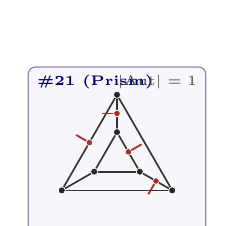
\begin{tikzpicture}[scale=0.88, baseline={(0,0)}]
  \draw[rounded corners=2.5pt, draw=NavyBlue!85!black!45, fill=NavyBlue!85!black!3, line width=0.45pt] (-1.28,-1.18) rectangle (1.28,1.26);
  \node[anchor=north west, font=\tiny\bfseries, text=NavyBlue!85!black, inner sep=1.5pt] at (-1.22,1.21) {\#21 (Prism)};
  \node[anchor=north east, font=\tiny, text=black!75, inner sep=1.5pt] at (1.22,1.21) {$|\mathrm{Aut}|=1$};
  \draw[line width=0.6pt, draw=black!80] (0.000,0.320) -- (0.000,0.860);
  \draw[line width=0.6pt, draw=black!80] (0.000,0.320) -- (0.329,-0.250);
  \draw[line width=0.6pt, draw=black!80] (0.000,0.320) -- (-0.329,-0.250);
  \draw[line width=0.6pt, draw=black!80] (0.000,0.860) -- (-0.797,-0.520);
  \draw[line width=0.6pt, draw=black!80] (0.000,0.860) -- (0.797,-0.520);
  \draw[line width=0.6pt, draw=black!80] (0.329,-0.250) -- (-0.329,-0.250);
  \draw[line width=0.6pt, draw=black!80] (0.329,-0.250) -- (0.797,-0.520);
  \draw[line width=0.6pt, draw=black!80] (-0.329,-0.250) -- (-0.797,-0.520);
  \draw[line width=0.6pt, draw=black!80] (-0.797,-0.520) -- (0.797,-0.520);
  \draw[line width=0.65pt, draw=BrickRed!85!black] (0.000,0.590) -- (-0.220,0.590);
  \filldraw[fill=BrickRed!85!black, draw=white, line width=0.25pt] (0.000,0.590) circle (1.35pt);
  \draw[line width=0.65pt, draw=BrickRed!85!black] (0.165,0.035) -- (0.355,0.145);
  \filldraw[fill=BrickRed!85!black, draw=white, line width=0.25pt] (0.165,0.035) circle (1.35pt);
  \draw[line width=0.65pt, draw=BrickRed!85!black] (-0.398,0.170) -- (-0.589,0.280);
  \filldraw[fill=BrickRed!85!black, draw=white, line width=0.25pt] (-0.398,0.170) circle (1.35pt);
  \draw[line width=0.65pt, draw=BrickRed!85!black] (0.563,-0.385) -- (0.453,-0.576);
  \filldraw[fill=BrickRed!85!black, draw=white, line width=0.25pt] (0.563,-0.385) circle (1.35pt);
  \filldraw[fill=black!85, draw=white, line width=0.25pt] (0.000,0.320) circle (1.45pt);
  \filldraw[fill=black!85, draw=white, line width=0.25pt] (-0.329,-0.250) circle (1.45pt);
  \filldraw[fill=black!85, draw=white, line width=0.25pt] (0.329,-0.250) circle (1.45pt);
  \filldraw[fill=black!85, draw=white, line width=0.25pt] (0.000,0.860) circle (1.45pt);
  \filldraw[fill=black!85, draw=white, line width=0.25pt] (-0.797,-0.520) circle (1.45pt);
  \filldraw[fill=black!85, draw=white, line width=0.25pt] (0.797,-0.520) circle (1.45pt);
\end{tikzpicture} &
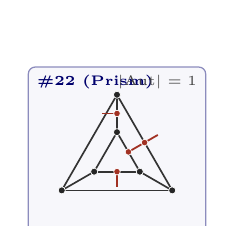
\begin{tikzpicture}[scale=0.88, baseline={(0,0)}]
  \draw[rounded corners=2.5pt, draw=NavyBlue!85!black!45, fill=NavyBlue!85!black!3, line width=0.45pt] (-1.28,-1.18) rectangle (1.28,1.26);
  \node[anchor=north west, font=\tiny\bfseries, text=NavyBlue!85!black, inner sep=1.5pt] at (-1.22,1.21) {\#22 (Prism)};
  \node[anchor=north east, font=\tiny, text=black!75, inner sep=1.5pt] at (1.22,1.21) {$|\mathrm{Aut}|=1$};
  \draw[line width=0.6pt, draw=black!80] (0.000,0.320) -- (0.000,0.860);
  \draw[line width=0.6pt, draw=black!80] (0.000,0.320) -- (0.329,-0.250);
  \draw[line width=0.6pt, draw=black!80] (0.000,0.320) -- (-0.329,-0.250);
  \draw[line width=0.6pt, draw=black!80] (0.000,0.860) -- (-0.797,-0.520);
  \draw[line width=0.6pt, draw=black!80] (0.000,0.860) -- (0.797,-0.520);
  \draw[line width=0.6pt, draw=black!80] (0.329,-0.250) -- (-0.329,-0.250);
  \draw[line width=0.6pt, draw=black!80] (0.329,-0.250) -- (0.797,-0.520);
  \draw[line width=0.6pt, draw=black!80] (-0.329,-0.250) -- (-0.797,-0.520);
  \draw[line width=0.6pt, draw=black!80] (-0.797,-0.520) -- (0.797,-0.520);
  \draw[line width=0.65pt, draw=BrickRed!85!black] (0.000,0.590) -- (-0.220,0.590);
  \filldraw[fill=BrickRed!85!black, draw=white, line width=0.25pt] (0.000,0.590) circle (1.35pt);
  \draw[line width=0.65pt, draw=BrickRed!85!black] (0.165,0.035) -- (0.355,0.145);
  \filldraw[fill=BrickRed!85!black, draw=white, line width=0.25pt] (0.165,0.035) circle (1.35pt);
  \draw[line width=0.65pt, draw=BrickRed!85!black] (0.398,0.170) -- (0.589,0.280);
  \filldraw[fill=BrickRed!85!black, draw=white, line width=0.25pt] (0.398,0.170) circle (1.35pt);
  \draw[line width=0.65pt, draw=BrickRed!85!black] (0.000,-0.250) -- (-0.000,-0.470);
  \filldraw[fill=BrickRed!85!black, draw=white, line width=0.25pt] (0.000,-0.250) circle (1.35pt);
  \filldraw[fill=black!85, draw=white, line width=0.25pt] (0.000,0.320) circle (1.45pt);
  \filldraw[fill=black!85, draw=white, line width=0.25pt] (-0.329,-0.250) circle (1.45pt);
  \filldraw[fill=black!85, draw=white, line width=0.25pt] (0.329,-0.250) circle (1.45pt);
  \filldraw[fill=black!85, draw=white, line width=0.25pt] (0.000,0.860) circle (1.45pt);
  \filldraw[fill=black!85, draw=white, line width=0.25pt] (-0.797,-0.520) circle (1.45pt);
  \filldraw[fill=black!85, draw=white, line width=0.25pt] (0.797,-0.520) circle (1.45pt);
\end{tikzpicture} &
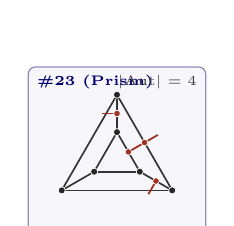
\begin{tikzpicture}[scale=0.88, baseline={(0,0)}]
  \draw[rounded corners=2.5pt, draw=NavyBlue!85!black!45, fill=NavyBlue!85!black!3, line width=0.45pt] (-1.28,-1.18) rectangle (1.28,1.26);
  \node[anchor=north west, font=\tiny\bfseries, text=NavyBlue!85!black, inner sep=1.5pt] at (-1.22,1.21) {\#23 (Prism)};
  \node[anchor=north east, font=\tiny, text=black!75, inner sep=1.5pt] at (1.22,1.21) {$|\mathrm{Aut}|=4$};
  \draw[line width=0.6pt, draw=black!80] (0.000,0.320) -- (0.000,0.860);
  \draw[line width=0.6pt, draw=black!80] (0.000,0.320) -- (0.329,-0.250);
  \draw[line width=0.6pt, draw=black!80] (0.000,0.320) -- (-0.329,-0.250);
  \draw[line width=0.6pt, draw=black!80] (0.000,0.860) -- (-0.797,-0.520);
  \draw[line width=0.6pt, draw=black!80] (0.000,0.860) -- (0.797,-0.520);
  \draw[line width=0.6pt, draw=black!80] (0.329,-0.250) -- (-0.329,-0.250);
  \draw[line width=0.6pt, draw=black!80] (0.329,-0.250) -- (0.797,-0.520);
  \draw[line width=0.6pt, draw=black!80] (-0.329,-0.250) -- (-0.797,-0.520);
  \draw[line width=0.6pt, draw=black!80] (-0.797,-0.520) -- (0.797,-0.520);
  \draw[line width=0.65pt, draw=BrickRed!85!black] (0.000,0.590) -- (-0.220,0.590);
  \filldraw[fill=BrickRed!85!black, draw=white, line width=0.25pt] (0.000,0.590) circle (1.35pt);
  \draw[line width=0.65pt, draw=BrickRed!85!black] (0.165,0.035) -- (0.355,0.145);
  \filldraw[fill=BrickRed!85!black, draw=white, line width=0.25pt] (0.165,0.035) circle (1.35pt);
  \draw[line width=0.65pt, draw=BrickRed!85!black] (0.398,0.170) -- (0.589,0.280);
  \filldraw[fill=BrickRed!85!black, draw=white, line width=0.25pt] (0.398,0.170) circle (1.35pt);
  \draw[line width=0.65pt, draw=BrickRed!85!black] (0.563,-0.385) -- (0.453,-0.576);
  \filldraw[fill=BrickRed!85!black, draw=white, line width=0.25pt] (0.563,-0.385) circle (1.35pt);
  \filldraw[fill=black!85, draw=white, line width=0.25pt] (0.000,0.320) circle (1.45pt);
  \filldraw[fill=black!85, draw=white, line width=0.25pt] (-0.329,-0.250) circle (1.45pt);
  \filldraw[fill=black!85, draw=white, line width=0.25pt] (0.329,-0.250) circle (1.45pt);
  \filldraw[fill=black!85, draw=white, line width=0.25pt] (0.000,0.860) circle (1.45pt);
  \filldraw[fill=black!85, draw=white, line width=0.25pt] (-0.797,-0.520) circle (1.45pt);
  \filldraw[fill=black!85, draw=white, line width=0.25pt] (0.797,-0.520) circle (1.45pt);
\end{tikzpicture} &
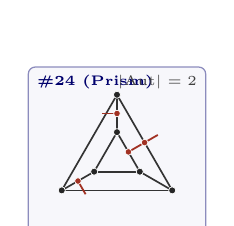
\begin{tikzpicture}[scale=0.88, baseline={(0,0)}]
  \draw[rounded corners=2.5pt, draw=NavyBlue!85!black!45, fill=NavyBlue!85!black!3, line width=0.45pt] (-1.28,-1.18) rectangle (1.28,1.26);
  \node[anchor=north west, font=\tiny\bfseries, text=NavyBlue!85!black, inner sep=1.5pt] at (-1.22,1.21) {\#24 (Prism)};
  \node[anchor=north east, font=\tiny, text=black!75, inner sep=1.5pt] at (1.22,1.21) {$|\mathrm{Aut}|=2$};
  \draw[line width=0.6pt, draw=black!80] (0.000,0.320) -- (0.000,0.860);
  \draw[line width=0.6pt, draw=black!80] (0.000,0.320) -- (0.329,-0.250);
  \draw[line width=0.6pt, draw=black!80] (0.000,0.320) -- (-0.329,-0.250);
  \draw[line width=0.6pt, draw=black!80] (0.000,0.860) -- (-0.797,-0.520);
  \draw[line width=0.6pt, draw=black!80] (0.000,0.860) -- (0.797,-0.520);
  \draw[line width=0.6pt, draw=black!80] (0.329,-0.250) -- (-0.329,-0.250);
  \draw[line width=0.6pt, draw=black!80] (0.329,-0.250) -- (0.797,-0.520);
  \draw[line width=0.6pt, draw=black!80] (-0.329,-0.250) -- (-0.797,-0.520);
  \draw[line width=0.6pt, draw=black!80] (-0.797,-0.520) -- (0.797,-0.520);
  \draw[line width=0.65pt, draw=BrickRed!85!black] (0.000,0.590) -- (-0.220,0.590);
  \filldraw[fill=BrickRed!85!black, draw=white, line width=0.25pt] (0.000,0.590) circle (1.35pt);
  \draw[line width=0.65pt, draw=BrickRed!85!black] (0.165,0.035) -- (0.355,0.145);
  \filldraw[fill=BrickRed!85!black, draw=white, line width=0.25pt] (0.165,0.035) circle (1.35pt);
  \draw[line width=0.65pt, draw=BrickRed!85!black] (0.398,0.170) -- (0.589,0.280);
  \filldraw[fill=BrickRed!85!black, draw=white, line width=0.25pt] (0.398,0.170) circle (1.35pt);
  \draw[line width=0.65pt, draw=BrickRed!85!black] (-0.563,-0.385) -- (-0.453,-0.576);
  \filldraw[fill=BrickRed!85!black, draw=white, line width=0.25pt] (-0.563,-0.385) circle (1.35pt);
  \filldraw[fill=black!85, draw=white, line width=0.25pt] (0.000,0.320) circle (1.45pt);
  \filldraw[fill=black!85, draw=white, line width=0.25pt] (-0.329,-0.250) circle (1.45pt);
  \filldraw[fill=black!85, draw=white, line width=0.25pt] (0.329,-0.250) circle (1.45pt);
  \filldraw[fill=black!85, draw=white, line width=0.25pt] (0.000,0.860) circle (1.45pt);
  \filldraw[fill=black!85, draw=white, line width=0.25pt] (-0.797,-0.520) circle (1.45pt);
  \filldraw[fill=black!85, draw=white, line width=0.25pt] (0.797,-0.520) circle (1.45pt);
\end{tikzpicture} \\[2pt]
\end{tabular}
\caption{Complete bare four-loop Feynman diagram atlas on $\mathbb{R}\times\mathbb{C}^2$, Part~I: Graphs \texttt{\#00}--\texttt{\#24} (comprising all $3$ series--parallel topologies \texttt{\#00}--\texttt{\#02}, all $8$ doubled-kite topologies \texttt{\#03}--\texttt{\#10}, and triangular-prism topologies \texttt{\#11}--\texttt{\#24}). Black nodes denote internal trivalent $f_{ABC}$ vertices ($6$ per graph); crimson nodes with outward stubs denote the $4$ bivalent external superfield insertions $\mathcal{A}$.}
\label{fig:atlas-00-24}
\end{figure}

\begin{figure}[H]
\centering
\setlength{\tabcolsep}{2.2pt}
\renewcommand{\arraystretch}{1.05}
\begin{tabular}{@{}ccccc@{}}
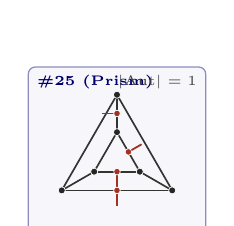
\begin{tikzpicture}[scale=0.88, baseline={(0,0)}]
  \draw[rounded corners=2.5pt, draw=NavyBlue!85!black!45, fill=NavyBlue!85!black!3, line width=0.45pt] (-1.28,-1.18) rectangle (1.28,1.26);
  \node[anchor=north west, font=\tiny\bfseries, text=NavyBlue!85!black, inner sep=1.5pt] at (-1.22,1.21) {\#25 (Prism)};
  \node[anchor=north east, font=\tiny, text=black!75, inner sep=1.5pt] at (1.22,1.21) {$|\mathrm{Aut}|=1$};
  \draw[line width=0.6pt, draw=black!80] (0.000,0.320) -- (0.000,0.860);
  \draw[line width=0.6pt, draw=black!80] (0.000,0.320) -- (0.329,-0.250);
  \draw[line width=0.6pt, draw=black!80] (0.000,0.320) -- (-0.329,-0.250);
  \draw[line width=0.6pt, draw=black!80] (0.000,0.860) -- (-0.797,-0.520);
  \draw[line width=0.6pt, draw=black!80] (0.000,0.860) -- (0.797,-0.520);
  \draw[line width=0.6pt, draw=black!80] (0.329,-0.250) -- (-0.329,-0.250);
  \draw[line width=0.6pt, draw=black!80] (0.329,-0.250) -- (0.797,-0.520);
  \draw[line width=0.6pt, draw=black!80] (-0.329,-0.250) -- (-0.797,-0.520);
  \draw[line width=0.6pt, draw=black!80] (-0.797,-0.520) -- (0.797,-0.520);
  \draw[line width=0.65pt, draw=BrickRed!85!black] (0.000,0.590) -- (-0.220,0.590);
  \filldraw[fill=BrickRed!85!black, draw=white, line width=0.25pt] (0.000,0.590) circle (1.35pt);
  \draw[line width=0.65pt, draw=BrickRed!85!black] (0.165,0.035) -- (0.355,0.145);
  \filldraw[fill=BrickRed!85!black, draw=white, line width=0.25pt] (0.165,0.035) circle (1.35pt);
  \draw[line width=0.65pt, draw=BrickRed!85!black] (0.000,-0.250) -- (-0.000,-0.470);
  \filldraw[fill=BrickRed!85!black, draw=white, line width=0.25pt] (0.000,-0.250) circle (1.35pt);
  \draw[line width=0.65pt, draw=BrickRed!85!black] (-0.000,-0.520) -- (-0.000,-0.740);
  \filldraw[fill=BrickRed!85!black, draw=white, line width=0.25pt] (-0.000,-0.520) circle (1.35pt);
  \filldraw[fill=black!85, draw=white, line width=0.25pt] (0.000,0.320) circle (1.45pt);
  \filldraw[fill=black!85, draw=white, line width=0.25pt] (-0.329,-0.250) circle (1.45pt);
  \filldraw[fill=black!85, draw=white, line width=0.25pt] (0.329,-0.250) circle (1.45pt);
  \filldraw[fill=black!85, draw=white, line width=0.25pt] (0.000,0.860) circle (1.45pt);
  \filldraw[fill=black!85, draw=white, line width=0.25pt] (-0.797,-0.520) circle (1.45pt);
  \filldraw[fill=black!85, draw=white, line width=0.25pt] (0.797,-0.520) circle (1.45pt);
\end{tikzpicture} &
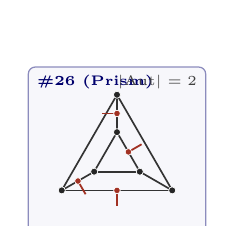
\begin{tikzpicture}[scale=0.88, baseline={(0,0)}]
  \draw[rounded corners=2.5pt, draw=NavyBlue!85!black!45, fill=NavyBlue!85!black!3, line width=0.45pt] (-1.28,-1.18) rectangle (1.28,1.26);
  \node[anchor=north west, font=\tiny\bfseries, text=NavyBlue!85!black, inner sep=1.5pt] at (-1.22,1.21) {\#26 (Prism)};
  \node[anchor=north east, font=\tiny, text=black!75, inner sep=1.5pt] at (1.22,1.21) {$|\mathrm{Aut}|=2$};
  \draw[line width=0.6pt, draw=black!80] (0.000,0.320) -- (0.000,0.860);
  \draw[line width=0.6pt, draw=black!80] (0.000,0.320) -- (0.329,-0.250);
  \draw[line width=0.6pt, draw=black!80] (0.000,0.320) -- (-0.329,-0.250);
  \draw[line width=0.6pt, draw=black!80] (0.000,0.860) -- (-0.797,-0.520);
  \draw[line width=0.6pt, draw=black!80] (0.000,0.860) -- (0.797,-0.520);
  \draw[line width=0.6pt, draw=black!80] (0.329,-0.250) -- (-0.329,-0.250);
  \draw[line width=0.6pt, draw=black!80] (0.329,-0.250) -- (0.797,-0.520);
  \draw[line width=0.6pt, draw=black!80] (-0.329,-0.250) -- (-0.797,-0.520);
  \draw[line width=0.6pt, draw=black!80] (-0.797,-0.520) -- (0.797,-0.520);
  \draw[line width=0.65pt, draw=BrickRed!85!black] (0.000,0.590) -- (-0.220,0.590);
  \filldraw[fill=BrickRed!85!black, draw=white, line width=0.25pt] (0.000,0.590) circle (1.35pt);
  \draw[line width=0.65pt, draw=BrickRed!85!black] (0.165,0.035) -- (0.355,0.145);
  \filldraw[fill=BrickRed!85!black, draw=white, line width=0.25pt] (0.165,0.035) circle (1.35pt);
  \draw[line width=0.65pt, draw=BrickRed!85!black] (-0.563,-0.385) -- (-0.453,-0.576);
  \filldraw[fill=BrickRed!85!black, draw=white, line width=0.25pt] (-0.563,-0.385) circle (1.35pt);
  \draw[line width=0.65pt, draw=BrickRed!85!black] (-0.000,-0.520) -- (-0.000,-0.740);
  \filldraw[fill=BrickRed!85!black, draw=white, line width=0.25pt] (-0.000,-0.520) circle (1.35pt);
  \filldraw[fill=black!85, draw=white, line width=0.25pt] (0.000,0.320) circle (1.45pt);
  \filldraw[fill=black!85, draw=white, line width=0.25pt] (-0.329,-0.250) circle (1.45pt);
  \filldraw[fill=black!85, draw=white, line width=0.25pt] (0.329,-0.250) circle (1.45pt);
  \filldraw[fill=black!85, draw=white, line width=0.25pt] (0.000,0.860) circle (1.45pt);
  \filldraw[fill=black!85, draw=white, line width=0.25pt] (-0.797,-0.520) circle (1.45pt);
  \filldraw[fill=black!85, draw=white, line width=0.25pt] (0.797,-0.520) circle (1.45pt);
\end{tikzpicture} &
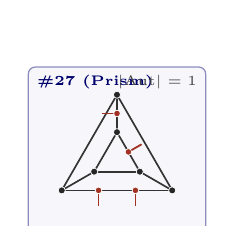
\begin{tikzpicture}[scale=0.88, baseline={(0,0)}]
  \draw[rounded corners=2.5pt, draw=NavyBlue!85!black!45, fill=NavyBlue!85!black!3, line width=0.45pt] (-1.28,-1.18) rectangle (1.28,1.26);
  \node[anchor=north west, font=\tiny\bfseries, text=NavyBlue!85!black, inner sep=1.5pt] at (-1.22,1.21) {\#27 (Prism)};
  \node[anchor=north east, font=\tiny, text=black!75, inner sep=1.5pt] at (1.22,1.21) {$|\mathrm{Aut}|=1$};
  \draw[line width=0.6pt, draw=black!80] (0.000,0.320) -- (0.000,0.860);
  \draw[line width=0.6pt, draw=black!80] (0.000,0.320) -- (0.329,-0.250);
  \draw[line width=0.6pt, draw=black!80] (0.000,0.320) -- (-0.329,-0.250);
  \draw[line width=0.6pt, draw=black!80] (0.000,0.860) -- (-0.797,-0.520);
  \draw[line width=0.6pt, draw=black!80] (0.000,0.860) -- (0.797,-0.520);
  \draw[line width=0.6pt, draw=black!80] (0.329,-0.250) -- (-0.329,-0.250);
  \draw[line width=0.6pt, draw=black!80] (0.329,-0.250) -- (0.797,-0.520);
  \draw[line width=0.6pt, draw=black!80] (-0.329,-0.250) -- (-0.797,-0.520);
  \draw[line width=0.6pt, draw=black!80] (-0.797,-0.520) -- (0.797,-0.520);
  \draw[line width=0.65pt, draw=BrickRed!85!black] (0.000,0.590) -- (-0.220,0.590);
  \filldraw[fill=BrickRed!85!black, draw=white, line width=0.25pt] (0.000,0.590) circle (1.35pt);
  \draw[line width=0.65pt, draw=BrickRed!85!black] (0.165,0.035) -- (0.355,0.145);
  \filldraw[fill=BrickRed!85!black, draw=white, line width=0.25pt] (0.165,0.035) circle (1.35pt);
  \draw[line width=0.65pt, draw=BrickRed!85!black] (-0.266,-0.520) -- (-0.266,-0.740);
  \filldraw[fill=BrickRed!85!black, draw=white, line width=0.25pt] (-0.266,-0.520) circle (1.35pt);
  \draw[line width=0.65pt, draw=BrickRed!85!black] (0.266,-0.520) -- (0.266,-0.740);
  \filldraw[fill=BrickRed!85!black, draw=white, line width=0.25pt] (0.266,-0.520) circle (1.35pt);
  \filldraw[fill=black!85, draw=white, line width=0.25pt] (0.000,0.320) circle (1.45pt);
  \filldraw[fill=black!85, draw=white, line width=0.25pt] (-0.329,-0.250) circle (1.45pt);
  \filldraw[fill=black!85, draw=white, line width=0.25pt] (0.329,-0.250) circle (1.45pt);
  \filldraw[fill=black!85, draw=white, line width=0.25pt] (0.000,0.860) circle (1.45pt);
  \filldraw[fill=black!85, draw=white, line width=0.25pt] (-0.797,-0.520) circle (1.45pt);
  \filldraw[fill=black!85, draw=white, line width=0.25pt] (0.797,-0.520) circle (1.45pt);
\end{tikzpicture} &
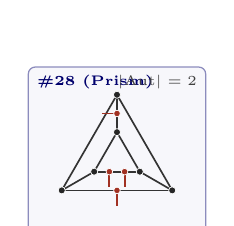
\begin{tikzpicture}[scale=0.88, baseline={(0,0)}]
  \draw[rounded corners=2.5pt, draw=NavyBlue!85!black!45, fill=NavyBlue!85!black!3, line width=0.45pt] (-1.28,-1.18) rectangle (1.28,1.26);
  \node[anchor=north west, font=\tiny\bfseries, text=NavyBlue!85!black, inner sep=1.5pt] at (-1.22,1.21) {\#28 (Prism)};
  \node[anchor=north east, font=\tiny, text=black!75, inner sep=1.5pt] at (1.22,1.21) {$|\mathrm{Aut}|=2$};
  \draw[line width=0.6pt, draw=black!80] (0.000,0.320) -- (0.000,0.860);
  \draw[line width=0.6pt, draw=black!80] (0.000,0.320) -- (0.329,-0.250);
  \draw[line width=0.6pt, draw=black!80] (0.000,0.320) -- (-0.329,-0.250);
  \draw[line width=0.6pt, draw=black!80] (0.000,0.860) -- (-0.797,-0.520);
  \draw[line width=0.6pt, draw=black!80] (0.000,0.860) -- (0.797,-0.520);
  \draw[line width=0.6pt, draw=black!80] (0.329,-0.250) -- (-0.329,-0.250);
  \draw[line width=0.6pt, draw=black!80] (0.329,-0.250) -- (0.797,-0.520);
  \draw[line width=0.6pt, draw=black!80] (-0.329,-0.250) -- (-0.797,-0.520);
  \draw[line width=0.6pt, draw=black!80] (-0.797,-0.520) -- (0.797,-0.520);
  \draw[line width=0.65pt, draw=BrickRed!85!black] (0.000,0.590) -- (-0.220,0.590);
  \filldraw[fill=BrickRed!85!black, draw=white, line width=0.25pt] (0.000,0.590) circle (1.35pt);
  \draw[line width=0.65pt, draw=BrickRed!85!black] (0.110,-0.250) -- (0.110,-0.470);
  \filldraw[fill=BrickRed!85!black, draw=white, line width=0.25pt] (0.110,-0.250) circle (1.35pt);
  \draw[line width=0.65pt, draw=BrickRed!85!black] (-0.110,-0.250) -- (-0.110,-0.470);
  \filldraw[fill=BrickRed!85!black, draw=white, line width=0.25pt] (-0.110,-0.250) circle (1.35pt);
  \draw[line width=0.65pt, draw=BrickRed!85!black] (-0.000,-0.520) -- (-0.000,-0.740);
  \filldraw[fill=BrickRed!85!black, draw=white, line width=0.25pt] (-0.000,-0.520) circle (1.35pt);
  \filldraw[fill=black!85, draw=white, line width=0.25pt] (0.000,0.320) circle (1.45pt);
  \filldraw[fill=black!85, draw=white, line width=0.25pt] (-0.329,-0.250) circle (1.45pt);
  \filldraw[fill=black!85, draw=white, line width=0.25pt] (0.329,-0.250) circle (1.45pt);
  \filldraw[fill=black!85, draw=white, line width=0.25pt] (0.000,0.860) circle (1.45pt);
  \filldraw[fill=black!85, draw=white, line width=0.25pt] (-0.797,-0.520) circle (1.45pt);
  \filldraw[fill=black!85, draw=white, line width=0.25pt] (0.797,-0.520) circle (1.45pt);
\end{tikzpicture} &
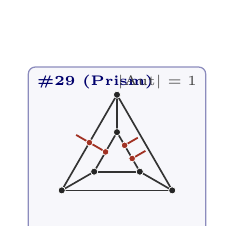
\begin{tikzpicture}[scale=0.88, baseline={(0,0)}]
  \draw[rounded corners=2.5pt, draw=NavyBlue!85!black!45, fill=NavyBlue!85!black!3, line width=0.45pt] (-1.28,-1.18) rectangle (1.28,1.26);
  \node[anchor=north west, font=\tiny\bfseries, text=NavyBlue!85!black, inner sep=1.5pt] at (-1.22,1.21) {\#29 (Prism)};
  \node[anchor=north east, font=\tiny, text=black!75, inner sep=1.5pt] at (1.22,1.21) {$|\mathrm{Aut}|=1$};
  \draw[line width=0.6pt, draw=black!80] (0.000,0.320) -- (0.000,0.860);
  \draw[line width=0.6pt, draw=black!80] (0.000,0.320) -- (0.329,-0.250);
  \draw[line width=0.6pt, draw=black!80] (0.000,0.320) -- (-0.329,-0.250);
  \draw[line width=0.6pt, draw=black!80] (0.000,0.860) -- (-0.797,-0.520);
  \draw[line width=0.6pt, draw=black!80] (0.000,0.860) -- (0.797,-0.520);
  \draw[line width=0.6pt, draw=black!80] (0.329,-0.250) -- (-0.329,-0.250);
  \draw[line width=0.6pt, draw=black!80] (0.329,-0.250) -- (0.797,-0.520);
  \draw[line width=0.6pt, draw=black!80] (-0.329,-0.250) -- (-0.797,-0.520);
  \draw[line width=0.6pt, draw=black!80] (-0.797,-0.520) -- (0.797,-0.520);
  \draw[line width=0.65pt, draw=BrickRed!85!black] (0.110,0.130) -- (0.300,0.240);
  \filldraw[fill=BrickRed!85!black, draw=white, line width=0.25pt] (0.110,0.130) circle (1.35pt);
  \draw[line width=0.65pt, draw=BrickRed!85!black] (0.219,-0.060) -- (0.410,0.050);
  \filldraw[fill=BrickRed!85!black, draw=white, line width=0.25pt] (0.219,-0.060) circle (1.35pt);
  \draw[line width=0.65pt, draw=BrickRed!85!black] (-0.165,0.035) -- (-0.355,0.145);
  \filldraw[fill=BrickRed!85!black, draw=white, line width=0.25pt] (-0.165,0.035) circle (1.35pt);
  \draw[line width=0.65pt, draw=BrickRed!85!black] (-0.398,0.170) -- (-0.589,0.280);
  \filldraw[fill=BrickRed!85!black, draw=white, line width=0.25pt] (-0.398,0.170) circle (1.35pt);
  \filldraw[fill=black!85, draw=white, line width=0.25pt] (0.000,0.320) circle (1.45pt);
  \filldraw[fill=black!85, draw=white, line width=0.25pt] (-0.329,-0.250) circle (1.45pt);
  \filldraw[fill=black!85, draw=white, line width=0.25pt] (0.329,-0.250) circle (1.45pt);
  \filldraw[fill=black!85, draw=white, line width=0.25pt] (0.000,0.860) circle (1.45pt);
  \filldraw[fill=black!85, draw=white, line width=0.25pt] (-0.797,-0.520) circle (1.45pt);
  \filldraw[fill=black!85, draw=white, line width=0.25pt] (0.797,-0.520) circle (1.45pt);
\end{tikzpicture} \\[2pt]
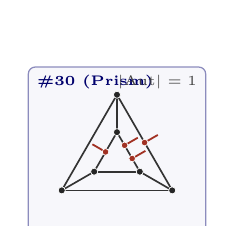
\begin{tikzpicture}[scale=0.88, baseline={(0,0)}]
  \draw[rounded corners=2.5pt, draw=NavyBlue!85!black!45, fill=NavyBlue!85!black!3, line width=0.45pt] (-1.28,-1.18) rectangle (1.28,1.26);
  \node[anchor=north west, font=\tiny\bfseries, text=NavyBlue!85!black, inner sep=1.5pt] at (-1.22,1.21) {\#30 (Prism)};
  \node[anchor=north east, font=\tiny, text=black!75, inner sep=1.5pt] at (1.22,1.21) {$|\mathrm{Aut}|=1$};
  \draw[line width=0.6pt, draw=black!80] (0.000,0.320) -- (0.000,0.860);
  \draw[line width=0.6pt, draw=black!80] (0.000,0.320) -- (0.329,-0.250);
  \draw[line width=0.6pt, draw=black!80] (0.000,0.320) -- (-0.329,-0.250);
  \draw[line width=0.6pt, draw=black!80] (0.000,0.860) -- (-0.797,-0.520);
  \draw[line width=0.6pt, draw=black!80] (0.000,0.860) -- (0.797,-0.520);
  \draw[line width=0.6pt, draw=black!80] (0.329,-0.250) -- (-0.329,-0.250);
  \draw[line width=0.6pt, draw=black!80] (0.329,-0.250) -- (0.797,-0.520);
  \draw[line width=0.6pt, draw=black!80] (-0.329,-0.250) -- (-0.797,-0.520);
  \draw[line width=0.6pt, draw=black!80] (-0.797,-0.520) -- (0.797,-0.520);
  \draw[line width=0.65pt, draw=BrickRed!85!black] (0.110,0.130) -- (0.300,0.240);
  \filldraw[fill=BrickRed!85!black, draw=white, line width=0.25pt] (0.110,0.130) circle (1.35pt);
  \draw[line width=0.65pt, draw=BrickRed!85!black] (0.219,-0.060) -- (0.410,0.050);
  \filldraw[fill=BrickRed!85!black, draw=white, line width=0.25pt] (0.219,-0.060) circle (1.35pt);
  \draw[line width=0.65pt, draw=BrickRed!85!black] (-0.165,0.035) -- (-0.355,0.145);
  \filldraw[fill=BrickRed!85!black, draw=white, line width=0.25pt] (-0.165,0.035) circle (1.35pt);
  \draw[line width=0.65pt, draw=BrickRed!85!black] (0.398,0.170) -- (0.589,0.280);
  \filldraw[fill=BrickRed!85!black, draw=white, line width=0.25pt] (0.398,0.170) circle (1.35pt);
  \filldraw[fill=black!85, draw=white, line width=0.25pt] (0.000,0.320) circle (1.45pt);
  \filldraw[fill=black!85, draw=white, line width=0.25pt] (-0.329,-0.250) circle (1.45pt);
  \filldraw[fill=black!85, draw=white, line width=0.25pt] (0.329,-0.250) circle (1.45pt);
  \filldraw[fill=black!85, draw=white, line width=0.25pt] (0.000,0.860) circle (1.45pt);
  \filldraw[fill=black!85, draw=white, line width=0.25pt] (-0.797,-0.520) circle (1.45pt);
  \filldraw[fill=black!85, draw=white, line width=0.25pt] (0.797,-0.520) circle (1.45pt);
\end{tikzpicture} &
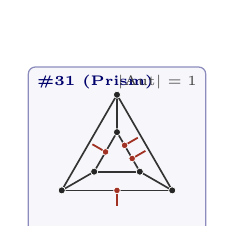
\begin{tikzpicture}[scale=0.88, baseline={(0,0)}]
  \draw[rounded corners=2.5pt, draw=NavyBlue!85!black!45, fill=NavyBlue!85!black!3, line width=0.45pt] (-1.28,-1.18) rectangle (1.28,1.26);
  \node[anchor=north west, font=\tiny\bfseries, text=NavyBlue!85!black, inner sep=1.5pt] at (-1.22,1.21) {\#31 (Prism)};
  \node[anchor=north east, font=\tiny, text=black!75, inner sep=1.5pt] at (1.22,1.21) {$|\mathrm{Aut}|=1$};
  \draw[line width=0.6pt, draw=black!80] (0.000,0.320) -- (0.000,0.860);
  \draw[line width=0.6pt, draw=black!80] (0.000,0.320) -- (0.329,-0.250);
  \draw[line width=0.6pt, draw=black!80] (0.000,0.320) -- (-0.329,-0.250);
  \draw[line width=0.6pt, draw=black!80] (0.000,0.860) -- (-0.797,-0.520);
  \draw[line width=0.6pt, draw=black!80] (0.000,0.860) -- (0.797,-0.520);
  \draw[line width=0.6pt, draw=black!80] (0.329,-0.250) -- (-0.329,-0.250);
  \draw[line width=0.6pt, draw=black!80] (0.329,-0.250) -- (0.797,-0.520);
  \draw[line width=0.6pt, draw=black!80] (-0.329,-0.250) -- (-0.797,-0.520);
  \draw[line width=0.6pt, draw=black!80] (-0.797,-0.520) -- (0.797,-0.520);
  \draw[line width=0.65pt, draw=BrickRed!85!black] (0.110,0.130) -- (0.300,0.240);
  \filldraw[fill=BrickRed!85!black, draw=white, line width=0.25pt] (0.110,0.130) circle (1.35pt);
  \draw[line width=0.65pt, draw=BrickRed!85!black] (0.219,-0.060) -- (0.410,0.050);
  \filldraw[fill=BrickRed!85!black, draw=white, line width=0.25pt] (0.219,-0.060) circle (1.35pt);
  \draw[line width=0.65pt, draw=BrickRed!85!black] (-0.165,0.035) -- (-0.355,0.145);
  \filldraw[fill=BrickRed!85!black, draw=white, line width=0.25pt] (-0.165,0.035) circle (1.35pt);
  \draw[line width=0.65pt, draw=BrickRed!85!black] (-0.000,-0.520) -- (-0.000,-0.740);
  \filldraw[fill=BrickRed!85!black, draw=white, line width=0.25pt] (-0.000,-0.520) circle (1.35pt);
  \filldraw[fill=black!85, draw=white, line width=0.25pt] (0.000,0.320) circle (1.45pt);
  \filldraw[fill=black!85, draw=white, line width=0.25pt] (-0.329,-0.250) circle (1.45pt);
  \filldraw[fill=black!85, draw=white, line width=0.25pt] (0.329,-0.250) circle (1.45pt);
  \filldraw[fill=black!85, draw=white, line width=0.25pt] (0.000,0.860) circle (1.45pt);
  \filldraw[fill=black!85, draw=white, line width=0.25pt] (-0.797,-0.520) circle (1.45pt);
  \filldraw[fill=black!85, draw=white, line width=0.25pt] (0.797,-0.520) circle (1.45pt);
\end{tikzpicture} &
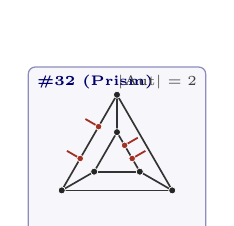
\begin{tikzpicture}[scale=0.88, baseline={(0,0)}]
  \draw[rounded corners=2.5pt, draw=NavyBlue!85!black!45, fill=NavyBlue!85!black!3, line width=0.45pt] (-1.28,-1.18) rectangle (1.28,1.26);
  \node[anchor=north west, font=\tiny\bfseries, text=NavyBlue!85!black, inner sep=1.5pt] at (-1.22,1.21) {\#32 (Prism)};
  \node[anchor=north east, font=\tiny, text=black!75, inner sep=1.5pt] at (1.22,1.21) {$|\mathrm{Aut}|=2$};
  \draw[line width=0.6pt, draw=black!80] (0.000,0.320) -- (0.000,0.860);
  \draw[line width=0.6pt, draw=black!80] (0.000,0.320) -- (0.329,-0.250);
  \draw[line width=0.6pt, draw=black!80] (0.000,0.320) -- (-0.329,-0.250);
  \draw[line width=0.6pt, draw=black!80] (0.000,0.860) -- (-0.797,-0.520);
  \draw[line width=0.6pt, draw=black!80] (0.000,0.860) -- (0.797,-0.520);
  \draw[line width=0.6pt, draw=black!80] (0.329,-0.250) -- (-0.329,-0.250);
  \draw[line width=0.6pt, draw=black!80] (0.329,-0.250) -- (0.797,-0.520);
  \draw[line width=0.6pt, draw=black!80] (-0.329,-0.250) -- (-0.797,-0.520);
  \draw[line width=0.6pt, draw=black!80] (-0.797,-0.520) -- (0.797,-0.520);
  \draw[line width=0.65pt, draw=BrickRed!85!black] (0.110,0.130) -- (0.300,0.240);
  \filldraw[fill=BrickRed!85!black, draw=white, line width=0.25pt] (0.110,0.130) circle (1.35pt);
  \draw[line width=0.65pt, draw=BrickRed!85!black] (0.219,-0.060) -- (0.410,0.050);
  \filldraw[fill=BrickRed!85!black, draw=white, line width=0.25pt] (0.219,-0.060) circle (1.35pt);
  \draw[line width=0.65pt, draw=BrickRed!85!black] (-0.266,0.400) -- (-0.456,0.510);
  \filldraw[fill=BrickRed!85!black, draw=white, line width=0.25pt] (-0.266,0.400) circle (1.35pt);
  \draw[line width=0.65pt, draw=BrickRed!85!black] (-0.531,-0.060) -- (-0.722,0.050);
  \filldraw[fill=BrickRed!85!black, draw=white, line width=0.25pt] (-0.531,-0.060) circle (1.35pt);
  \filldraw[fill=black!85, draw=white, line width=0.25pt] (0.000,0.320) circle (1.45pt);
  \filldraw[fill=black!85, draw=white, line width=0.25pt] (-0.329,-0.250) circle (1.45pt);
  \filldraw[fill=black!85, draw=white, line width=0.25pt] (0.329,-0.250) circle (1.45pt);
  \filldraw[fill=black!85, draw=white, line width=0.25pt] (0.000,0.860) circle (1.45pt);
  \filldraw[fill=black!85, draw=white, line width=0.25pt] (-0.797,-0.520) circle (1.45pt);
  \filldraw[fill=black!85, draw=white, line width=0.25pt] (0.797,-0.520) circle (1.45pt);
\end{tikzpicture} &
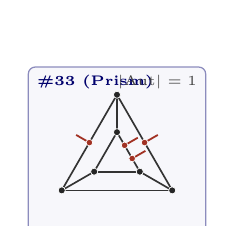
\begin{tikzpicture}[scale=0.88, baseline={(0,0)}]
  \draw[rounded corners=2.5pt, draw=NavyBlue!85!black!45, fill=NavyBlue!85!black!3, line width=0.45pt] (-1.28,-1.18) rectangle (1.28,1.26);
  \node[anchor=north west, font=\tiny\bfseries, text=NavyBlue!85!black, inner sep=1.5pt] at (-1.22,1.21) {\#33 (Prism)};
  \node[anchor=north east, font=\tiny, text=black!75, inner sep=1.5pt] at (1.22,1.21) {$|\mathrm{Aut}|=1$};
  \draw[line width=0.6pt, draw=black!80] (0.000,0.320) -- (0.000,0.860);
  \draw[line width=0.6pt, draw=black!80] (0.000,0.320) -- (0.329,-0.250);
  \draw[line width=0.6pt, draw=black!80] (0.000,0.320) -- (-0.329,-0.250);
  \draw[line width=0.6pt, draw=black!80] (0.000,0.860) -- (-0.797,-0.520);
  \draw[line width=0.6pt, draw=black!80] (0.000,0.860) -- (0.797,-0.520);
  \draw[line width=0.6pt, draw=black!80] (0.329,-0.250) -- (-0.329,-0.250);
  \draw[line width=0.6pt, draw=black!80] (0.329,-0.250) -- (0.797,-0.520);
  \draw[line width=0.6pt, draw=black!80] (-0.329,-0.250) -- (-0.797,-0.520);
  \draw[line width=0.6pt, draw=black!80] (-0.797,-0.520) -- (0.797,-0.520);
  \draw[line width=0.65pt, draw=BrickRed!85!black] (0.110,0.130) -- (0.300,0.240);
  \filldraw[fill=BrickRed!85!black, draw=white, line width=0.25pt] (0.110,0.130) circle (1.35pt);
  \draw[line width=0.65pt, draw=BrickRed!85!black] (0.219,-0.060) -- (0.410,0.050);
  \filldraw[fill=BrickRed!85!black, draw=white, line width=0.25pt] (0.219,-0.060) circle (1.35pt);
  \draw[line width=0.65pt, draw=BrickRed!85!black] (-0.398,0.170) -- (-0.589,0.280);
  \filldraw[fill=BrickRed!85!black, draw=white, line width=0.25pt] (-0.398,0.170) circle (1.35pt);
  \draw[line width=0.65pt, draw=BrickRed!85!black] (0.398,0.170) -- (0.589,0.280);
  \filldraw[fill=BrickRed!85!black, draw=white, line width=0.25pt] (0.398,0.170) circle (1.35pt);
  \filldraw[fill=black!85, draw=white, line width=0.25pt] (0.000,0.320) circle (1.45pt);
  \filldraw[fill=black!85, draw=white, line width=0.25pt] (-0.329,-0.250) circle (1.45pt);
  \filldraw[fill=black!85, draw=white, line width=0.25pt] (0.329,-0.250) circle (1.45pt);
  \filldraw[fill=black!85, draw=white, line width=0.25pt] (0.000,0.860) circle (1.45pt);
  \filldraw[fill=black!85, draw=white, line width=0.25pt] (-0.797,-0.520) circle (1.45pt);
  \filldraw[fill=black!85, draw=white, line width=0.25pt] (0.797,-0.520) circle (1.45pt);
\end{tikzpicture} &
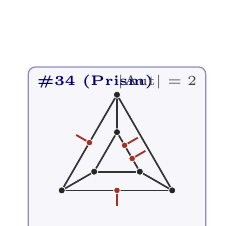
\begin{tikzpicture}[scale=0.88, baseline={(0,0)}]
  \draw[rounded corners=2.5pt, draw=NavyBlue!85!black!45, fill=NavyBlue!85!black!3, line width=0.45pt] (-1.28,-1.18) rectangle (1.28,1.26);
  \node[anchor=north west, font=\tiny\bfseries, text=NavyBlue!85!black, inner sep=1.5pt] at (-1.22,1.21) {\#34 (Prism)};
  \node[anchor=north east, font=\tiny, text=black!75, inner sep=1.5pt] at (1.22,1.21) {$|\mathrm{Aut}|=2$};
  \draw[line width=0.6pt, draw=black!80] (0.000,0.320) -- (0.000,0.860);
  \draw[line width=0.6pt, draw=black!80] (0.000,0.320) -- (0.329,-0.250);
  \draw[line width=0.6pt, draw=black!80] (0.000,0.320) -- (-0.329,-0.250);
  \draw[line width=0.6pt, draw=black!80] (0.000,0.860) -- (-0.797,-0.520);
  \draw[line width=0.6pt, draw=black!80] (0.000,0.860) -- (0.797,-0.520);
  \draw[line width=0.6pt, draw=black!80] (0.329,-0.250) -- (-0.329,-0.250);
  \draw[line width=0.6pt, draw=black!80] (0.329,-0.250) -- (0.797,-0.520);
  \draw[line width=0.6pt, draw=black!80] (-0.329,-0.250) -- (-0.797,-0.520);
  \draw[line width=0.6pt, draw=black!80] (-0.797,-0.520) -- (0.797,-0.520);
  \draw[line width=0.65pt, draw=BrickRed!85!black] (0.110,0.130) -- (0.300,0.240);
  \filldraw[fill=BrickRed!85!black, draw=white, line width=0.25pt] (0.110,0.130) circle (1.35pt);
  \draw[line width=0.65pt, draw=BrickRed!85!black] (0.219,-0.060) -- (0.410,0.050);
  \filldraw[fill=BrickRed!85!black, draw=white, line width=0.25pt] (0.219,-0.060) circle (1.35pt);
  \draw[line width=0.65pt, draw=BrickRed!85!black] (-0.398,0.170) -- (-0.589,0.280);
  \filldraw[fill=BrickRed!85!black, draw=white, line width=0.25pt] (-0.398,0.170) circle (1.35pt);
  \draw[line width=0.65pt, draw=BrickRed!85!black] (-0.000,-0.520) -- (-0.000,-0.740);
  \filldraw[fill=BrickRed!85!black, draw=white, line width=0.25pt] (-0.000,-0.520) circle (1.35pt);
  \filldraw[fill=black!85, draw=white, line width=0.25pt] (0.000,0.320) circle (1.45pt);
  \filldraw[fill=black!85, draw=white, line width=0.25pt] (-0.329,-0.250) circle (1.45pt);
  \filldraw[fill=black!85, draw=white, line width=0.25pt] (0.329,-0.250) circle (1.45pt);
  \filldraw[fill=black!85, draw=white, line width=0.25pt] (0.000,0.860) circle (1.45pt);
  \filldraw[fill=black!85, draw=white, line width=0.25pt] (-0.797,-0.520) circle (1.45pt);
  \filldraw[fill=black!85, draw=white, line width=0.25pt] (0.797,-0.520) circle (1.45pt);
\end{tikzpicture} \\[2pt]
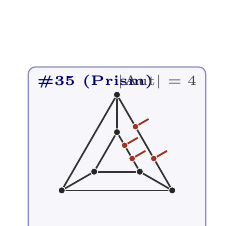
\begin{tikzpicture}[scale=0.88, baseline={(0,0)}]
  \draw[rounded corners=2.5pt, draw=NavyBlue!85!black!45, fill=NavyBlue!85!black!3, line width=0.45pt] (-1.28,-1.18) rectangle (1.28,1.26);
  \node[anchor=north west, font=\tiny\bfseries, text=NavyBlue!85!black, inner sep=1.5pt] at (-1.22,1.21) {\#35 (Prism)};
  \node[anchor=north east, font=\tiny, text=black!75, inner sep=1.5pt] at (1.22,1.21) {$|\mathrm{Aut}|=4$};
  \draw[line width=0.6pt, draw=black!80] (0.000,0.320) -- (0.000,0.860);
  \draw[line width=0.6pt, draw=black!80] (0.000,0.320) -- (0.329,-0.250);
  \draw[line width=0.6pt, draw=black!80] (0.000,0.320) -- (-0.329,-0.250);
  \draw[line width=0.6pt, draw=black!80] (0.000,0.860) -- (-0.797,-0.520);
  \draw[line width=0.6pt, draw=black!80] (0.000,0.860) -- (0.797,-0.520);
  \draw[line width=0.6pt, draw=black!80] (0.329,-0.250) -- (-0.329,-0.250);
  \draw[line width=0.6pt, draw=black!80] (0.329,-0.250) -- (0.797,-0.520);
  \draw[line width=0.6pt, draw=black!80] (-0.329,-0.250) -- (-0.797,-0.520);
  \draw[line width=0.6pt, draw=black!80] (-0.797,-0.520) -- (0.797,-0.520);
  \draw[line width=0.65pt, draw=BrickRed!85!black] (0.110,0.130) -- (0.300,0.240);
  \filldraw[fill=BrickRed!85!black, draw=white, line width=0.25pt] (0.110,0.130) circle (1.35pt);
  \draw[line width=0.65pt, draw=BrickRed!85!black] (0.219,-0.060) -- (0.410,0.050);
  \filldraw[fill=BrickRed!85!black, draw=white, line width=0.25pt] (0.219,-0.060) circle (1.35pt);
  \draw[line width=0.65pt, draw=BrickRed!85!black] (0.266,0.400) -- (0.456,0.510);
  \filldraw[fill=BrickRed!85!black, draw=white, line width=0.25pt] (0.266,0.400) circle (1.35pt);
  \draw[line width=0.65pt, draw=BrickRed!85!black] (0.531,-0.060) -- (0.722,0.050);
  \filldraw[fill=BrickRed!85!black, draw=white, line width=0.25pt] (0.531,-0.060) circle (1.35pt);
  \filldraw[fill=black!85, draw=white, line width=0.25pt] (0.000,0.320) circle (1.45pt);
  \filldraw[fill=black!85, draw=white, line width=0.25pt] (-0.329,-0.250) circle (1.45pt);
  \filldraw[fill=black!85, draw=white, line width=0.25pt] (0.329,-0.250) circle (1.45pt);
  \filldraw[fill=black!85, draw=white, line width=0.25pt] (0.000,0.860) circle (1.45pt);
  \filldraw[fill=black!85, draw=white, line width=0.25pt] (-0.797,-0.520) circle (1.45pt);
  \filldraw[fill=black!85, draw=white, line width=0.25pt] (0.797,-0.520) circle (1.45pt);
\end{tikzpicture} &
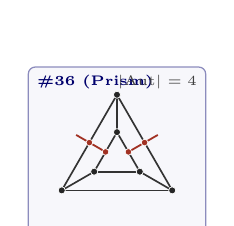
\begin{tikzpicture}[scale=0.88, baseline={(0,0)}]
  \draw[rounded corners=2.5pt, draw=NavyBlue!85!black!45, fill=NavyBlue!85!black!3, line width=0.45pt] (-1.28,-1.18) rectangle (1.28,1.26);
  \node[anchor=north west, font=\tiny\bfseries, text=NavyBlue!85!black, inner sep=1.5pt] at (-1.22,1.21) {\#36 (Prism)};
  \node[anchor=north east, font=\tiny, text=black!75, inner sep=1.5pt] at (1.22,1.21) {$|\mathrm{Aut}|=4$};
  \draw[line width=0.6pt, draw=black!80] (0.000,0.320) -- (0.000,0.860);
  \draw[line width=0.6pt, draw=black!80] (0.000,0.320) -- (0.329,-0.250);
  \draw[line width=0.6pt, draw=black!80] (0.000,0.320) -- (-0.329,-0.250);
  \draw[line width=0.6pt, draw=black!80] (0.000,0.860) -- (-0.797,-0.520);
  \draw[line width=0.6pt, draw=black!80] (0.000,0.860) -- (0.797,-0.520);
  \draw[line width=0.6pt, draw=black!80] (0.329,-0.250) -- (-0.329,-0.250);
  \draw[line width=0.6pt, draw=black!80] (0.329,-0.250) -- (0.797,-0.520);
  \draw[line width=0.6pt, draw=black!80] (-0.329,-0.250) -- (-0.797,-0.520);
  \draw[line width=0.6pt, draw=black!80] (-0.797,-0.520) -- (0.797,-0.520);
  \draw[line width=0.65pt, draw=BrickRed!85!black] (0.165,0.035) -- (0.355,0.145);
  \filldraw[fill=BrickRed!85!black, draw=white, line width=0.25pt] (0.165,0.035) circle (1.35pt);
  \draw[line width=0.65pt, draw=BrickRed!85!black] (-0.165,0.035) -- (-0.355,0.145);
  \filldraw[fill=BrickRed!85!black, draw=white, line width=0.25pt] (-0.165,0.035) circle (1.35pt);
  \draw[line width=0.65pt, draw=BrickRed!85!black] (-0.398,0.170) -- (-0.589,0.280);
  \filldraw[fill=BrickRed!85!black, draw=white, line width=0.25pt] (-0.398,0.170) circle (1.35pt);
  \draw[line width=0.65pt, draw=BrickRed!85!black] (0.398,0.170) -- (0.589,0.280);
  \filldraw[fill=BrickRed!85!black, draw=white, line width=0.25pt] (0.398,0.170) circle (1.35pt);
  \filldraw[fill=black!85, draw=white, line width=0.25pt] (0.000,0.320) circle (1.45pt);
  \filldraw[fill=black!85, draw=white, line width=0.25pt] (-0.329,-0.250) circle (1.45pt);
  \filldraw[fill=black!85, draw=white, line width=0.25pt] (0.329,-0.250) circle (1.45pt);
  \filldraw[fill=black!85, draw=white, line width=0.25pt] (0.000,0.860) circle (1.45pt);
  \filldraw[fill=black!85, draw=white, line width=0.25pt] (-0.797,-0.520) circle (1.45pt);
  \filldraw[fill=black!85, draw=white, line width=0.25pt] (0.797,-0.520) circle (1.45pt);
\end{tikzpicture} &
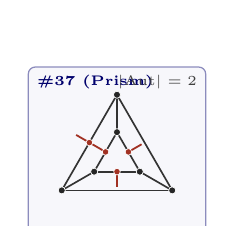
\begin{tikzpicture}[scale=0.88, baseline={(0,0)}]
  \draw[rounded corners=2.5pt, draw=NavyBlue!85!black!45, fill=NavyBlue!85!black!3, line width=0.45pt] (-1.28,-1.18) rectangle (1.28,1.26);
  \node[anchor=north west, font=\tiny\bfseries, text=NavyBlue!85!black, inner sep=1.5pt] at (-1.22,1.21) {\#37 (Prism)};
  \node[anchor=north east, font=\tiny, text=black!75, inner sep=1.5pt] at (1.22,1.21) {$|\mathrm{Aut}|=2$};
  \draw[line width=0.6pt, draw=black!80] (0.000,0.320) -- (0.000,0.860);
  \draw[line width=0.6pt, draw=black!80] (0.000,0.320) -- (0.329,-0.250);
  \draw[line width=0.6pt, draw=black!80] (0.000,0.320) -- (-0.329,-0.250);
  \draw[line width=0.6pt, draw=black!80] (0.000,0.860) -- (-0.797,-0.520);
  \draw[line width=0.6pt, draw=black!80] (0.000,0.860) -- (0.797,-0.520);
  \draw[line width=0.6pt, draw=black!80] (0.329,-0.250) -- (-0.329,-0.250);
  \draw[line width=0.6pt, draw=black!80] (0.329,-0.250) -- (0.797,-0.520);
  \draw[line width=0.6pt, draw=black!80] (-0.329,-0.250) -- (-0.797,-0.520);
  \draw[line width=0.6pt, draw=black!80] (-0.797,-0.520) -- (0.797,-0.520);
  \draw[line width=0.65pt, draw=BrickRed!85!black] (0.165,0.035) -- (0.355,0.145);
  \filldraw[fill=BrickRed!85!black, draw=white, line width=0.25pt] (0.165,0.035) circle (1.35pt);
  \draw[line width=0.65pt, draw=BrickRed!85!black] (-0.165,0.035) -- (-0.355,0.145);
  \filldraw[fill=BrickRed!85!black, draw=white, line width=0.25pt] (-0.165,0.035) circle (1.35pt);
  \draw[line width=0.65pt, draw=BrickRed!85!black] (-0.398,0.170) -- (-0.589,0.280);
  \filldraw[fill=BrickRed!85!black, draw=white, line width=0.25pt] (-0.398,0.170) circle (1.35pt);
  \draw[line width=0.65pt, draw=BrickRed!85!black] (0.000,-0.250) -- (-0.000,-0.470);
  \filldraw[fill=BrickRed!85!black, draw=white, line width=0.25pt] (0.000,-0.250) circle (1.35pt);
  \filldraw[fill=black!85, draw=white, line width=0.25pt] (0.000,0.320) circle (1.45pt);
  \filldraw[fill=black!85, draw=white, line width=0.25pt] (-0.329,-0.250) circle (1.45pt);
  \filldraw[fill=black!85, draw=white, line width=0.25pt] (0.329,-0.250) circle (1.45pt);
  \filldraw[fill=black!85, draw=white, line width=0.25pt] (0.000,0.860) circle (1.45pt);
  \filldraw[fill=black!85, draw=white, line width=0.25pt] (-0.797,-0.520) circle (1.45pt);
  \filldraw[fill=black!85, draw=white, line width=0.25pt] (0.797,-0.520) circle (1.45pt);
\end{tikzpicture} &
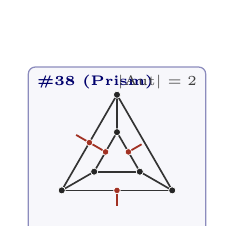
\begin{tikzpicture}[scale=0.88, baseline={(0,0)}]
  \draw[rounded corners=2.5pt, draw=NavyBlue!85!black!45, fill=NavyBlue!85!black!3, line width=0.45pt] (-1.28,-1.18) rectangle (1.28,1.26);
  \node[anchor=north west, font=\tiny\bfseries, text=NavyBlue!85!black, inner sep=1.5pt] at (-1.22,1.21) {\#38 (Prism)};
  \node[anchor=north east, font=\tiny, text=black!75, inner sep=1.5pt] at (1.22,1.21) {$|\mathrm{Aut}|=2$};
  \draw[line width=0.6pt, draw=black!80] (0.000,0.320) -- (0.000,0.860);
  \draw[line width=0.6pt, draw=black!80] (0.000,0.320) -- (0.329,-0.250);
  \draw[line width=0.6pt, draw=black!80] (0.000,0.320) -- (-0.329,-0.250);
  \draw[line width=0.6pt, draw=black!80] (0.000,0.860) -- (-0.797,-0.520);
  \draw[line width=0.6pt, draw=black!80] (0.000,0.860) -- (0.797,-0.520);
  \draw[line width=0.6pt, draw=black!80] (0.329,-0.250) -- (-0.329,-0.250);
  \draw[line width=0.6pt, draw=black!80] (0.329,-0.250) -- (0.797,-0.520);
  \draw[line width=0.6pt, draw=black!80] (-0.329,-0.250) -- (-0.797,-0.520);
  \draw[line width=0.6pt, draw=black!80] (-0.797,-0.520) -- (0.797,-0.520);
  \draw[line width=0.65pt, draw=BrickRed!85!black] (0.165,0.035) -- (0.355,0.145);
  \filldraw[fill=BrickRed!85!black, draw=white, line width=0.25pt] (0.165,0.035) circle (1.35pt);
  \draw[line width=0.65pt, draw=BrickRed!85!black] (-0.165,0.035) -- (-0.355,0.145);
  \filldraw[fill=BrickRed!85!black, draw=white, line width=0.25pt] (-0.165,0.035) circle (1.35pt);
  \draw[line width=0.65pt, draw=BrickRed!85!black] (-0.398,0.170) -- (-0.589,0.280);
  \filldraw[fill=BrickRed!85!black, draw=white, line width=0.25pt] (-0.398,0.170) circle (1.35pt);
  \draw[line width=0.65pt, draw=BrickRed!85!black] (-0.000,-0.520) -- (-0.000,-0.740);
  \filldraw[fill=BrickRed!85!black, draw=white, line width=0.25pt] (-0.000,-0.520) circle (1.35pt);
  \filldraw[fill=black!85, draw=white, line width=0.25pt] (0.000,0.320) circle (1.45pt);
  \filldraw[fill=black!85, draw=white, line width=0.25pt] (-0.329,-0.250) circle (1.45pt);
  \filldraw[fill=black!85, draw=white, line width=0.25pt] (0.329,-0.250) circle (1.45pt);
  \filldraw[fill=black!85, draw=white, line width=0.25pt] (0.000,0.860) circle (1.45pt);
  \filldraw[fill=black!85, draw=white, line width=0.25pt] (-0.797,-0.520) circle (1.45pt);
  \filldraw[fill=black!85, draw=white, line width=0.25pt] (0.797,-0.520) circle (1.45pt);
\end{tikzpicture} &
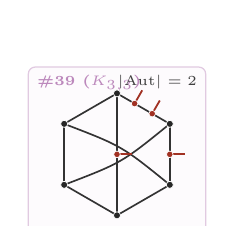
\begin{tikzpicture}[scale=0.88, baseline={(0,0)}]
  \draw[rounded corners=2.5pt, draw=Plum!85!black!45, fill=Plum!85!black!3, line width=0.45pt] (-1.28,-1.18) rectangle (1.28,1.26);
  \node[anchor=north west, font=\tiny\bfseries, text=Plum!85!black, inner sep=1.5pt] at (-1.22,1.21) {\#39 ($K_{3,3}$)};
  \node[anchor=north east, font=\tiny, text=black!75, inner sep=1.5pt] at (1.22,1.21) {$|\mathrm{Aut}|=2$};
  \draw[line width=0.6pt, draw=black!80] (0.000,0.880) -- (0.762,0.440);
  \draw[line width=0.6pt, draw=black!80] (0.000,0.880) -- (0.000,-0.880);
  \draw[line width=0.6pt, draw=black!80] (0.000,0.880) -- (-0.762,0.440);
  \draw[line width=0.6pt, draw=black!80] (0.762,0.440) -- (0.762,-0.440);
  \draw[line width=0.6pt, draw=black!80] (0.762,0.440) .. controls (0.070,-0.121) .. (-0.762,-0.440);
  \draw[line width=0.6pt, draw=black!80] (0.762,-0.440) -- (0.000,-0.880);
  \draw[line width=0.6pt, draw=black!80] (0.762,-0.440) .. controls (0.070,0.121) .. (-0.762,0.440);
  \draw[line width=0.6pt, draw=black!80] (0.000,-0.880) -- (-0.762,-0.440);
  \draw[line width=0.6pt, draw=black!80] (-0.762,-0.440) -- (-0.762,0.440);
  \draw[line width=0.65pt, draw=BrickRed!85!black] (0.254,0.733) -- (0.364,0.924);
  \filldraw[fill=BrickRed!85!black, draw=white, line width=0.25pt] (0.254,0.733) circle (1.35pt);
  \draw[line width=0.65pt, draw=BrickRed!85!black] (0.508,0.587) -- (0.618,0.777);
  \filldraw[fill=BrickRed!85!black, draw=white, line width=0.25pt] (0.508,0.587) circle (1.35pt);
  \draw[line width=0.65pt, draw=BrickRed!85!black] (0.000,0.000) -- (0.220,0.000);
  \filldraw[fill=BrickRed!85!black, draw=white, line width=0.25pt] (0.000,0.000) circle (1.35pt);
  \draw[line width=0.65pt, draw=BrickRed!85!black] (0.762,0.000) -- (0.982,0.000);
  \filldraw[fill=BrickRed!85!black, draw=white, line width=0.25pt] (0.762,0.000) circle (1.35pt);
  \filldraw[fill=black!85, draw=white, line width=0.25pt] (0.000,0.880) circle (1.45pt);
  \filldraw[fill=black!85, draw=white, line width=0.25pt] (0.762,0.440) circle (1.45pt);
  \filldraw[fill=black!85, draw=white, line width=0.25pt] (0.762,-0.440) circle (1.45pt);
  \filldraw[fill=black!85, draw=white, line width=0.25pt] (0.000,-0.880) circle (1.45pt);
  \filldraw[fill=black!85, draw=white, line width=0.25pt] (-0.762,-0.440) circle (1.45pt);
  \filldraw[fill=black!85, draw=white, line width=0.25pt] (-0.762,0.440) circle (1.45pt);
\end{tikzpicture} \\[2pt]
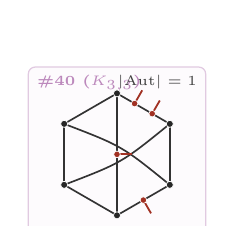
\begin{tikzpicture}[scale=0.88, baseline={(0,0)}]
  \draw[rounded corners=2.5pt, draw=Plum!85!black!45, fill=Plum!85!black!3, line width=0.45pt] (-1.28,-1.18) rectangle (1.28,1.26);
  \node[anchor=north west, font=\tiny\bfseries, text=Plum!85!black, inner sep=1.5pt] at (-1.22,1.21) {\#40 ($K_{3,3}$)};
  \node[anchor=north east, font=\tiny, text=black!75, inner sep=1.5pt] at (1.22,1.21) {$|\mathrm{Aut}|=1$};
  \draw[line width=0.6pt, draw=black!80] (0.000,0.880) -- (0.762,0.440);
  \draw[line width=0.6pt, draw=black!80] (0.000,0.880) -- (0.000,-0.880);
  \draw[line width=0.6pt, draw=black!80] (0.000,0.880) -- (-0.762,0.440);
  \draw[line width=0.6pt, draw=black!80] (0.762,0.440) -- (0.762,-0.440);
  \draw[line width=0.6pt, draw=black!80] (0.762,0.440) .. controls (0.070,-0.121) .. (-0.762,-0.440);
  \draw[line width=0.6pt, draw=black!80] (0.762,-0.440) -- (0.000,-0.880);
  \draw[line width=0.6pt, draw=black!80] (0.762,-0.440) .. controls (0.070,0.121) .. (-0.762,0.440);
  \draw[line width=0.6pt, draw=black!80] (0.000,-0.880) -- (-0.762,-0.440);
  \draw[line width=0.6pt, draw=black!80] (-0.762,-0.440) -- (-0.762,0.440);
  \draw[line width=0.65pt, draw=BrickRed!85!black] (0.254,0.733) -- (0.364,0.924);
  \filldraw[fill=BrickRed!85!black, draw=white, line width=0.25pt] (0.254,0.733) circle (1.35pt);
  \draw[line width=0.65pt, draw=BrickRed!85!black] (0.508,0.587) -- (0.618,0.777);
  \filldraw[fill=BrickRed!85!black, draw=white, line width=0.25pt] (0.508,0.587) circle (1.35pt);
  \draw[line width=0.65pt, draw=BrickRed!85!black] (0.000,0.000) -- (0.220,0.000);
  \filldraw[fill=BrickRed!85!black, draw=white, line width=0.25pt] (0.000,0.000) circle (1.35pt);
  \draw[line width=0.65pt, draw=BrickRed!85!black] (0.381,-0.660) -- (0.491,-0.851);
  \filldraw[fill=BrickRed!85!black, draw=white, line width=0.25pt] (0.381,-0.660) circle (1.35pt);
  \filldraw[fill=black!85, draw=white, line width=0.25pt] (0.000,0.880) circle (1.45pt);
  \filldraw[fill=black!85, draw=white, line width=0.25pt] (0.762,0.440) circle (1.45pt);
  \filldraw[fill=black!85, draw=white, line width=0.25pt] (0.762,-0.440) circle (1.45pt);
  \filldraw[fill=black!85, draw=white, line width=0.25pt] (0.000,-0.880) circle (1.45pt);
  \filldraw[fill=black!85, draw=white, line width=0.25pt] (-0.762,-0.440) circle (1.45pt);
  \filldraw[fill=black!85, draw=white, line width=0.25pt] (-0.762,0.440) circle (1.45pt);
\end{tikzpicture} &
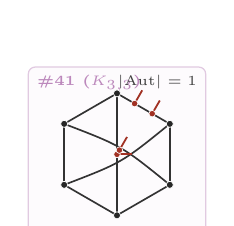
\begin{tikzpicture}[scale=0.88, baseline={(0,0)}]
  \draw[rounded corners=2.5pt, draw=Plum!85!black!45, fill=Plum!85!black!3, line width=0.45pt] (-1.28,-1.18) rectangle (1.28,1.26);
  \node[anchor=north west, font=\tiny\bfseries, text=Plum!85!black, inner sep=1.5pt] at (-1.22,1.21) {\#41 ($K_{3,3}$)};
  \node[anchor=north east, font=\tiny, text=black!75, inner sep=1.5pt] at (1.22,1.21) {$|\mathrm{Aut}|=1$};
  \draw[line width=0.6pt, draw=black!80] (0.000,0.880) -- (0.762,0.440);
  \draw[line width=0.6pt, draw=black!80] (0.000,0.880) -- (0.000,-0.880);
  \draw[line width=0.6pt, draw=black!80] (0.000,0.880) -- (-0.762,0.440);
  \draw[line width=0.6pt, draw=black!80] (0.762,0.440) -- (0.762,-0.440);
  \draw[line width=0.6pt, draw=black!80] (0.762,0.440) .. controls (0.070,-0.121) .. (-0.762,-0.440);
  \draw[line width=0.6pt, draw=black!80] (0.762,-0.440) -- (0.000,-0.880);
  \draw[line width=0.6pt, draw=black!80] (0.762,-0.440) .. controls (0.070,0.121) .. (-0.762,0.440);
  \draw[line width=0.6pt, draw=black!80] (0.000,-0.880) -- (-0.762,-0.440);
  \draw[line width=0.6pt, draw=black!80] (-0.762,-0.440) -- (-0.762,0.440);
  \draw[line width=0.65pt, draw=BrickRed!85!black] (0.254,0.733) -- (0.364,0.924);
  \filldraw[fill=BrickRed!85!black, draw=white, line width=0.25pt] (0.254,0.733) circle (1.35pt);
  \draw[line width=0.65pt, draw=BrickRed!85!black] (0.508,0.587) -- (0.618,0.777);
  \filldraw[fill=BrickRed!85!black, draw=white, line width=0.25pt] (0.508,0.587) circle (1.35pt);
  \draw[line width=0.65pt, draw=BrickRed!85!black] (0.000,0.000) -- (0.220,0.000);
  \filldraw[fill=BrickRed!85!black, draw=white, line width=0.25pt] (0.000,0.000) circle (1.35pt);
  \draw[line width=0.65pt, draw=BrickRed!85!black] (0.035,0.061) -- (0.145,0.251);
  \filldraw[fill=BrickRed!85!black, draw=white, line width=0.25pt] (0.035,0.061) circle (1.35pt);
  \filldraw[fill=black!85, draw=white, line width=0.25pt] (0.000,0.880) circle (1.45pt);
  \filldraw[fill=black!85, draw=white, line width=0.25pt] (0.762,0.440) circle (1.45pt);
  \filldraw[fill=black!85, draw=white, line width=0.25pt] (0.762,-0.440) circle (1.45pt);
  \filldraw[fill=black!85, draw=white, line width=0.25pt] (0.000,-0.880) circle (1.45pt);
  \filldraw[fill=black!85, draw=white, line width=0.25pt] (-0.762,-0.440) circle (1.45pt);
  \filldraw[fill=black!85, draw=white, line width=0.25pt] (-0.762,0.440) circle (1.45pt);
\end{tikzpicture} &
\begin{tikzpicture}[scale=0.88, baseline={(0,0)}]
  \draw[rounded corners=2.5pt, draw=Plum!85!black!45, fill=Plum!85!black!3, line width=0.45pt] (-1.28,-1.18) rectangle (1.28,1.26);
  \node[anchor=north west, font=\tiny\bfseries, text=Plum!85!black, inner sep=1.5pt] at (-1.22,1.21) {\#42 ($K_{3,3}$)};
  \node[anchor=north east, font=\tiny, text=black!75, inner sep=1.5pt] at (1.22,1.21) {$|\mathrm{Aut}|=4$};
  \draw[line width=0.6pt, draw=black!80] (0.000,0.880) -- (0.762,0.440);
  \draw[line width=0.6pt, draw=black!80] (0.000,0.880) -- (0.000,-0.880);
  \draw[line width=0.6pt, draw=black!80] (0.000,0.880) -- (-0.762,0.440);
  \draw[line width=0.6pt, draw=black!80] (0.762,0.440) -- (0.762,-0.440);
  \draw[line width=0.6pt, draw=black!80] (0.762,0.440) .. controls (0.070,-0.121) .. (-0.762,-0.440);
  \draw[line width=0.6pt, draw=black!80] (0.762,-0.440) -- (0.000,-0.880);
  \draw[line width=0.6pt, draw=black!80] (0.762,-0.440) .. controls (0.070,0.121) .. (-0.762,0.440);
  \draw[line width=0.6pt, draw=black!80] (0.000,-0.880) -- (-0.762,-0.440);
  \draw[line width=0.6pt, draw=black!80] (-0.762,-0.440) -- (-0.762,0.440);
  \draw[line width=0.65pt, draw=BrickRed!85!black] (0.254,0.733) -- (0.364,0.924);
  \filldraw[fill=BrickRed!85!black, draw=white, line width=0.25pt] (0.254,0.733) circle (1.35pt);
  \draw[line width=0.65pt, draw=BrickRed!85!black] (0.508,0.587) -- (0.618,0.777);
  \filldraw[fill=BrickRed!85!black, draw=white, line width=0.25pt] (0.508,0.587) circle (1.35pt);
  \draw[line width=0.65pt, draw=BrickRed!85!black] (0.508,-0.587) -- (0.618,-0.777);
  \filldraw[fill=BrickRed!85!black, draw=white, line width=0.25pt] (0.508,-0.587) circle (1.35pt);
  \draw[line width=0.65pt, draw=BrickRed!85!black] (0.254,-0.733) -- (0.364,-0.924);
  \filldraw[fill=BrickRed!85!black, draw=white, line width=0.25pt] (0.254,-0.733) circle (1.35pt);
  \filldraw[fill=black!85, draw=white, line width=0.25pt] (0.000,0.880) circle (1.45pt);
  \filldraw[fill=black!85, draw=white, line width=0.25pt] (0.762,0.440) circle (1.45pt);
  \filldraw[fill=black!85, draw=white, line width=0.25pt] (0.762,-0.440) circle (1.45pt);
  \filldraw[fill=black!85, draw=white, line width=0.25pt] (0.000,-0.880) circle (1.45pt);
  \filldraw[fill=black!85, draw=white, line width=0.25pt] (-0.762,-0.440) circle (1.45pt);
  \filldraw[fill=black!85, draw=white, line width=0.25pt] (-0.762,0.440) circle (1.45pt);
\end{tikzpicture} &
\begin{tikzpicture}[scale=0.88, baseline={(0,0)}]
  \draw[rounded corners=2.5pt, draw=Plum!85!black!45, fill=Plum!85!black!3, line width=0.45pt] (-1.28,-1.18) rectangle (1.28,1.26);
  \node[anchor=north west, font=\tiny\bfseries, text=Plum!85!black, inner sep=1.5pt] at (-1.22,1.21) {\#43 ($K_{3,3}$)};
  \node[anchor=north east, font=\tiny, text=black!75, inner sep=1.5pt] at (1.22,1.21) {$|\mathrm{Aut}|=2$};
  \draw[line width=0.6pt, draw=black!80] (0.000,0.880) -- (0.762,0.440);
  \draw[line width=0.6pt, draw=black!80] (0.000,0.880) -- (0.000,-0.880);
  \draw[line width=0.6pt, draw=black!80] (0.000,0.880) -- (-0.762,0.440);
  \draw[line width=0.6pt, draw=black!80] (0.762,0.440) -- (0.762,-0.440);
  \draw[line width=0.6pt, draw=black!80] (0.762,0.440) .. controls (0.070,-0.121) .. (-0.762,-0.440);
  \draw[line width=0.6pt, draw=black!80] (0.762,-0.440) -- (0.000,-0.880);
  \draw[line width=0.6pt, draw=black!80] (0.762,-0.440) .. controls (0.070,0.121) .. (-0.762,0.440);
  \draw[line width=0.6pt, draw=black!80] (0.000,-0.880) -- (-0.762,-0.440);
  \draw[line width=0.6pt, draw=black!80] (-0.762,-0.440) -- (-0.762,0.440);
  \draw[line width=0.65pt, draw=BrickRed!85!black] (0.254,0.733) -- (0.364,0.924);
  \filldraw[fill=BrickRed!85!black, draw=white, line width=0.25pt] (0.254,0.733) circle (1.35pt);
  \draw[line width=0.65pt, draw=BrickRed!85!black] (0.508,0.587) -- (0.618,0.777);
  \filldraw[fill=BrickRed!85!black, draw=white, line width=0.25pt] (0.508,0.587) circle (1.35pt);
  \draw[line width=0.65pt, draw=BrickRed!85!black] (0.381,-0.660) -- (0.491,-0.851);
  \filldraw[fill=BrickRed!85!black, draw=white, line width=0.25pt] (0.381,-0.660) circle (1.35pt);
  \draw[line width=0.65pt, draw=BrickRed!85!black] (0.035,0.061) -- (0.145,0.251);
  \filldraw[fill=BrickRed!85!black, draw=white, line width=0.25pt] (0.035,0.061) circle (1.35pt);
  \filldraw[fill=black!85, draw=white, line width=0.25pt] (0.000,0.880) circle (1.45pt);
  \filldraw[fill=black!85, draw=white, line width=0.25pt] (0.762,0.440) circle (1.45pt);
  \filldraw[fill=black!85, draw=white, line width=0.25pt] (0.762,-0.440) circle (1.45pt);
  \filldraw[fill=black!85, draw=white, line width=0.25pt] (0.000,-0.880) circle (1.45pt);
  \filldraw[fill=black!85, draw=white, line width=0.25pt] (-0.762,-0.440) circle (1.45pt);
  \filldraw[fill=black!85, draw=white, line width=0.25pt] (-0.762,0.440) circle (1.45pt);
\end{tikzpicture} &
\begin{tikzpicture}[scale=0.88, baseline={(0,0)}]
  \draw[rounded corners=2.5pt, draw=Plum!85!black!45, fill=Plum!85!black!3, line width=0.45pt] (-1.28,-1.18) rectangle (1.28,1.26);
  \node[anchor=north west, font=\tiny\bfseries, text=Plum!85!black, inner sep=1.5pt] at (-1.22,1.21) {\#44 ($K_{3,3}$)};
  \node[anchor=north east, font=\tiny, text=black!75, inner sep=1.5pt] at (1.22,1.21) {$|\mathrm{Aut}|=4$};
  \draw[line width=0.6pt, draw=black!80] (0.000,0.880) -- (0.762,0.440);
  \draw[line width=0.6pt, draw=black!80] (0.000,0.880) -- (0.000,-0.880);
  \draw[line width=0.6pt, draw=black!80] (0.000,0.880) -- (-0.762,0.440);
  \draw[line width=0.6pt, draw=black!80] (0.762,0.440) -- (0.762,-0.440);
  \draw[line width=0.6pt, draw=black!80] (0.762,0.440) .. controls (0.070,-0.121) .. (-0.762,-0.440);
  \draw[line width=0.6pt, draw=black!80] (0.762,-0.440) -- (0.000,-0.880);
  \draw[line width=0.6pt, draw=black!80] (0.762,-0.440) .. controls (0.070,0.121) .. (-0.762,0.440);
  \draw[line width=0.6pt, draw=black!80] (0.000,-0.880) -- (-0.762,-0.440);
  \draw[line width=0.6pt, draw=black!80] (-0.762,-0.440) -- (-0.762,0.440);
  \draw[line width=0.65pt, draw=BrickRed!85!black] (0.254,0.733) -- (0.364,0.924);
  \filldraw[fill=BrickRed!85!black, draw=white, line width=0.25pt] (0.254,0.733) circle (1.35pt);
  \draw[line width=0.65pt, draw=BrickRed!85!black] (0.508,0.587) -- (0.618,0.777);
  \filldraw[fill=BrickRed!85!black, draw=white, line width=0.25pt] (0.508,0.587) circle (1.35pt);
  \draw[line width=0.65pt, draw=BrickRed!85!black] (0.381,-0.660) -- (0.491,-0.851);
  \filldraw[fill=BrickRed!85!black, draw=white, line width=0.25pt] (0.381,-0.660) circle (1.35pt);
  \draw[line width=0.65pt, draw=BrickRed!85!black] (-0.762,0.000) -- (-0.982,0.000);
  \filldraw[fill=BrickRed!85!black, draw=white, line width=0.25pt] (-0.762,0.000) circle (1.35pt);
  \filldraw[fill=black!85, draw=white, line width=0.25pt] (0.000,0.880) circle (1.45pt);
  \filldraw[fill=black!85, draw=white, line width=0.25pt] (0.762,0.440) circle (1.45pt);
  \filldraw[fill=black!85, draw=white, line width=0.25pt] (0.762,-0.440) circle (1.45pt);
  \filldraw[fill=black!85, draw=white, line width=0.25pt] (0.000,-0.880) circle (1.45pt);
  \filldraw[fill=black!85, draw=white, line width=0.25pt] (-0.762,-0.440) circle (1.45pt);
  \filldraw[fill=black!85, draw=white, line width=0.25pt] (-0.762,0.440) circle (1.45pt);
\end{tikzpicture} \\[2pt]
\begin{tikzpicture}[scale=0.88, baseline={(0,0)}]
  \draw[rounded corners=2.5pt, draw=Plum!85!black!45, fill=Plum!85!black!3, line width=0.45pt] (-1.28,-1.18) rectangle (1.28,1.26);
  \node[anchor=north west, font=\tiny\bfseries, text=Plum!85!black, inner sep=1.5pt] at (-1.22,1.21) {\#45 ($K_{3,3}$)};
  \node[anchor=north east, font=\tiny, text=black!75, inner sep=1.5pt] at (1.22,1.21) {$|\mathrm{Aut}|=2$};
  \draw[line width=0.6pt, draw=black!80] (0.000,0.880) -- (0.762,0.440);
  \draw[line width=0.6pt, draw=black!80] (0.000,0.880) -- (0.000,-0.880);
  \draw[line width=0.6pt, draw=black!80] (0.000,0.880) -- (-0.762,0.440);
  \draw[line width=0.6pt, draw=black!80] (0.762,0.440) -- (0.762,-0.440);
  \draw[line width=0.6pt, draw=black!80] (0.762,0.440) .. controls (0.070,-0.121) .. (-0.762,-0.440);
  \draw[line width=0.6pt, draw=black!80] (0.762,-0.440) -- (0.000,-0.880);
  \draw[line width=0.6pt, draw=black!80] (0.762,-0.440) .. controls (0.070,0.121) .. (-0.762,0.440);
  \draw[line width=0.6pt, draw=black!80] (0.000,-0.880) -- (-0.762,-0.440);
  \draw[line width=0.6pt, draw=black!80] (-0.762,-0.440) -- (-0.762,0.440);
  \draw[line width=0.65pt, draw=BrickRed!85!black] (0.381,0.660) -- (0.491,0.851);
  \filldraw[fill=BrickRed!85!black, draw=white, line width=0.25pt] (0.381,0.660) circle (1.35pt);
  \draw[line width=0.65pt, draw=BrickRed!85!black] (0.000,0.000) -- (0.220,0.000);
  \filldraw[fill=BrickRed!85!black, draw=white, line width=0.25pt] (0.000,0.000) circle (1.35pt);
  \draw[line width=0.65pt, draw=BrickRed!85!black] (-0.381,0.660) -- (-0.491,0.851);
  \filldraw[fill=BrickRed!85!black, draw=white, line width=0.25pt] (-0.381,0.660) circle (1.35pt);
  \draw[line width=0.65pt, draw=BrickRed!85!black] (0.762,0.000) -- (0.982,0.000);
  \filldraw[fill=BrickRed!85!black, draw=white, line width=0.25pt] (0.762,0.000) circle (1.35pt);
  \filldraw[fill=black!85, draw=white, line width=0.25pt] (0.000,0.880) circle (1.45pt);
  \filldraw[fill=black!85, draw=white, line width=0.25pt] (0.762,0.440) circle (1.45pt);
  \filldraw[fill=black!85, draw=white, line width=0.25pt] (0.762,-0.440) circle (1.45pt);
  \filldraw[fill=black!85, draw=white, line width=0.25pt] (0.000,-0.880) circle (1.45pt);
  \filldraw[fill=black!85, draw=white, line width=0.25pt] (-0.762,-0.440) circle (1.45pt);
  \filldraw[fill=black!85, draw=white, line width=0.25pt] (-0.762,0.440) circle (1.45pt);
\end{tikzpicture} &
\begin{tikzpicture}[scale=0.88, baseline={(0,0)}]
  \draw[rounded corners=2.5pt, draw=Plum!85!black!45, fill=Plum!85!black!3, line width=0.45pt] (-1.28,-1.18) rectangle (1.28,1.26);
  \node[anchor=north west, font=\tiny\bfseries, text=Plum!85!black, inner sep=1.5pt] at (-1.22,1.21) {\#46 ($K_{3,3}$)};
  \node[anchor=north east, font=\tiny, text=black!75, inner sep=1.5pt] at (1.22,1.21) {$|\mathrm{Aut}|=8$};
  \draw[line width=0.6pt, draw=black!80] (0.000,0.880) -- (0.762,0.440);
  \draw[line width=0.6pt, draw=black!80] (0.000,0.880) -- (0.000,-0.880);
  \draw[line width=0.6pt, draw=black!80] (0.000,0.880) -- (-0.762,0.440);
  \draw[line width=0.6pt, draw=black!80] (0.762,0.440) -- (0.762,-0.440);
  \draw[line width=0.6pt, draw=black!80] (0.762,0.440) .. controls (0.070,-0.121) .. (-0.762,-0.440);
  \draw[line width=0.6pt, draw=black!80] (0.762,-0.440) -- (0.000,-0.880);
  \draw[line width=0.6pt, draw=black!80] (0.762,-0.440) .. controls (0.070,0.121) .. (-0.762,0.440);
  \draw[line width=0.6pt, draw=black!80] (0.000,-0.880) -- (-0.762,-0.440);
  \draw[line width=0.6pt, draw=black!80] (-0.762,-0.440) -- (-0.762,0.440);
  \draw[line width=0.65pt, draw=BrickRed!85!black] (0.381,0.660) -- (0.491,0.851);
  \filldraw[fill=BrickRed!85!black, draw=white, line width=0.25pt] (0.381,0.660) circle (1.35pt);
  \draw[line width=0.65pt, draw=BrickRed!85!black] (0.000,0.000) -- (0.220,0.000);
  \filldraw[fill=BrickRed!85!black, draw=white, line width=0.25pt] (0.000,0.000) circle (1.35pt);
  \draw[line width=0.65pt, draw=BrickRed!85!black] (0.762,0.000) -- (0.982,0.000);
  \filldraw[fill=BrickRed!85!black, draw=white, line width=0.25pt] (0.762,0.000) circle (1.35pt);
  \draw[line width=0.65pt, draw=BrickRed!85!black] (0.381,-0.660) -- (0.491,-0.851);
  \filldraw[fill=BrickRed!85!black, draw=white, line width=0.25pt] (0.381,-0.660) circle (1.35pt);
  \filldraw[fill=black!85, draw=white, line width=0.25pt] (0.000,0.880) circle (1.45pt);
  \filldraw[fill=black!85, draw=white, line width=0.25pt] (0.762,0.440) circle (1.45pt);
  \filldraw[fill=black!85, draw=white, line width=0.25pt] (0.762,-0.440) circle (1.45pt);
  \filldraw[fill=black!85, draw=white, line width=0.25pt] (0.000,-0.880) circle (1.45pt);
  \filldraw[fill=black!85, draw=white, line width=0.25pt] (-0.762,-0.440) circle (1.45pt);
  \filldraw[fill=black!85, draw=white, line width=0.25pt] (-0.762,0.440) circle (1.45pt);
\end{tikzpicture} &
\begin{tikzpicture}[scale=0.88, baseline={(0,0)}]
  \draw[rounded corners=2.5pt, draw=Plum!85!black!45, fill=Plum!85!black!3, line width=0.45pt] (-1.28,-1.18) rectangle (1.28,1.26);
  \node[anchor=north west, font=\tiny\bfseries, text=Plum!85!black, inner sep=1.5pt] at (-1.22,1.21) {\#47 ($K_{3,3}$)};
  \node[anchor=north east, font=\tiny, text=black!75, inner sep=1.5pt] at (1.22,1.21) {$|\mathrm{Aut}|=2$};
  \draw[line width=0.6pt, draw=black!80] (0.000,0.880) -- (0.762,0.440);
  \draw[line width=0.6pt, draw=black!80] (0.000,0.880) -- (0.000,-0.880);
  \draw[line width=0.6pt, draw=black!80] (0.000,0.880) -- (-0.762,0.440);
  \draw[line width=0.6pt, draw=black!80] (0.762,0.440) -- (0.762,-0.440);
  \draw[line width=0.6pt, draw=black!80] (0.762,0.440) .. controls (0.070,-0.121) .. (-0.762,-0.440);
  \draw[line width=0.6pt, draw=black!80] (0.762,-0.440) -- (0.000,-0.880);
  \draw[line width=0.6pt, draw=black!80] (0.762,-0.440) .. controls (0.070,0.121) .. (-0.762,0.440);
  \draw[line width=0.6pt, draw=black!80] (0.000,-0.880) -- (-0.762,-0.440);
  \draw[line width=0.6pt, draw=black!80] (-0.762,-0.440) -- (-0.762,0.440);
  \draw[line width=0.65pt, draw=BrickRed!85!black] (0.381,0.660) -- (0.491,0.851);
  \filldraw[fill=BrickRed!85!black, draw=white, line width=0.25pt] (0.381,0.660) circle (1.35pt);
  \draw[line width=0.65pt, draw=BrickRed!85!black] (0.000,0.000) -- (0.220,0.000);
  \filldraw[fill=BrickRed!85!black, draw=white, line width=0.25pt] (0.000,0.000) circle (1.35pt);
  \draw[line width=0.65pt, draw=BrickRed!85!black] (0.762,0.000) -- (0.982,0.000);
  \filldraw[fill=BrickRed!85!black, draw=white, line width=0.25pt] (0.762,0.000) circle (1.35pt);
  \draw[line width=0.65pt, draw=BrickRed!85!black] (0.035,0.061) -- (0.145,0.251);
  \filldraw[fill=BrickRed!85!black, draw=white, line width=0.25pt] (0.035,0.061) circle (1.35pt);
  \filldraw[fill=black!85, draw=white, line width=0.25pt] (0.000,0.880) circle (1.45pt);
  \filldraw[fill=black!85, draw=white, line width=0.25pt] (0.762,0.440) circle (1.45pt);
  \filldraw[fill=black!85, draw=white, line width=0.25pt] (0.762,-0.440) circle (1.45pt);
  \filldraw[fill=black!85, draw=white, line width=0.25pt] (0.000,-0.880) circle (1.45pt);
  \filldraw[fill=black!85, draw=white, line width=0.25pt] (-0.762,-0.440) circle (1.45pt);
  \filldraw[fill=black!85, draw=white, line width=0.25pt] (-0.762,0.440) circle (1.45pt);
\end{tikzpicture} &
\begin{tikzpicture}[scale=0.88, baseline={(0,0)}]
  \draw[rounded corners=2.5pt, draw=Plum!85!black!45, fill=Plum!85!black!3, line width=0.45pt] (-1.28,-1.18) rectangle (1.28,1.26);
  \node[anchor=north west, font=\tiny\bfseries, text=Plum!85!black, inner sep=1.5pt] at (-1.22,1.21) {\#48 ($K_{3,3}$)};
  \node[anchor=north east, font=\tiny, text=black!75, inner sep=1.5pt] at (1.22,1.21) {$|\mathrm{Aut}|=2$};
  \draw[line width=0.6pt, draw=black!80] (0.000,0.880) -- (0.762,0.440);
  \draw[line width=0.6pt, draw=black!80] (0.000,0.880) -- (0.000,-0.880);
  \draw[line width=0.6pt, draw=black!80] (0.000,0.880) -- (-0.762,0.440);
  \draw[line width=0.6pt, draw=black!80] (0.762,0.440) -- (0.762,-0.440);
  \draw[line width=0.6pt, draw=black!80] (0.762,0.440) .. controls (0.070,-0.121) .. (-0.762,-0.440);
  \draw[line width=0.6pt, draw=black!80] (0.762,-0.440) -- (0.000,-0.880);
  \draw[line width=0.6pt, draw=black!80] (0.762,-0.440) .. controls (0.070,0.121) .. (-0.762,0.440);
  \draw[line width=0.6pt, draw=black!80] (0.000,-0.880) -- (-0.762,-0.440);
  \draw[line width=0.6pt, draw=black!80] (-0.762,-0.440) -- (-0.762,0.440);
  \draw[line width=0.65pt, draw=BrickRed!85!black] (0.381,0.660) -- (0.491,0.851);
  \filldraw[fill=BrickRed!85!black, draw=white, line width=0.25pt] (0.381,0.660) circle (1.35pt);
  \draw[line width=0.65pt, draw=BrickRed!85!black] (0.000,0.000) -- (0.220,0.000);
  \filldraw[fill=BrickRed!85!black, draw=white, line width=0.25pt] (0.000,0.000) circle (1.35pt);
  \draw[line width=0.65pt, draw=BrickRed!85!black] (0.762,0.000) -- (0.982,0.000);
  \filldraw[fill=BrickRed!85!black, draw=white, line width=0.25pt] (0.762,0.000) circle (1.35pt);
  \draw[line width=0.65pt, draw=BrickRed!85!black] (-0.762,0.000) -- (-0.982,0.000);
  \filldraw[fill=BrickRed!85!black, draw=white, line width=0.25pt] (-0.762,0.000) circle (1.35pt);
  \filldraw[fill=black!85, draw=white, line width=0.25pt] (0.000,0.880) circle (1.45pt);
  \filldraw[fill=black!85, draw=white, line width=0.25pt] (0.762,0.440) circle (1.45pt);
  \filldraw[fill=black!85, draw=white, line width=0.25pt] (0.762,-0.440) circle (1.45pt);
  \filldraw[fill=black!85, draw=white, line width=0.25pt] (0.000,-0.880) circle (1.45pt);
  \filldraw[fill=black!85, draw=white, line width=0.25pt] (-0.762,-0.440) circle (1.45pt);
  \filldraw[fill=black!85, draw=white, line width=0.25pt] (-0.762,0.440) circle (1.45pt);
\end{tikzpicture} &
\begin{tikzpicture}[scale=0.88, baseline={(0,0)}]
  \draw[rounded corners=2.5pt, draw=Plum!85!black!45, fill=Plum!85!black!3, line width=0.45pt] (-1.28,-1.18) rectangle (1.28,1.26);
  \node[anchor=north west, font=\tiny\bfseries, text=Plum!85!black, inner sep=1.5pt] at (-1.22,1.21) {\#49 ($K_{3,3}$)};
  \node[anchor=north east, font=\tiny, text=black!75, inner sep=1.5pt] at (1.22,1.21) {$|\mathrm{Aut}|=8$};
  \draw[line width=0.6pt, draw=black!80] (0.000,0.880) -- (0.762,0.440);
  \draw[line width=0.6pt, draw=black!80] (0.000,0.880) -- (0.000,-0.880);
  \draw[line width=0.6pt, draw=black!80] (0.000,0.880) -- (-0.762,0.440);
  \draw[line width=0.6pt, draw=black!80] (0.762,0.440) -- (0.762,-0.440);
  \draw[line width=0.6pt, draw=black!80] (0.762,0.440) .. controls (0.070,-0.121) .. (-0.762,-0.440);
  \draw[line width=0.6pt, draw=black!80] (0.762,-0.440) -- (0.000,-0.880);
  \draw[line width=0.6pt, draw=black!80] (0.762,-0.440) .. controls (0.070,0.121) .. (-0.762,0.440);
  \draw[line width=0.6pt, draw=black!80] (0.000,-0.880) -- (-0.762,-0.440);
  \draw[line width=0.6pt, draw=black!80] (-0.762,-0.440) -- (-0.762,0.440);
  \draw[line width=0.65pt, draw=BrickRed!85!black] (0.381,0.660) -- (0.491,0.851);
  \filldraw[fill=BrickRed!85!black, draw=white, line width=0.25pt] (0.381,0.660) circle (1.35pt);
  \draw[line width=0.65pt, draw=BrickRed!85!black] (0.000,0.000) -- (0.220,0.000);
  \filldraw[fill=BrickRed!85!black, draw=white, line width=0.25pt] (0.000,0.000) circle (1.35pt);
  \draw[line width=0.65pt, draw=BrickRed!85!black] (0.035,0.061) -- (0.145,0.251);
  \filldraw[fill=BrickRed!85!black, draw=white, line width=0.25pt] (0.035,0.061) circle (1.35pt);
  \draw[line width=0.65pt, draw=BrickRed!85!black] (-0.762,0.000) -- (-0.982,0.000);
  \filldraw[fill=BrickRed!85!black, draw=white, line width=0.25pt] (-0.762,0.000) circle (1.35pt);
  \filldraw[fill=black!85, draw=white, line width=0.25pt] (0.000,0.880) circle (1.45pt);
  \filldraw[fill=black!85, draw=white, line width=0.25pt] (0.762,0.440) circle (1.45pt);
  \filldraw[fill=black!85, draw=white, line width=0.25pt] (0.762,-0.440) circle (1.45pt);
  \filldraw[fill=black!85, draw=white, line width=0.25pt] (0.000,-0.880) circle (1.45pt);
  \filldraw[fill=black!85, draw=white, line width=0.25pt] (-0.762,-0.440) circle (1.45pt);
  \filldraw[fill=black!85, draw=white, line width=0.25pt] (-0.762,0.440) circle (1.45pt);
\end{tikzpicture} \\[2pt]
\end{tabular}
\caption{Complete bare four-loop Feynman diagram atlas on $\mathbb{R}\times\mathbb{C}^2$, Part~II: Graphs \texttt{\#25}--\texttt{\#49} (comprising the remaining $14$ triangular-prism topologies \texttt{\#25}--\texttt{\#38} and all $11$ non-planar bipartite $K_{3,3}$ topologies \texttt{\#39}--\texttt{\#49}, where antipodal chords are bowed slightly around the center to keep every crossing legible).}
\label{fig:atlas-25-49}
\end{figure}


\begin{table}[H]
\centering
\scriptsize
\setlength{\tabcolsep}{4.8pt}
\renewcommand{\arraystretch}{1.48}
\begin{tabular}{@{}llccc@{}}
\toprule
\textbf{Core Family \& Indices} & \textbf{Count} & \textbf{Coefficient of $N^0$} & \textbf{Coefficient of $N^2$} & \textbf{Coefficient of $N^4$} \\
\midrule
Core I: Series--Parallel (\texttt{\#00}--\texttt{\#02}) & $3$ & $0$ & $0$ & $+\dfrac{1}{10500}$ \\[4.5pt]
Core III: Doubled-Kite (\texttt{\#03}--\texttt{\#10}) & $8$ & $\dfrac{101}{945} - \dfrac{1241\pi^2}{45360}$ & $\dfrac{73903}{1020600} - \dfrac{37\pi^2}{3402}$ & $\dfrac{34259}{20412000} - \dfrac{11\pi^2}{829440}$ \\[4.5pt]
Core IV: Triangular Prism (\texttt{\#11}--\texttt{\#38}) & $28$ & $\dfrac{9796575\pi^2 - 96791482}{12247200}$ & $\dfrac{88921725\pi^2 - 884922356}{734832000}$ & $\dfrac{144949856 - 14698125\pi^2}{653184000}$ \\[4.5pt]
Core V: Non-Planar $K_{3,3}$ (\texttt{\#39}--\texttt{\#49}) & $11$ & $\dfrac{93253402 - 9461505\pi^2}{12247200}$ & $\dfrac{734213669 - 74453325\pi^2}{183708000}$ & $0$ \\
\midrule
\textbf{Total $50$-Graph Bare Sum} ($/\pi^2$) & $\mathbf{50}$ & $-\dfrac{172}{945}$ & $\dfrac{139229}{48600} - \dfrac{35701\pi^2}{120960}$ & $\dfrac{760981}{3402000} - \dfrac{130727\pi^2}{5806080}$ \\
\bottomrule
\end{tabular}
\caption{Exact cyclic-probe sums (divided by $\pi^2$ prior to the four-loop heat normalization $\frac{1}{(8\pi^{5/2})^4} = \frac{(\epsilon\pi\nu)^2}{\pi^2}$) across the four surviving core families of Figures~\ref{fig:atlas-00-24}--\ref{fig:atlas-25-49}. Notice the exact cancellation of $\pi^2$ in the $N^0$ column across Kite, Prism, and $K_{3,3}$!}
\label{tab:fourloop-core-sums}
\end{table}

\begin{theorem}[Exact fourth-order counterterm]
\label{thm:i4}
In the heat-kernel scheme and Wick convention $\epsilon U = +1$, the unique $\mathrm{U}(2)$-equivariant fourth-order Taylor cochain on $\fsl_N$ ($\kappa = \tr$, valid for both roots $\pm a$ and specializing to every integer $N \ge 2$) is
\begin{equation}
\label{eq:i4-closed}
i_4 = \frac{1}{4096\pi^8}\left[\frac{1}{24} + N^2\left(\frac{1102559}{5443200} - \frac{35701\pi^2}{1935360}\right) + N^4\left(\frac{4216}{212625} - \frac{130727\pi^2}{92897280}\right)\right][p^{(0)}p^{(1)}]^4\tr(X_0[X_1,X_2]).
\end{equation}
\end{theorem}

\begin{proof}
By Theorem~\ref{thm:all-orders-traceless}, closedness and uniqueness hold prior to evaluation, and dividing the total probe value by $16$ extracts $c_4(N)$: adding $\frac{21221N^4 + 85304N^2 + 192480}{3628800}$ (Figure~\ref{fig:fourloop-sp-and-marked}B) to $\frac{1}{16}$ of the total bare row in Table~\ref{tab:fourloop-core-sums} gives~\eqref{eq:i4-closed}, verified independently across all $300$ rational and $300$ $\pi^2$ full-cochain trace--momentum coordinates~\cite[\S6.2]{RepoAllOrders}.
\end{proof}

\begin{corollary}[Positivity and transcendence at every $N \ge 2$]
\label{cor:i4-transcendental}
For every integer $N \ge 2$, the scalar bracket in~\eqref{eq:i4-closed} is strictly positive and transcendental.
\end{corollary}

\begin{proof}
Using $\pi^2 < 10$ gives $\frac{1102559}{5443200} - \frac{35701\pi^2}{1935360} > \frac{787747}{43545600} > 0$ and $\frac{4216}{212625} - \frac{130727\pi^2}{92897280} > \frac{2864617}{497664000} > 0$, while the rational multiplier $-\big(\frac{35701N^2}{1935360} + \frac{130727N^4}{92897280}\big)$ of $\pi^2$ is strictly negative for all $N \ge 2$; Lindemann's transcendence of $\pi$ completes the proof.
\end{proof}

\begin{example}[Worked benchmarks: $N^0\pi^2$ cross-core cancellation, $\frac{1}{24}$ constant term, and $\fsl_2$ specialization]
\label{ex:i4-checks}
Table~\ref{tab:fourloop-core-sums} and Theorem~\ref{thm:i4} exhibit three concrete algebraic specializations:
\begin{enumerate}[label=(\alph*),leftmargin=*]
  \item \textbf{Cross-core $[\pi^2 N^0]$ cancellation and $\frac{1}{24}$ constant term:} Placing the $[\pi^2 N^0]$ coefficients of Kite, Prism, and $K_{3,3}$ over $12247200 = 270 \cdot 45360$ gives $\frac{-270\cdot 1241 + 9796575 - 9461505}{12247200} = \frac{-335070 + 335070}{12247200} = 0$, while the rational $N^0$ pieces combine as $\frac{192480}{3628800} - \frac{172}{16\cdot 945} = \frac{401 - 86}{7560} = \frac{315}{7560} = \frac{1}{24}$.
  \item \textbf{Rank-two specialization $N = 2$ ($\fsl_2$):} Substituting $N^2 = 4$ and $N^4 = 16$ into~\eqref{eq:i4-closed} gives $\frac{1}{24} + \frac{1102559}{1360800} + \frac{67456}{212625} = \frac{2651629}{2268000}$ for the rational piece and $-\frac{35701}{483840} - \frac{130727}{5806080} = -\frac{559139}{5806080} = -\frac{79877}{829440}$ for the $\pi^2$ multiplier, yielding the strictly positive transcendental $\fsl_2$ counterterm $i_4|_{\fsl_2} = \frac{1}{4096\pi^8}\big(\frac{2651629}{2268000} - \frac{79877\pi^2}{829440}\big)[p^{(0)}p^{(1)}]^4 f > 0$ (where all $D$ and $D_3$ vertices vanish identically on $\fsl_2$, leaving $\frac{1}{2}\{I_2,I_2\}$, $1\times I_2$ marked thetas, and the $50$ bare four-loop graphs).
\end{enumerate}
\end{example}

% ============================================================================
\section{Two-Loop Cancellation by a Central Field and M-Theory Bridges}
\label{sec:central-moyal}
% ============================================================================

\subsection{Complete five-sector cancellation on $\fg \oplus \mathbb{C}\mathbf{1}$ ($\fso_5\oplus\mathbb{C}$ and $G_2..E_8$)}
\label{subsec:central-extension}

Semisimplicity in Theorem~\ref{thm:uniform-nogo} and Corollary~\ref{cor:semisimple-class} is indispensable! Physically (Table~\ref{tab:cs-ladder}), adjoining one abelian $\mathrm{U}(1)$ gauge superfield $\mathbf{1}$ to a Killing-normalized simple Lie algebra $\fg$ ($\kappa(X,\mathbf{1}) = 0$, $\kappa(\mathbf{1},\mathbf{1}) = \ell \neq 0$) enables the mixed topological $5\mathrm{D}$ Chern--Simons coupling $A_{\mathbf{1}}\wedge\kappa(F_{\fg}\wedge F_{\fg}) + \frac{\gamma}{3\chi}A_{\mathbf{1}}\wedge F_{\mathbf{1}}^2$, whose HT Taylor cochain is $j(X_0,X_1,X_2) = [p^{(0)}p^{(1)}]T(X_0,X_1,X_2)$ with symmetric tensor
\begin{equation}
\label{eq:central-T-def}
T(X, Y, \mathbf{1}) = \chi\,\kappa(X, Y), \qquad T(\mathbf{1}, \mathbf{1}, \mathbf{1}) = \gamma, \qquad T(X, Y, Z) = 0, \qquad T(X, \mathbf{1}, \mathbf{1}) = 0 \quad (X,Y,Z \in \fg).
\end{equation}
Figure~\ref{fig:central-extension-sectors} displays the tree-level Feynman diagrams generated by $\frac{1}{2}\{j, j\}$ across all five external central-leg sectors $c \in \{0,1,2,3,4\}$.

\begin{figure}[H]
\centering
\begin{tikzpicture}[scale=0.91]
  \draw[rounded corners=3pt, draw=Plum!55, fill=Plum!2, line width=0.5pt] (-8.20,-2.35) rectangle (8.20,2.30);
  \node[font=\scriptsize\bfseries, text=Plum!85!black] at (0,1.96) {Five-Sector Tree Brackets $\frac{1}{2}\{j, j\}$ on $\fg\oplus\mathbb{C}\mathbf{1}$ (Solid $=$ Simple $\fg$, Blue Dashed $=$ Central $\mathbf{1}$)};
  \draw[Plum!35, line width=0.45pt] (-3.15,-2.15) -- (-3.15,1.65);
  \draw[Plum!35, line width=0.45pt] ( 3.35,-2.15) -- ( 3.35,1.65);

  % Sector c=0: central exchange cancels bare theta G_kk!
  \begin{scope}[xshift=-5.68cm, yshift=0.35cm]
    \coordinate (a1) at (-0.52,0); \coordinate (a2) at (0.52,0);
    \draw[cprop] (a1) -- node[above, font=\tiny, text=RoyalBlue!85!black] {$\ell^{-1}$} (a2);
    \draw[prop] (a1) -- ++(-0.44, 0.44) node[left=-1pt, font=\tiny] {$X_0$};
    \draw[prop] (a1) -- ++(-0.44,-0.44) node[left=-1pt, font=\tiny] {$X_1$};
    \draw[prop] (a2) -- ++( 0.44, 0.44) node[right=-1pt, font=\tiny] {$X_2$};
    \draw[prop] (a2) -- ++( 0.44,-0.44) node[right=-1pt, font=\tiny] {$X_3$};
    \node[vtcent] at (a1) {}; \node[vtcent] at (a2) {};
    \node[font=\tiny, align=center] at (0,-1.68) {\textbf{$c = 0$ ($4$ simple legs):}\\[2pt]$+\dfrac{\chi^2}{8\ell}G_{kk}$ (cancels $a_{\mathrm{cent}}G_{kk}$)};
  \end{scope}

  % Sector c=2: s-channel vs t,u-channels -> gamma = ell * chi
  \begin{scope}[xshift=0.10cm, yshift=0.38cm]
    % s-channel
    \coordinate (b1) at (-1.85,0); \coordinate (b2) at (-0.98,0);
    \draw[cprop] (b1) -- node[above, font=\tiny, text=RoyalBlue!85!black] {$\ell^{-1}$} (b2);
    \draw[prop] (b1) -- ++(-0.36, 0.40) node[left=-1pt, font=\tiny] {$X_0$};
    \draw[prop] (b1) -- ++(-0.36,-0.40) node[left=-1pt, font=\tiny] {$X_1$};
    \draw[cextleg] (b2) -- ++( 0.36, 0.40) node[right=-1pt, font=\tiny, text=RoyalBlue!85!black] {$\mathbf{1}$};
    \draw[cextleg] (b2) -- ++( 0.36,-0.40) node[right=-1pt, font=\tiny, text=RoyalBlue!85!black] {$\mathbf{1}$};
    \node[vtcent] at (b1) {}; \node[vtcent] at (b2) {};
    \node[font=\tiny] at (-1.42,-0.78) {$\frac{\chi\gamma}{\ell}[01][23]$};

    \node[font=\scriptsize\bfseries] at (-0.08,0) {$-$};

    % t,u-channels
    \coordinate (c1) at (1.15,0.34); \coordinate (c2) at (1.15,-0.34);
    \draw[prop] (c1) -- node[right=1.5pt, font=\tiny] {$\kappa^{-1}$} (c2);
    \draw[prop] (c1) -- ++(-0.42, 0.22) node[left=-1pt, font=\tiny] {$X_0$};
    \draw[cextleg] (c1) -- ++( 0.42, 0.22) node[right=-1pt, font=\tiny, text=RoyalBlue!85!black] {$\mathbf{1}$};
    \draw[prop] (c2) -- ++(-0.42,-0.22) node[left=-1pt, font=\tiny] {$X_1$};
    \draw[cextleg] (c2) -- ++( 0.42,-0.22) node[right=-1pt, font=\tiny, text=RoyalBlue!85!black] {$\mathbf{1}$};
    \node[vtcent] at (c1) {}; \node[vtcent] at (c2) {};
    \node[font=\tiny] at (1.18,-0.88) {$\chi^2([02][13]{-}[03][12])$};

    \node[font=\tiny, align=center, text=Plum!85!black] at (0,-1.72) {\textbf{$c = 2$ ($2$ simple, $2$ central):} Pl\"ucker $\implies$\\$\chi(\frac{\gamma}{\ell}-\chi)[01][23]\kappa(X_0,X_1) = 0 \iff \mathbf{\gamma = \ell\chi}$};
  \end{scope}

  % Sector c=4 & c=1,3
  \begin{scope}[xshift=5.78cm, yshift=0.35cm]
    \coordinate (d1) at (-0.48,0); \coordinate (d2) at (0.48,0);
    \draw[cprop] (d1) -- (d2);
    \draw[cextleg] (d1) -- ++(-0.40, 0.40); \draw[cextleg] (d1) -- ++(-0.40,-0.40);
    \draw[cextleg] (d2) -- ++( 0.40, 0.40); \draw[cextleg] (d2) -- ++( 0.40,-0.40);
    \node[vtcent] at (d1) {}; \node[vtcent] at (d2) {};
    \node[font=\tiny, align=center] at (0,-1.68) {\textbf{$c = 1, 3, 4$:} vanish identically\\($c=4$ by Pl\"ucker)};
  \end{scope}
\end{tikzpicture}
\caption{Tree-level central-extension diagrams $\frac{1}{2}\{j, j\}$ across all external sectors $c = 0..4$. At $c=0$, exchanging a central $\mathbf{1}$-propagator generates $G_{kk}$ on $\fg^{\otimes 4}$; at $c=2$, cancelling $s$-channel central exchange against $t,u$-channel $\fg$-exchange via Pl\"ucker's identity forces $\gamma = \ell\chi$.}
\label{fig:central-extension-sectors}
\end{figure}

\begin{proposition}[Complete central-field square across all external sectors]
\label{prop:central-square}
The cochain $j = [p^{(0)}p^{(1)}]T$ is classically closed ($d_{\mathrm{CE}}j = 0$). With $G_{kk} := \Alt([p^{(0)}p^{(1)}][p^{(2)}p^{(3)}]\kappa(X_0,X_1)\kappa(X_2,X_3))$ on $X_q \in \fg$, $\frac{1}{2}\{j, j\}$ equals $\frac{\chi^2}{8\ell}G_{kk}$ at $c = 0$ central inputs, $0$ at $c \in \{1,3,4\}$, and $\chi(\frac{\gamma}{\ell}-\chi)[p^{(0)}p^{(1)}][p^{(2)}p^{(3)}]\kappa(X_0,X_1)$ on $(X_0,X_1,\mathbf{1},\mathbf{1})$ at $c = 2$. For $\chi \neq 0$, solving the $c = 2$ QME requires $\gamma = \ell\chi$.
\end{proposition}

\begin{proof}
On $(X_0,X_1,X_2,\mathbf{1})$, $d_{\mathrm{CE}}j = -\chi\kappa([X_0,X_1],X_2)([p^{(0)}p^{(3)}]+[p^{(1)}p^{(3)}]+[p^{(2)}p^{(3)}]) = 0$ by $\sum_{\substack{q=0\\\mathrm{legs}}}^3 p^{(q)} = 0$. In $\frac{1}{2}\{j, j\}$, the three $(2,2)$ pair partitions enter with $+,-,+$ signs: at $c = 0$, the contracted field is $\mathbf{1}$ ($\kappa^{-1} = \ell^{-1}$), giving $\frac{1}{8}$ of $\Alt$ ($= \frac{\chi^2}{8\ell}G_{kk}$); at $c = 1,3$, $T|_{\fg^{\otimes 3}} = T(\fg,\mathbf{1},\mathbf{1}) = 0$ kills every term; at $c = 2$ on $(X_0,X_1,\mathbf{1},\mathbf{1})$ and $c = 4$ on $(\mathbf{1},\mathbf{1},\mathbf{1},\mathbf{1})$, Pl\"ucker's identity $[p^{(0)}p^{(1)}][p^{(2)}p^{(3)}] - [p^{(0)}p^{(2)}][p^{(1)}p^{(3)}] + [p^{(0)}p^{(3)}][p^{(1)}p^{(2)}] = 0$ collapses the three channels to $\chi(\frac{\gamma}{\ell}-\chi)[p^{(0)}p^{(1)}][p^{(2)}p^{(3)}]\kappa(X_0,X_1)$ and $0$, respectively. Evaluating $c = 2$ on $X_0 = X_1 = X$ ($\kappa(X,X) \neq 0$, where all $d_{\mathrm{CE}}$-boundaries and bare graphs vanish) forces $\gamma = \ell\chi$.
\end{proof}

\begin{theorem}[Complete order-$\hbar^2$ central-field anomaly cancellation]
\label{thm:central-cancel}
Let $\fg$ carry its Killing form and satisfy the full cochain identities $F_{133} + F_{223} = \frac{1}{2}\beta$ and $F_{223} = x\beta + a_{\mathrm{cent}}G_{kk}$ ($\beta = d_{\mathrm{CE}}([p^{(0)}p^{(1)}]^2 f)$). Then the reductive theory on $\fg \oplus \mathbb{C}\mathbf{1}$ solves the complete local QME through order $\hbar^2$ across all external sectors $c = 0..4$ via
\begin{equation}
\label{eq:central-solution-master}
\gamma = \ell\chi, \qquad \chi^2 = \frac{\epsilon U\ell\,a_{\mathrm{cent}}}{384\pi^4}, \qquad
i_2 = \frac{\epsilon U}{\pi^4}\left(\frac{1}{10240} - \frac{x}{3072}\right)[p^{(0)}p^{(1)}]^2\kappa(X_0,[X_1,X_2]).
\end{equation}
\end{theorem}

\begin{proof}
Any central external leg kills bare cubic graphs ($\operatorname{ad}_{\mathbf{1}} = 0$), so $o_2 = -\frac{U}{64\pi^4}\big[(\frac{x}{48}-\frac{1}{160})\beta + \frac{a_{\mathrm{cent}}}{48}G_{kk}\big]$ extended by $0$ for $c \ge 1$. Proposition~\ref{prop:central-square} at $\gamma = \ell\chi$ kills $c = 1..4$ and gives $G_{kk}$ coefficient $\frac{\chi^2}{8\ell} - \frac{\epsilon U a_{\mathrm{cent}}}{3072\pi^4} = 0$ at $c = 0$, while the $\beta$ piece matches $\epsilon\,d_{\mathrm{CE}}i_2$. One-loop contacts with $j$ vanish by Lemma~\ref{lem:full-wedge-contacts}.
\end{proof}

\begin{corollary}[Certified $\fso_5\oplus\mathbb{C}\mathbf{1}$ and exceptional $G_2, F_4, E_6, E_7, E_8$ solutions]
\label{cor:so5-central}
On $\fso_5$, $F_{223} = -\beta - \frac{1}{18}G_{kk}$ ($x = -1, a_{\mathrm{cent}} = -\frac{1}{18}$, verified on $87,846$ exact integer QME entries~\cite[\S7]{RepoAllOrders}), giving $\chi^2 = -\frac{\epsilon U\ell}{6912\pi^4}$ ($\chi = \gamma = \pm\frac{\ii}{48\sqrt{3}\pi^2}$ at $\ell=1, \epsilon U=+1$) and $i_2 = \frac{13\epsilon U}{30720\pi^4}[p^{(0)}p^{(1)}]^2 f$. Table~\ref{tab:central-exceptionals} records the corresponding exact solutions across all five exceptional simple Lie algebras.
\end{corollary}

\begin{table}[H]
\centering
\scriptsize
\setlength{\tabcolsep}{5.2pt}
\renewcommand{\arraystretch}{1.42}
\begin{tabular}{@{}lcccccc@{}}
\toprule
\textbf{Reductive Algebra $\fg\oplus\mathbb{C}\mathbf{1}$} & $\fso_5\oplus\mathbb{C}$ & $G_2\oplus\mathbb{C}$ & $F_4\oplus\mathbb{C}$ & $E_6\oplus\mathbb{C}$ & $E_7\oplus\mathbb{C}$ & $E_8\oplus\mathbb{C}$ \\
\midrule
$\chi^2\pi^4 / (\epsilon U\ell)$ ($\gamma = \ell\chi$) & $-\dfrac{1}{6912}$ & $-\dfrac{5}{36864}$ & $-\dfrac{5}{124416}$ & $-\dfrac{1}{36864}$ & $-\dfrac{1}{62208}$ & $-\dfrac{1}{115200}$ \\[5pt]
Coeff.\ of $[p^{(0)}p^{(1)}]^2 f$ in $\pi^4 i_2 / (\epsilon U)$ & $+\dfrac{13}{30720}$ & $+\dfrac{71}{368640}$ & $+\dfrac{41}{829440}$ & $+\dfrac{11}{368640}$ & $+\dfrac{11}{829440}$ & $+\dfrac{1}{460800}$ \\
\bottomrule
\end{tabular}
\caption{Exact two-loop central-extension couplings and counterterms solving the full local QME through order $\hbar^2$ on $\fso_5\oplus\mathbb{C}\mathbf{1}$ and all five exceptional simple Lie algebras.}
\label{tab:central-exceptionals}
\end{table}

\subsection{Moyal Laurent pole bridge, orientifolds, certificates, and open questions}
\label{subsec:moyal-open}

How do Theorems~\ref{thm:uniform-nogo}, \ref{thm:all-orders-traceless}, and~\ref{thm:central-cancel} connect to Costello's noncommutative $\Omega$-deformed M-theory~\cite{CostelloOmega} and string orientifolds (\zkcard{fived-cs-moyal-pole-orientifold})?
\begin{itemize}[leftmargin=*]
  \item \textbf{Singular $e \to 0$ Moyal bridge and all-order $\fgl_N$ center lifts:} In Costello's noncommutative action $s_e = \tr(123)\ee^{\frac{e}{2}[p^{(0)}p^{(1)}]} - \tr(132)\ee^{-\frac{e}{2}[p^{(0)}p^{(1)}]} = s_0 + e\,j_M + \mathcal{O}(e^2)$ at $e \neq 0$, $\{s_e, -\}$ acquires an order-$e$ differential piece so solving the two-loop ($\delta^2$) QME with zero order-$\delta$ shift produces a simple Laurent pole $\delta^2\big[\frac{\epsilon UN^2}{256\pi^4 e}\pi^* D_{\fsl} - \epsilon\pi\nu\frac{3N^2+10}{20}[p^{(0)}p^{(1)}]^2 f + \mathcal{O}(e)\big]$, which diverges as $e \to 0$ unless $e = s\hbar$ is paired with $t\hbar\pi^* D_{\fsl}$ obeying $t(s+t) = \frac{\epsilon UN^2}{256\pi^4}$! Moreover, for $\fgl_N$ with mixed central coupling $\chi \neq 0$, $\gamma = \chi/N$ (\path{deepen/o3/higher_orders/center_classes.md}), BV consistency $\{j, O_w\} = d_{\mathrm{CE}}(\cdots)$ eliminates the four-central cochain and lifts every mixed two-loop solution formally to all orders $w \ge 3$.
  \item \textbf{Coincident $\mathrm{D}6/\mathrm{O}6$ orientifold:} Sen's involution $(-1)^{F_L}\Omega I_3$ reflects the M-theory circle $V_{\mathrm{circle}} \mapsto -V_{\mathrm{circle}}$ while fixing $\mathbb{C}^2$, setting $e = -e \implies e = 0$ and leaving $[o_2] \neq 0$ unobstructed on skew-adjoint $\fso_N/\fsp_N$ fields (whereas Bonora's $A(e) = -A(-e)^\sharp$ over $\mathbb{C}((e^2))$ adjoins odd self-adjoint $eY$ fields cancelling via $4N - \frac{N^2}{4}\cdot\frac{16}{N} = 0$, degenerating at $e^2 = 0$).
\end{itemize}

Table~\ref{tab:certificates} summarizes the exact integer, rational, and finite-field verification certificates accompanying \texttt{notes/5d-cs-all-orders/}, and we close with the four concrete open questions remaining beyond the theorems proved here: (1) determining the higher local cohomology and marked-theta identities at $\hbar^{\ge 3}$ for non-type-$A$ central extensions such as $\fso_5\oplus\mathbb{C}\mathbf{1}$; (2) classifying intrinsic finite-rank cohomology classes arising from small-$N$ Cayley--Hamilton syzygies (\zkcard{weyl-processi-gram-nilpotent}); (3) evaluating explicit graph periods at $w \ge 5$ (such as $6$-loop $K_5$-cored diagrams via \zkcard{generic-k5-weight-drop-q8}); and (4) computing the exact position-space coupling ratio $c_{\mathrm{tw}}$ relating untwisted $5\mathrm{D}$ $\mathrm{CS}_5$ to $F_D$ in physical super-Yang--Mills normalization.

\begin{table}[H]
\centering
\scriptsize
\setlength{\tabcolsep}{4.0pt}
\renewcommand{\arraystretch}{1.24}
\begin{tabularx}{\textwidth}{@{}ll>{\raggedright\arraybackslash}X@{}}
\toprule
\textbf{Certificate Script} & \textbf{Arithmetic Domain} & \textbf{Verified Scope \& Exact Counts} \\
\midrule
\path{verify_lie_classification.py} & Exact $\mathbb{Z}, \mathbb{Q}$ & $32$ root systems, $14$ complete Weyl sums (up to $|W(E_6)|=51,840$), $25$ polynomial bidegrees, $27$ $\fsl_2$ triples. \\
\path{checks/central_extension_exact.py} & Exact $\mathbb{Z}$ & Zero-import $\fso_5$ theta contractions ($60,000$ entries/graph), $351,384$ bracket entries, $87,846$ complete QME entries across $c=0..4$. \\
\path{checks/cyclic_polynomial_referee.py} & $\mathbb{F}_{1000003}, \mathbb{F}_{1000033}$ & Independent polygon deletion/rotation matrices in momentum degrees $2$--$5$ confirming $HC$ vanishing for $m > 2$. \\
\path{checks/four_loop_census.py} & Exact $\mathbb{Z}$ & Independent $6$-vertex cubic core exhaustion ($550$ labelled $\to 5$ unlabelled $\to 50$ tight graphs across $66,554$ subset bounds). \\
\path{checks/paper_coefficients.py} \& \path{verify_four_point.py} & Exact $\mathbb{Q}[\pi^2][N^{\pm 1}]$ & Gamma constants, Vogel table, $50$-graph core sums, $\pi^2<10$ positivity bounds, and $300 + 300$ full-cochain $d_{\mathrm{CE}}i_4$ coordinates. \\
\bottomrule
\end{tabularx}
\caption{Reproducible zero-tolerance verification certificates in \texttt{notes/5d-cs-all-orders/}.}
\label{tab:certificates}
\end{table}

\begin{thebibliography}{99}
\small
\bibitem{WW} M.~Wang and B.~R.~Williams, \emph{On the renormalization and quantization of topological--holomorphic field theories}, \href{https://arxiv.org/abs/2407.08667v3}{arXiv:2407.08667v3} (2024--2026), Propositions~3.18, 3.21--3.23.
\bibitem{CostelloBV} K.~Costello, \emph{Renormalisation and Effective Field Theory}, Mathematical Surveys and Monographs \textbf{170}, AMS (2011), \href{https://arxiv.org/abs/0706.1533}{arXiv:0706.1533}, Sections~12--13.
\bibitem{CostelloOmega} K.~Costello, \emph{M-theory in the Omega-background and 5-dimensional non-commutative gauge theory}, \href{https://arxiv.org/abs/1610.04144}{arXiv:1610.04144} (2016), Sections~5 and~9.
\bibitem{MSV} R.~L.~Mkrtchyan, A.~N.~Sergeev, and A.~P.~Veselov, \emph{Casimir eigenvalues for universal Lie algebra}, J.\ Math.\ Phys.\ \textbf{53} (2012) 102106, \href{https://arxiv.org/abs/1105.0115}{arXiv:1105.0115}.
\bibitem{UrichukWalton} A.~Urichuk and M.~A.~Walton, \emph{Adjoint affine fusion and tadpoles}, J.\ Math.\ Phys.\ \textbf{57} (2016) 061702, \href{https://arxiv.org/abs/1606.03842}{arXiv:1606.03842}, eq.~(18).
\bibitem{LLC} B.~Li, K.~Liu, and C.-M.~Chang, \emph{Holomorphic Feynman diagrams in four dimensions and the quantum BPS ring}, arXiv:2611.24160 (2026), \path{sources/LLC_main.tex}.
\bibitem{RepoAllOrders} \emph{Anomalies and All-Order Quantization of Five-Dimensional Chern--Simons Theory}, GitHub repository \href{https://github.com/lbotao399-stack/holomorphic-topological-feynman-diagrams}{\texttt{lbotao399-stack/holomorphic-topological-feynman-diagrams}}, \path{notes/5d-cs-all-orders/} (commit \texttt{aa0d2f17}, Nov.~26, 2026), together with \path{notes/flagship/flagship.tex} and \path{deepen/o3/higher_orders/}.
\end{thebibliography}

\end{document}
